\chapter{Common Random Variables}\label{S:CommonRVs}

%\remove{
The $\uniform(0,1)$ RV of \hyperref[M:Uniform01]{Model \ref*{M:Uniform01}} forms the foundation for random variate generation and simulation.  This is appropriately called the fundamental model or experiment, since every other experiment can be obtained from this one.

Next, we simulate or generate samples from other RVs by making the following two assumptions:
\begin{enumerate}
\item independent samples from the $\uniform(0,1)$ RV can be generated, and
\item real arithmetic can be performed exactly in a computer.
\end{enumerate}
Both these assumptions are, in fact, not true and require a more careful treatment of the subject.  We may return to these careful treatments later on.

\section{Inversion Sampler for Continuous Random Variables}\label{S:InvS}
\begin{prop}[Inversion sampler]\label{P:InvS}
Let $F(x) := \int_{- \infty}^{x} f(y) \,d y : \Rz \rightarrow [0,1]$ be a continuous DF with density $f$, and let its inverse $F^{[-1]} : [0,1] \rightarrow \Rz $ be:
\[
F^{[-1]}(u) :=  \inf \{ x :  F(x) = u \} \ .
\]
Then, $F^{[-1]}(U)$ has the distribution function $F$, provided $U$ is a $\uniform(0,1)$ RV.  Recall $\inf(A)$ or infimum of a set $A$ of real numbers is the greatest lower bound of every element of $A$.
\end{prop}
\begin{proof}
The ``one-line proof'' of the proposition is due to the following equalities:
\[
\p(F^{[-1]}(U) \leq x) = \p(\inf \{ y :  F(y) = U)\} \leq x ) = \p(U \leq F(x)) = F(x), \quad for~all~x \in \Rz .
\]
\end{proof}

This yields the inversion sampler or the inverse (C)DF sampler, where we (i) {\it generate} $u \sim \uniform(0,1)$ and (ii) {\it return} $x = F^{[-1]}(u)$, as formalised by the following algorithm.

\begin{algorithm}
\caption{Inversion Sampler or Inverse (C)DF Sampler}
\label{A:InvS}
\begin{algorithmic}[1]
\STATE {
{\it input:}
(1) $F^{[-1]}(x)$, inverse of the DF of the target RV $X$,
(2) the fundamental sampler
}
\STATE {\it initialise:} set the seed, if any, for the fundamental sampler
\STATE {\it output:} a sample from $X$ distributed according to $F$
\STATE {{\it draw} $u \sim \uniform(0,1)$}
\STATE {\it return:} $x = F^{[-1]}(u)$
\end{algorithmic}
\end{algorithm}
This algorithm emphasises the fundamental sampler's availability in an {\it input} step, and its set-up needs in an {\it initialise} step.  In the following sections, we will not mention these universal steps; they will be taken for granted.  The direct applicability of \hyperref[A:InvS]{Algorithm \ref*{A:InvS}} is limited to univariate densities for which the inverse of the cumulative distribution function is explicitly known.  The next section will consider some examples.

\section{Some Simulations of Continuous Random Variables}\label{S:InvSContinuousRVs}
%}%end remove
\section{Continuous Random Variables}

\begin{model}[$\uniform(\theta_1,\theta_2)$]\label{M:Uniformab}
Given two real parameters $\theta_1,\theta_2 \in \Rz$, such that $\theta_1 < \theta_2$, the PDF of the $Uniform(\theta_1,\theta_2)$ RV $X$ is:
\begin{equation}\label{E:Uniformabpdf}
f(x;\theta_1,\theta_2) =
\begin{cases}
\frac{1}{\theta_2 - \theta_1} & \text{if $\theta_1 \leq x \leq \theta_2$,}\\
0 & \text{otherwise}
\end{cases}
\end{equation}
and its DF given by $F(x;\theta_1,\theta_2) = \int_{- \infty}^x f(y; \theta_1,\theta_2) \, dy$ is:
\begin{equation}\label{E:Uniformabcdf}
F(x; \theta_1,\theta_2) =
\begin{cases}
0 & \text{if $x < \theta_1$} \\
\frac{x-\theta_1}{\theta_2-\theta_1} & if~\theta_1 \leq x \leq \theta_2,\\
1 & \text{if $x > \theta_2$}
\end{cases}
\end{equation}
Recall that we emphasise the dependence of the probabilities on the two parameters $\theta_1$ and $\theta_2$ by specifying them following the semicolon in the argument for $f$ and $F$.
\end{model}
\begin{figure}[htpb]
\caption{A plot of the PDF, DF or CDF and inverse DF of the $\uniform(-1,1)$ RV $X$.\label{F:unifpm1}}
\centering   \makebox{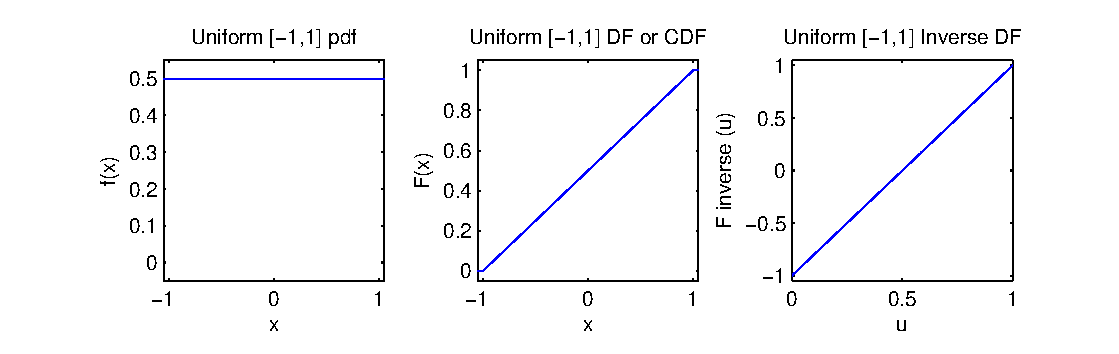
\includegraphics[width=6.5in]{figures/Unifpm1pdfcdf}}
\end{figure}

%\remove{
\begin{labwork}[Inversion Sampler Demo -- $\uniform(-5,5)$]\label{LW:guiInversionSamplerUniform}
Let us comprehend the inversion sampler by calling the interactive visual cognitive tool built by Jennifer Harlow under a grant from University of Canterbury's Centre for Teaching and Learning (UCTL):
\begin{VrbM}
>> guiInversionSampler
\end{VrbM}
The M-file {\tt guiInversionSampler.m} will bring a graphical user interface (GUI) as shown in \hyperref[F:guiInversionSamplerUniform]{Figure \ref*{F:guiInversionSamplerUniform}}.  The default target distribution is $\uniform(-5,5)$.  Now repeatedly push the ``Draw one sample'' button several times and comprehend the simulation process.  You can press ``Draw 100 samples'' to really comprehend the inversion sampler in action after 100 samples are drawn and depicted in the density histogram of the accumulating samples.  
Next try changing the numbers in the ``Lower bound'' and ``Upper bound'' boxes in order to alter the parameters $\theta_1$ and $\theta_2$ of $\uniform(\theta_1,\theta_2)$ RV.  
\end{labwork}

\begin{figure}[htpb]
\caption{Visual Cognitive Tool GUI: Inversion Sampling from $X \sim \uniform(-5,5)$.\label{F:guiInversionSamplerUniform}}
\centering   \makebox{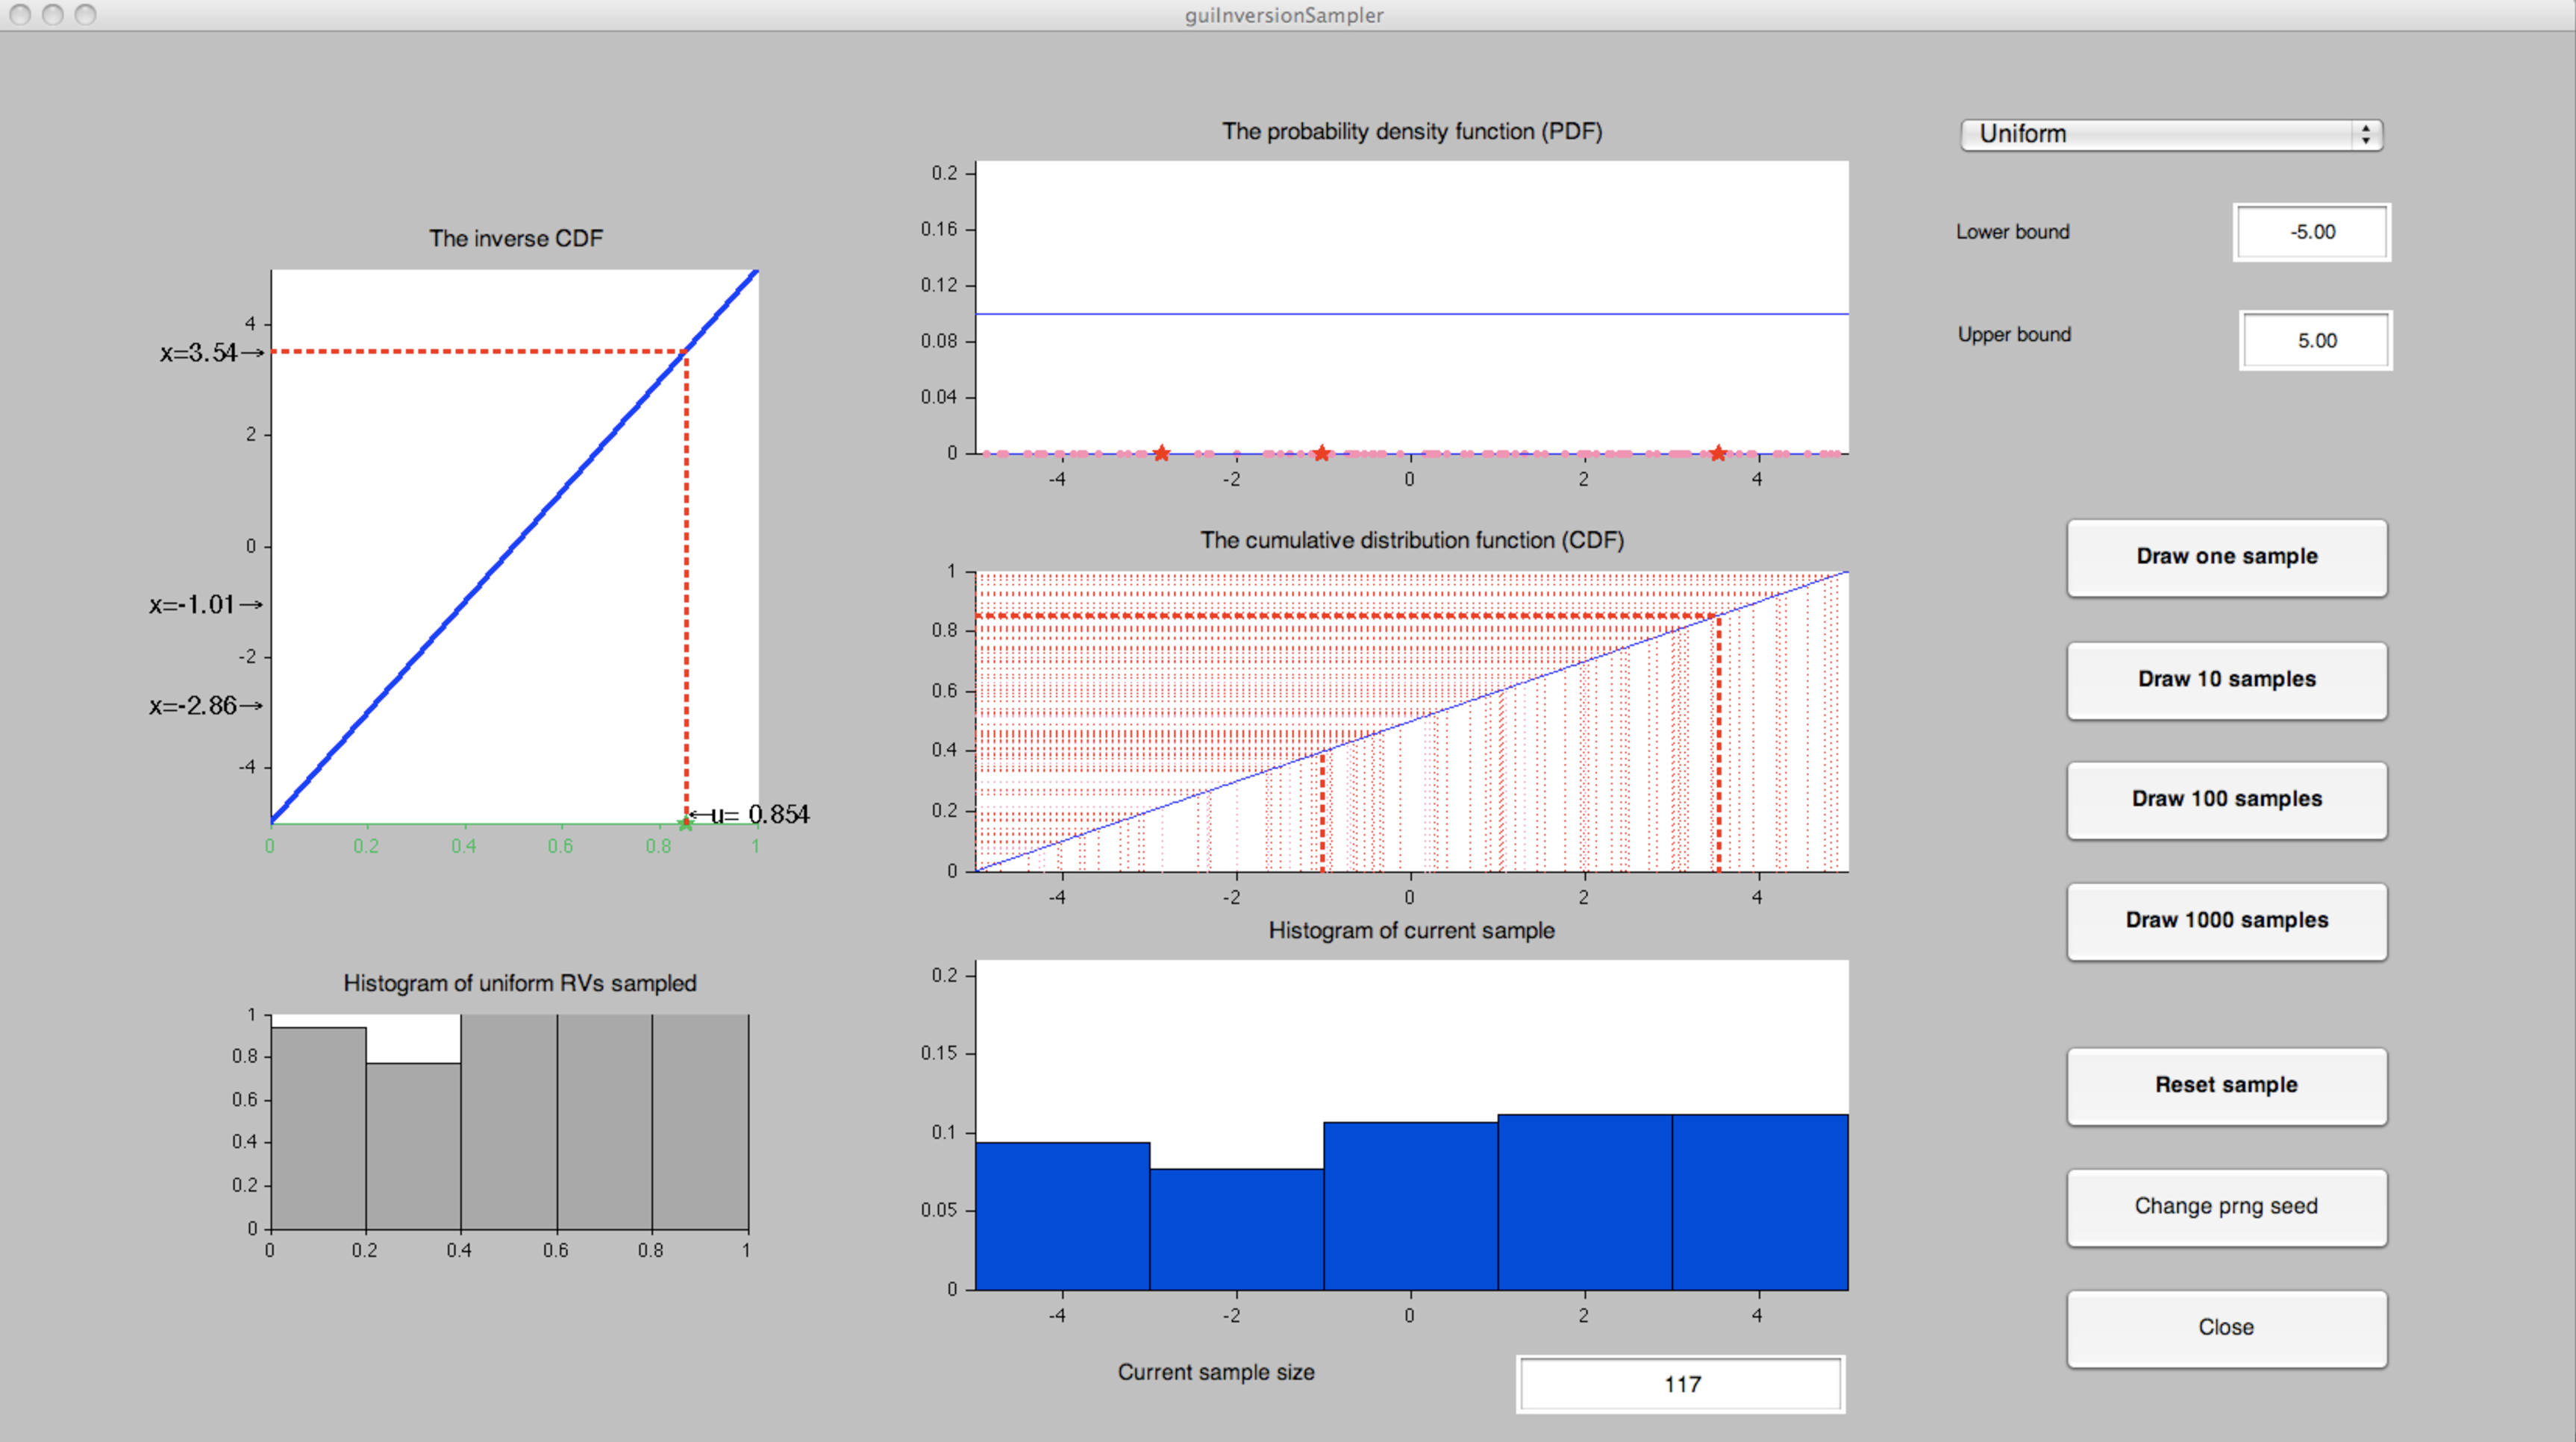
\includegraphics[width=6.50in]{figures/guiInversionSamplerUniform}}
\end{figure}

\begin{simulation}[$\uniform(\theta_1,\theta_2)$]\label{SIM:Uniformab}
To simulate from $\uniform(\theta_1,\theta_2)$ RV $X$ using the Inversion Sampler, we first need to find $F^{[-1]}(u)$ by solving for $x$ in terms of $u=F(x;\theta_1,\theta_2)$:
\[
u = \frac{x-\theta_1}{\theta_2-\theta_1} \quad \iff  \quad x = (\theta_2-\theta_1)u+\theta_1 \quad  \iff \quad  F^{[-1]}(u;\theta_1,\theta_2) = \theta_1+(\theta_2-\theta_1)u
\]
Here is a simple implementation of the Inversion Sampler for the $\uniform(\theta_1,\theta_2)$ RV in \Matlab:
\begin{VrbM}
>> rand('twister',786); % initialise the fundamental sampler for Uniform(0,1)
>> theta1=-1; theta2=1; % declare values for parameters theta1 and theta2
>> u=rand; % rand is the Fundamental Sampler and u is a sample from it
>> x=theta1+(theta2 - theta1)*u; % sample from Uniform(-1,1]) RV
>> disp(x); % display the sample from Uniform[-1,,1] RV
    0.5134
\end{VrbM}
It is just as easy to draw $n$ IID samples from $\uniform(\theta_1,\theta_2)$ RV $X$ by transforming $n$ IID samples from the $\uniform(0,1)$ RV as follows:
\begin{VrbM}
>> rand('twister',786543); % initialise the fundamental sampler
>> theta1=-83; theta2=1004; % declare values for parameters a and b
>> u=rand(1,5); % now u is an array of 5 samples from Uniform(0,1)
>> x=theta1+(theta2 - theta1)*u; % x is an array of 5 samples from Uniform(-83,1004]) RV
>> disp(x); % display the 5 samples just drawn from Uniform(-83,1004) RV
  465.3065  111.4994   14.3535  724.8881  254.0168
\end{VrbM}
%Next, we write a \Matlab function for this sampler which would take the appropriate inputs and return $n$ IID samples from a specified $Uniform(\theta_1,\theta_2)$ RV $X$.
%\VrbMf[label=UniformabSam.m]{UniformabSam.m}
\end{simulation}

%}%end remove

\begin{model}[$\exponential(\lambda)$]
For a given $\lambda > 0$, an $\exponential(\lambda)$ RV has the following PDF $f$ and DF $F$:
\begin{eqnarray}\label{E:Exponentialpdfcdf}
f(x; \lambda) = \lambda e^{-\lambda x} \qquad &
F(x; \lambda)= 1-e^{-\lambda x}  \ .
\end{eqnarray}
This distribution is fundamental because of its property of {\bf memorylessness} and plays a fundamental role in continuous time
%Markov
processes as we will see later.
\end{model}

%\remove{
We encode the PDF and DF of the $\exponential(\lambda)$ RV as \Matlab functions {\tt ExponentialPdf} and {\tt ExponentialCdf} and use them to produce \hyperref[F:plotPdfCdfExponentials]{Figure~\ref*{F:plotPdfCdfExponentials}} in \hyperref[Mf:ExponentialPdfCdf]{Labwork~\ref*{Mf:ExponentialPdfCdf}}.
%}%end remove

\begin{figure}[htpb]
\caption{Density and distribution functions of $Exponential(\lambda)$ RVs, for $\lambda=1, 10, 10^{-1}$, in four different axes scales.\label{F:plotPdfCdfExponentials}}
\centering   \makebox{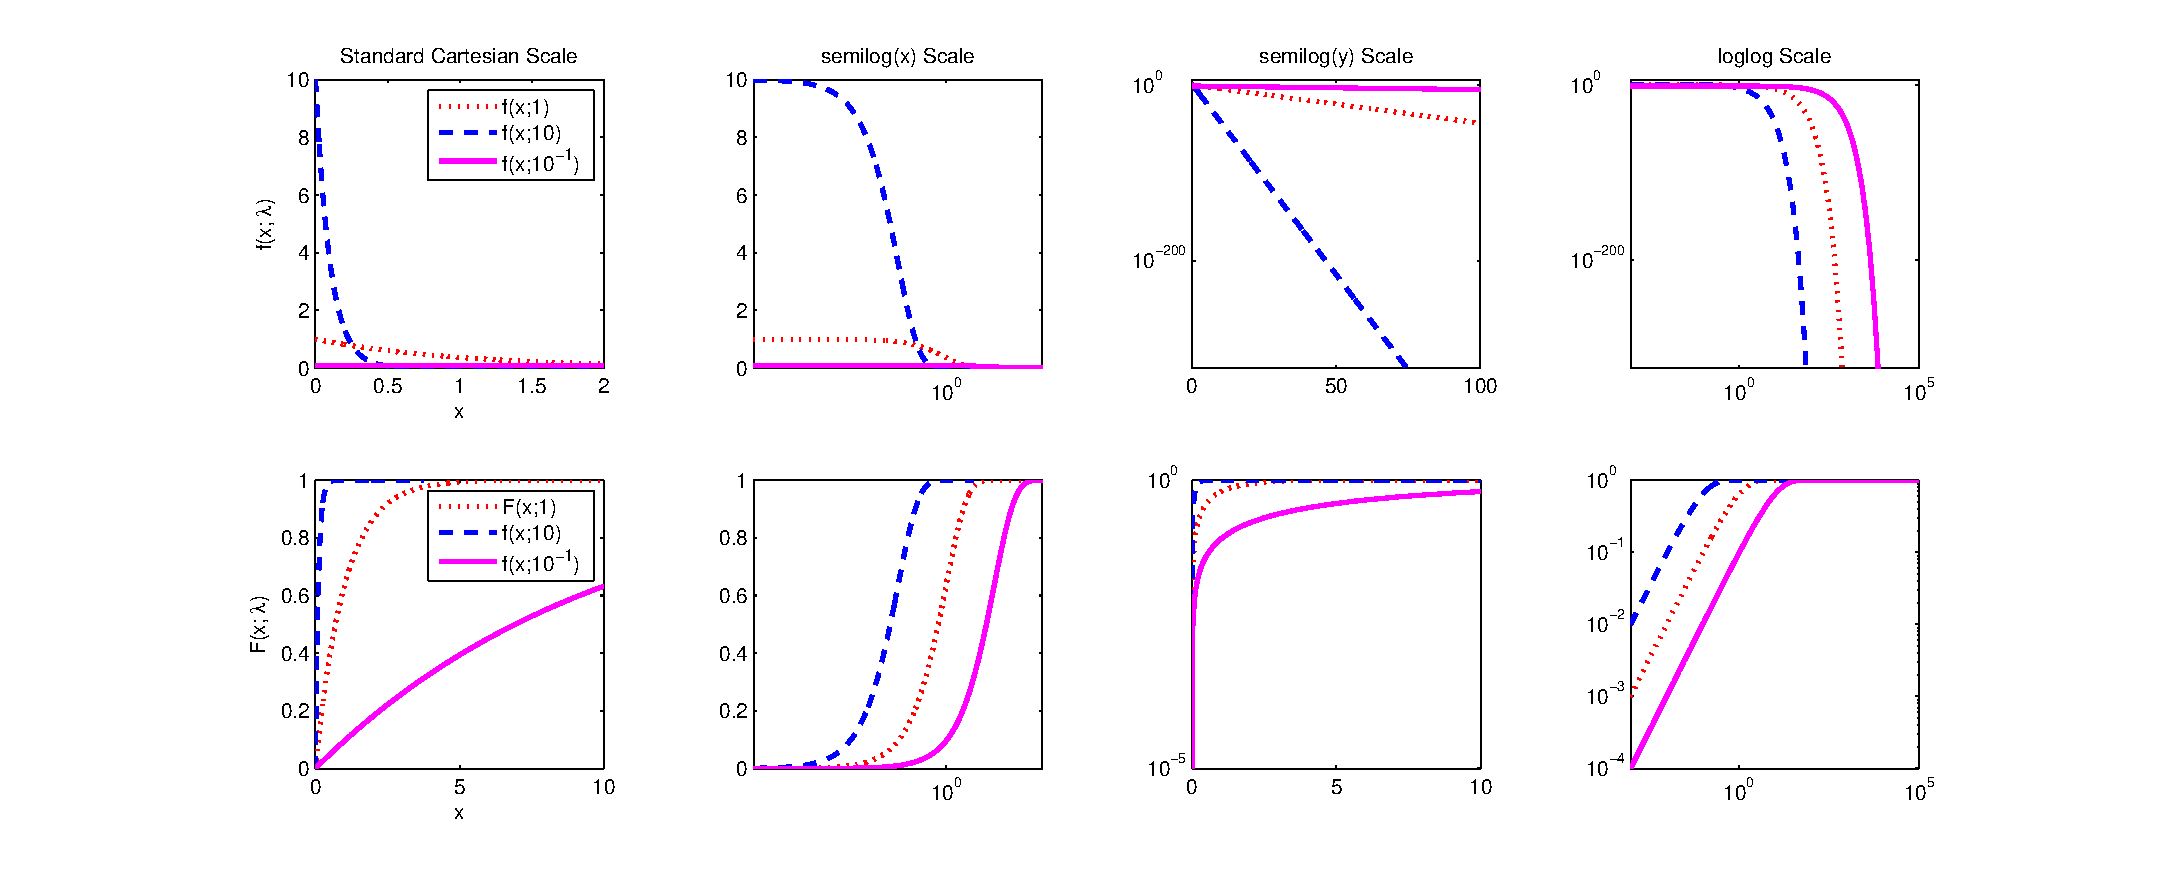
\includegraphics[width=6.5in]{figures/plotPdfCdfExponentials}}
\end{figure}

\paragraph{Mean and Variance of $\exponential(\lambda)$:}
Show that the mean of an $\exponential(\lambda)$ RV $X$ is:
\[
\e_{\lambda}(X) = \int_{0}^{\infty} x f(x;\lambda)\,dx
=   \int_{0}^{\infty} x \lambda e^{-\lambda x}\,dx
= \frac{1}{\lambda} \ ,
\]
and the variance is:
\[
\V_{\lambda}(X) = \left(  \frac{1}{\lambda} \right)^2 \ .
\]

%\remove{
\begin{labwork}[Inversion Sampler Demo -- $\exponential(0.5)$]\label{LW:guiInversionSamplerExponential}
Let us understand the inversion sampler by calling the interactive visual cognitive tool:
\begin{VrbM}
>> guiInversionSampler
\end{VrbM}
The M-file {\tt guiInversionSampler.m} will bring a graphical user interface (GUI) as shown in \hyperref[F:guiInversionSamplerExponential]{Figure \ref*{F:guiInversionSamplerExponential}}.  First change the target distribution from the default $\uniform(-5,5)$ to $\exponential(0.5)$ from the drop-down menu.  Now push the ``Draw 10 samples'' button and comprehend the simulation process.  Next try changing the ``Rate Parameter'' from $0.5$ to $10.0$ for example  and generate several inversion samples and see the density histogram of the accumulating samples.  You can press ``Draw one sample'' to really comprehend the inversion sampler in action one step at a time.
\end{labwork}

\begin{figure}[htpb]
\caption{Visual Cognitive Tool GUI: Inversion Sampling from $X \sim \exponential(0.5)$.\label{F:guiInversionSamplerExponential}}
\centering   \makebox{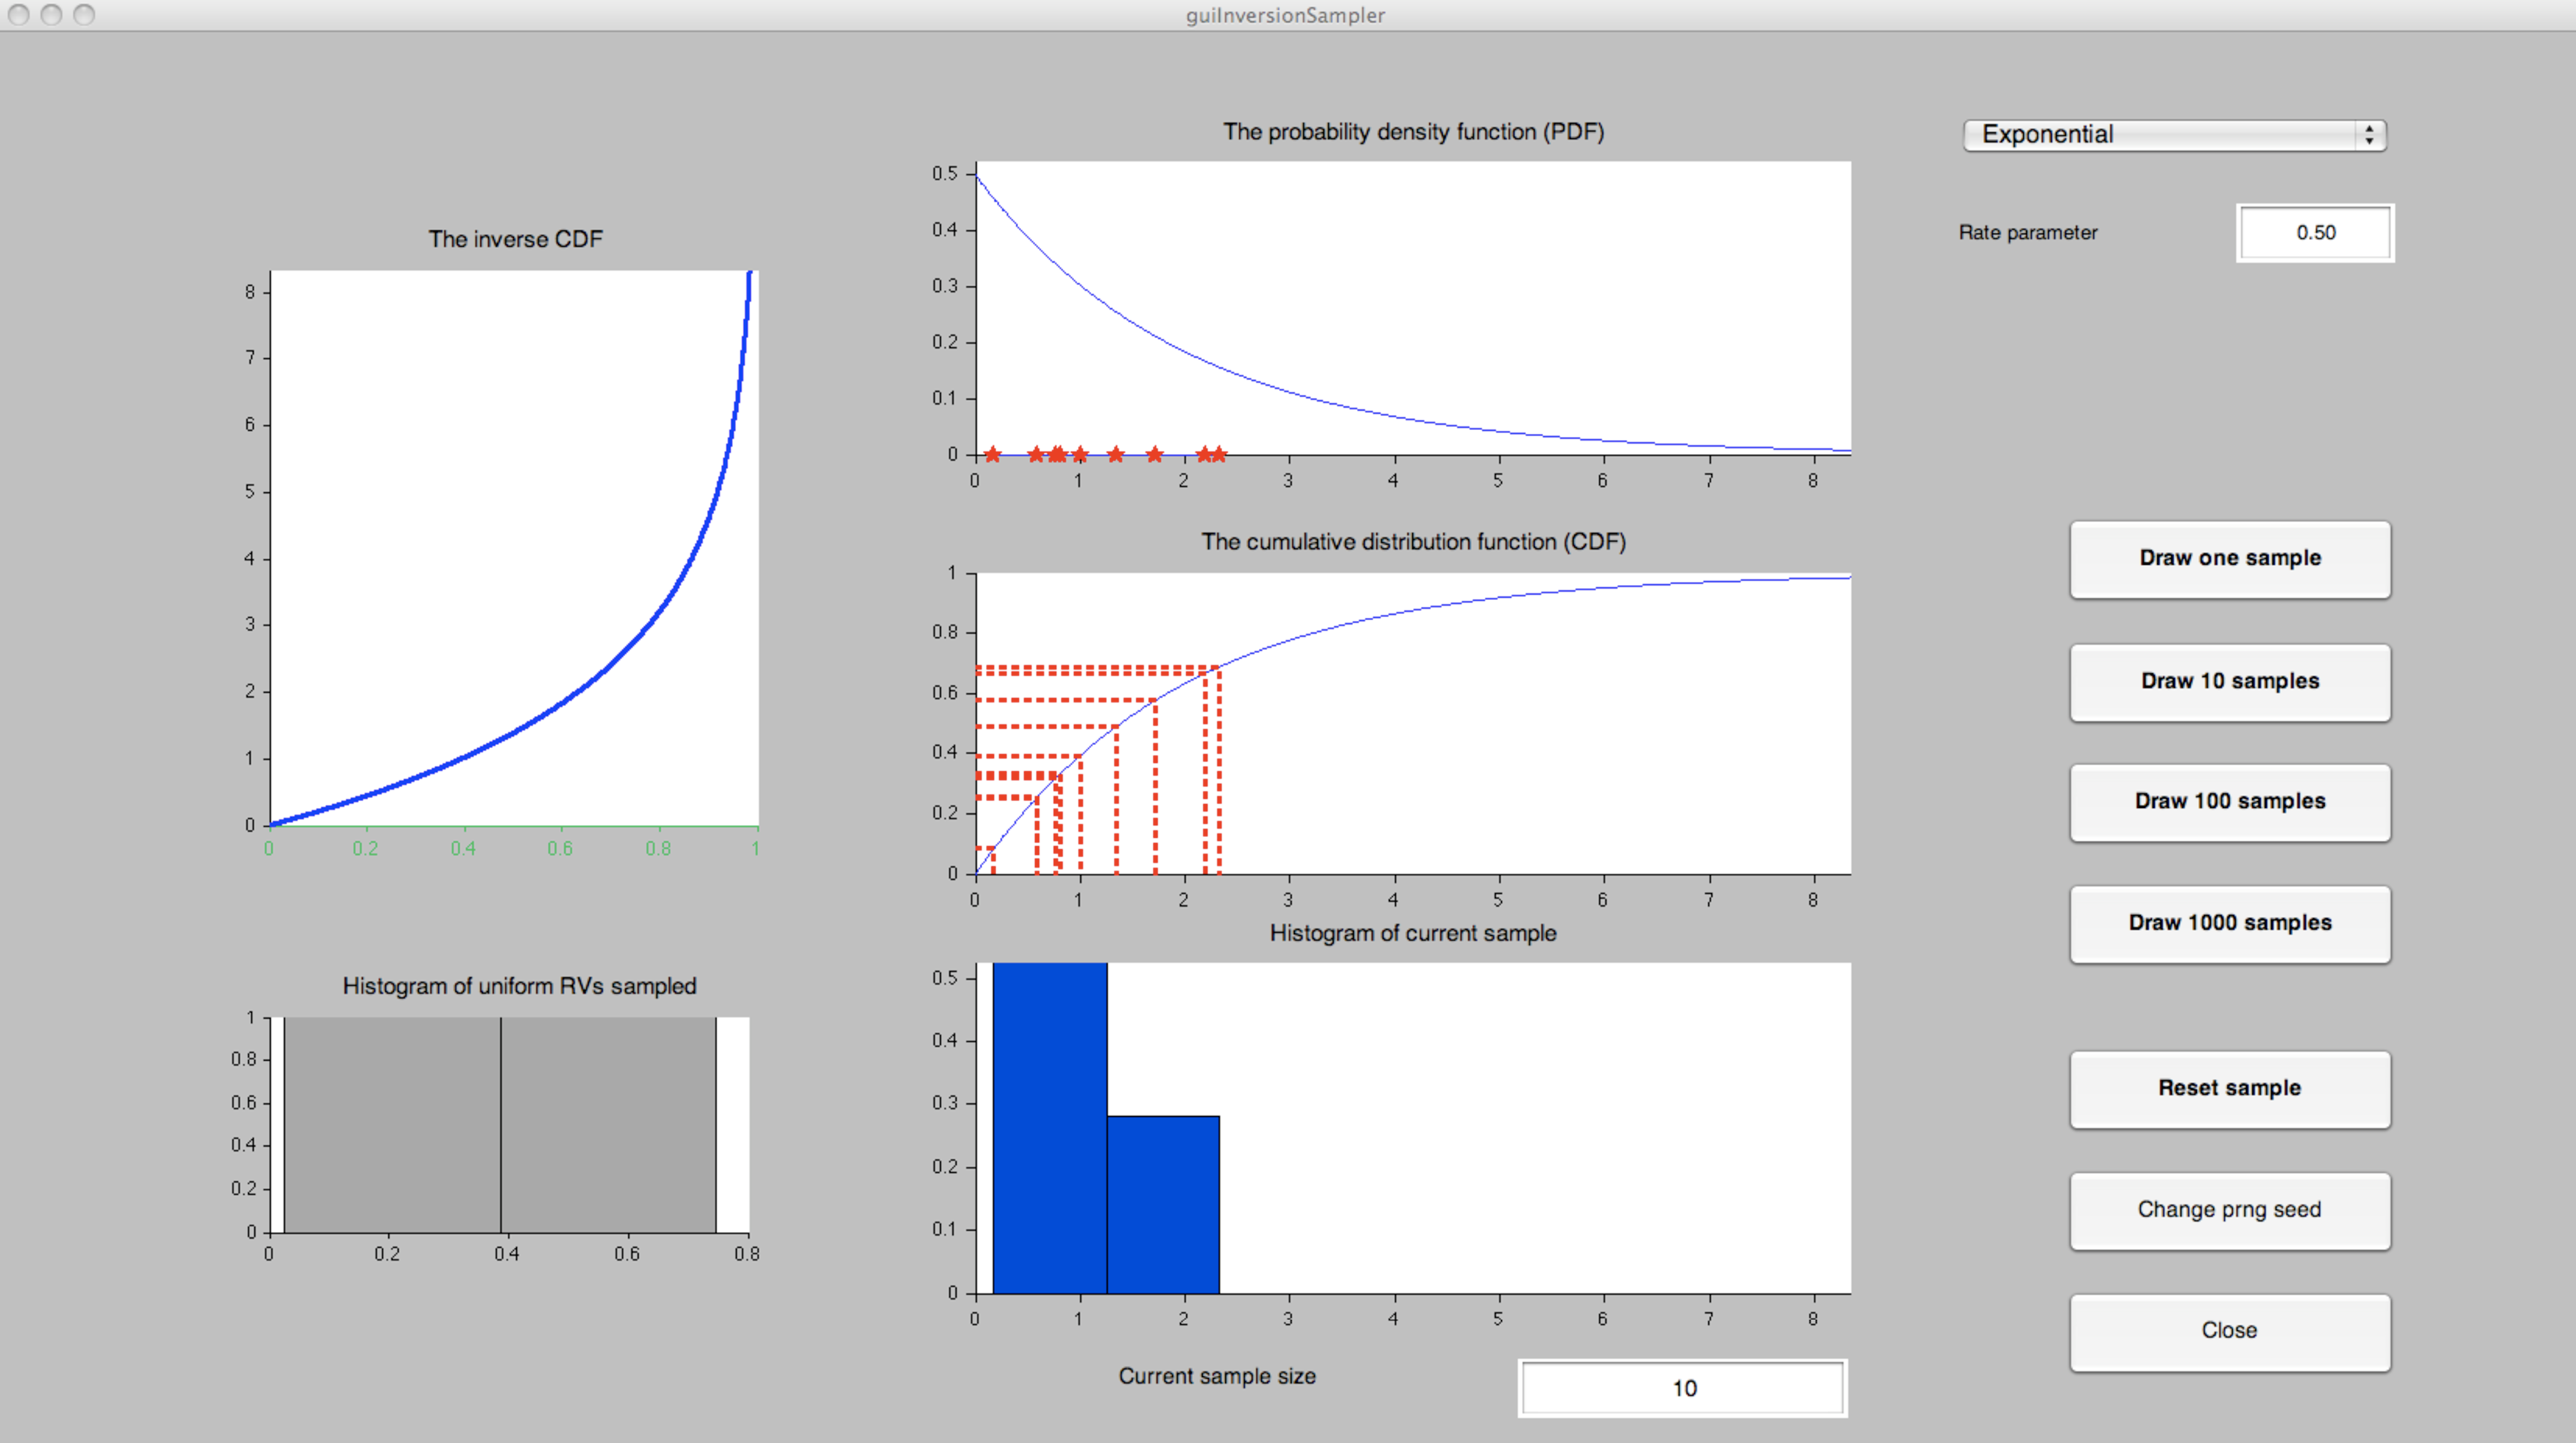
\includegraphics[width=6.50in]{figures/guiInversionSamplerExponential}}
\end{figure}

Let us consider the problem of simulating from an $\exponential(\lambda)$ RV with realisations in $\Rz_+ := [0,\infty) := \{x: x \geq 0, x \in \Rz\}$ to model the waiting time for a bus at a bus stop.
\begin{simulation}[$\exponential(\lambda)$]\label{SIM:Exponential}
For a given $\lambda > 0$, an $\exponential(\lambda)$ RV has the following PDF $f$, DF $F$ and inverse DF $F^{[-1]}$:
\begin{eqnarray}
f(x; \lambda) = \lambda e^{-\lambda x} \quad &
F(x; \lambda)= 1-e^{-\lambda x} \quad &
F^{[-1]}(u; \lambda)= \frac{-1}{\lambda} \log_e (1-u)
\end{eqnarray}
We write the natural logarithm $\log_e$ as $\log$ for notational simplicity.  An implementation of the Inversion Sampler for $\exponential(\lambda)$ as a function in the M-file:
\VrbMf[label=ExpInvCDF.m]{scripts/ExpInvCDF.m}
We can simply call the function to draw a sample from, say the $\exponential(\lambda=1.0)$ RV by:
\begin{VrbM}
  lambda=1.0;			% some value for lambda
  u=rand;			% rand is the Fundamental Sampler
  ExpInvCDF(u,lambda)	% sample from Exponential(1) RV via function in ExpInvCDF.m
\end{VrbM}
Because of the following:
\[
 U \sim \uniform(0,1) \quad \implies \quad
 -U \sim \uniform(-1,0) \quad \implies \quad
 1-U \sim \uniform(0,1)  \  ,
 \]
 we could save a subtraction operation in the above algorithm by replacing {\tt -(1/lambda) * log(1-u)} by {\tt -(1/lambda) * log(u)}.  This is implemented as the following function.
 \VrbMf[label=ExpInvSam.m]{scripts/ExpInvSam.m}
\begin{VrbM}
>> rand('twister',46678); % initialise the fundamental sampler
>> Lambda=1.0;  % declare Lambda=1.0
>> x=ExpInvSam(rand(1,5),Lambda); % pass an array of 5 Uniform(0,1) samles from rand
>> disp(x); % display the Exponential(1.0) distributed samples
    0.5945    2.5956    0.9441    1.9015    1.3973
\end{VrbM}
 % Get a concrete understanding by implementing this simulation in Lab.
\end{simulation}

\begin{figure}[htpb]
\caption{The PDF $f$, DF $F$, and inverse DF $F^{[-1]}$ of the the $\exponential(\lambda=1.0)$ RV. \label{F:ExpfFFInv}}
\centering   \makebox{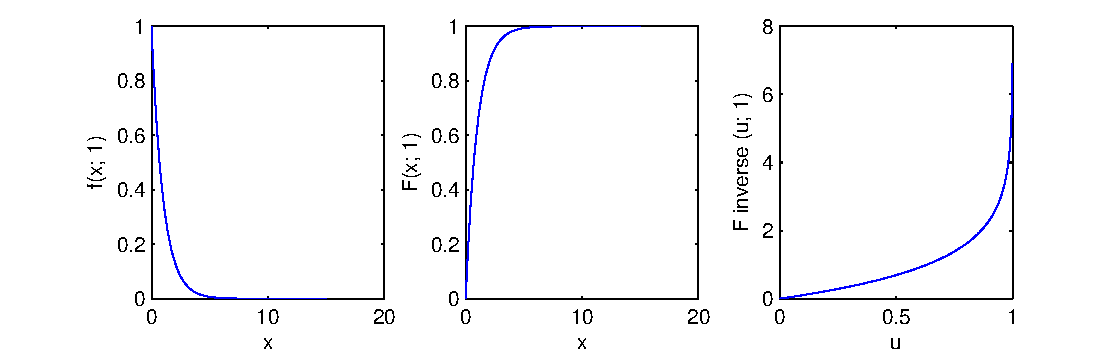
\includegraphics[width=6.5in]{figures/plotExpfFFInv}}
\end{figure}

It is straightforward to do replicate experiments.  Consider the experiment of drawing five  independent samples from the $\exponential(\lambda=1.0)$ RV.  Suppose we want to repeat or replicate this experiment seven times and find the sum of the five outcomes in each of these replicates.  Then we may do the following:

\begin{VrbM}
>> rand('twister',1973); % initialise the fundamental sampler
>> % store 7 replications of 5 IID draws from Exponential(1.0) RV in array a
>> lambda=1.0; a= -1/lambda * log(rand(5,7)); disp(a);
    0.7267    0.3226    1.2649    0.4786    0.3774    0.0394    1.8210
    1.2698    0.4401    1.6745    1.4571    0.1786    0.4738    3.3690
    0.4204    0.1219    2.2182    3.6692    0.9654    0.0093    1.7126
    2.1427    0.1281    0.8500    1.4065    0.1160    0.1324    0.2635
    0.6620    1.1729    0.6301    0.6375    0.3793    0.6525    0.8330
>> %sum up the outcomes of the sequence of 5 draws in each replicate
>> s=sum(a); disp(s);
    5.2216    2.1856    6.6378    7.6490    2.0168    1.3073    7.9990
\end{VrbM}

\begin{labwork}[Next seven buses at your bus-stop]\label{LW:Next7Buses}
Consider the problem of modelling the arrival of buses at a bus stop.  Suppose that the time between arrivals is an $\exponential(\lambda=0.1)$ RV $X$ with a mean inter-arrival time of $1/\lambda=10$ minutes.  Suppose you go to your bus stop and zero a stop-watch.  Simulate the times of arrival for the next seven buses as indicated by your stop-watch.  Seed the fundamental sampler by your Student ID (eg.~if your ID is {\tt 11424620} then type {\tt rand('twister', 11424620);} just before the simulation).  Hand in the code with the arrival times of the next seven buses at your ID-seeded bus stop.
\end{labwork}

The support of the $\exponential(\lambda)$ RV is $\Rz_+ := [0,\infty)$.  Let us consider a RV built by mirroring the $\exponential(\lambda)$ RV about the origin with the entire real line as its support.
\begin{model}[$\laplace(\lambda)$ or $\doubleexponential(\lambda)$ RV]
If a RV $X$ is equally likely to be either positive or negative with an exponential density, then the $\laplace(\lambda)$ or $\doubleexponential(\lambda)$ RV, with the rate parameter $\lambda>0, \lambda \in \Rz$, may be used to model it.  The density function for the $\laplace(\lambda)$ RV given by $f(x; \lambda)$ is
\begin{equation}\label{E:Laplacepdf}
f(x; \lambda) = \frac{\lambda}{2} e^{- \lambda |x|} =
\begin{cases}
 \frac{\lambda}{2} e^{ \lambda x} & \text{if $x < 0$} \\
 \frac{\lambda}{2} e^{- \lambda x} & \text{if $x \geq 0$} \\
\end{cases}
\enspace .
\end{equation}
Let us define the sign of a real number $x$ by
\[
\sign(x) =
\begin{cases}
~~1 & \text{if $x > 0$} \\
~~0 & \text{if $x = 0$} \\
-1 & \text{if $x < 0$}  \ . \\
\end{cases}
\]
Then, the DF of the $\laplace(\lambda)$ RV $X$ is
\begin{equation} \label{E:Laplacecdf}
F(x; \lambda) = \int_{-\infty}^{x} f(y; \lambda)\,dy = \frac{1}{2}\left(1+ \sign(x) \left(1-e^{- \lambda |x|}\right) \right) \ ,
\end{equation}
and its inverse DF is
\begin{equation}\label{E:LaplaceInvcdf}
F^{[-1]}(u;\lambda) = - \frac{1}{\lambda} \ \sign\left(u-\frac{1}{2}\right) \log \left(1 - 2 \left|u-\frac{1}{2} \right| \right) \ , \ u \in [0,1]
\end{equation}
\end{model}

\paragraph{Mean and Variance of $\laplace(\lambda)$ RV $X$:}
Show that the mean of a $\laplace(\lambda)$ RV $X$ is
\[
\e(X) = \int_{0}^{\infty} x f(x;\lambda)\,dx
=   \int_{0}^{\infty} x \frac{\lambda}{2} e^{- \lambda |x|}\,dx
= 0 \ ,
\]
and the variance is
\[
\V(X) = \left(  \frac{1}{\lambda} \right)^2 + \left(  \frac{1}{\lambda} \right)^2 = 2 \left(  \frac{1}{\lambda} \right)^2\ .
\]
Note that the mean is $0$ due to the symmetry of the density about $0$ and the variance is twice that of the $\exponential(\lambda)$ RV.

\begin{labwork}[Rejection Sampler Demo -- $\laplace(5)$]\label{LW:guiInversionSamplerLaplace}
Let us comprehend the rejection sampler by calling the interactive visual cognitive tool:
\begin{VrbM}
>> guiInversionSampler
\end{VrbM}
The M-file {\tt guiInversionSampler.m} will bring a graphical user interface (GUI) as shown in \hyperref[F:guiInversionSamplerLaplace]{Figure \ref*{F:guiInversionSamplerLaplace}}.  Using the drop-down menu change from the default target distribution $\uniform(-5,5)$ to $\laplace(5)$.  Now repeatedly push the ``Draw one sample'' button several times and comprehend the simulation process.  You can also press ``Draw 1000 samples'' and see the density histogram of the generated samples.  
Next try changing the numbers in the ``Rate parameter'' box from $5.00$ to $1.00$ in order to alter the parameter $\lambda$ of $\laplace(\lambda)$ RV.  If you are more adventurous then try to alter the number in the ``Location parameter'' box from $0.00$ to some thing else, say $10.00$.  Although our formulation of $\laplace(\lambda)$ implicitly had a location parameter of $0.00$, we can easily introduce a location parameter $\mu$ into the PDF.  With a pencil and paper try to rewrite the PDF in \eqref{E:Laplacepdf} with an additional location parameter $\mu$.
\end{labwork}

\begin{figure}[htpb]
\caption{Visual Cognitive Tool GUI: Inversion Sampling from $X \sim \laplace(5)$.\label{F:guiInversionSamplerLaplace}}
\centering   \makebox{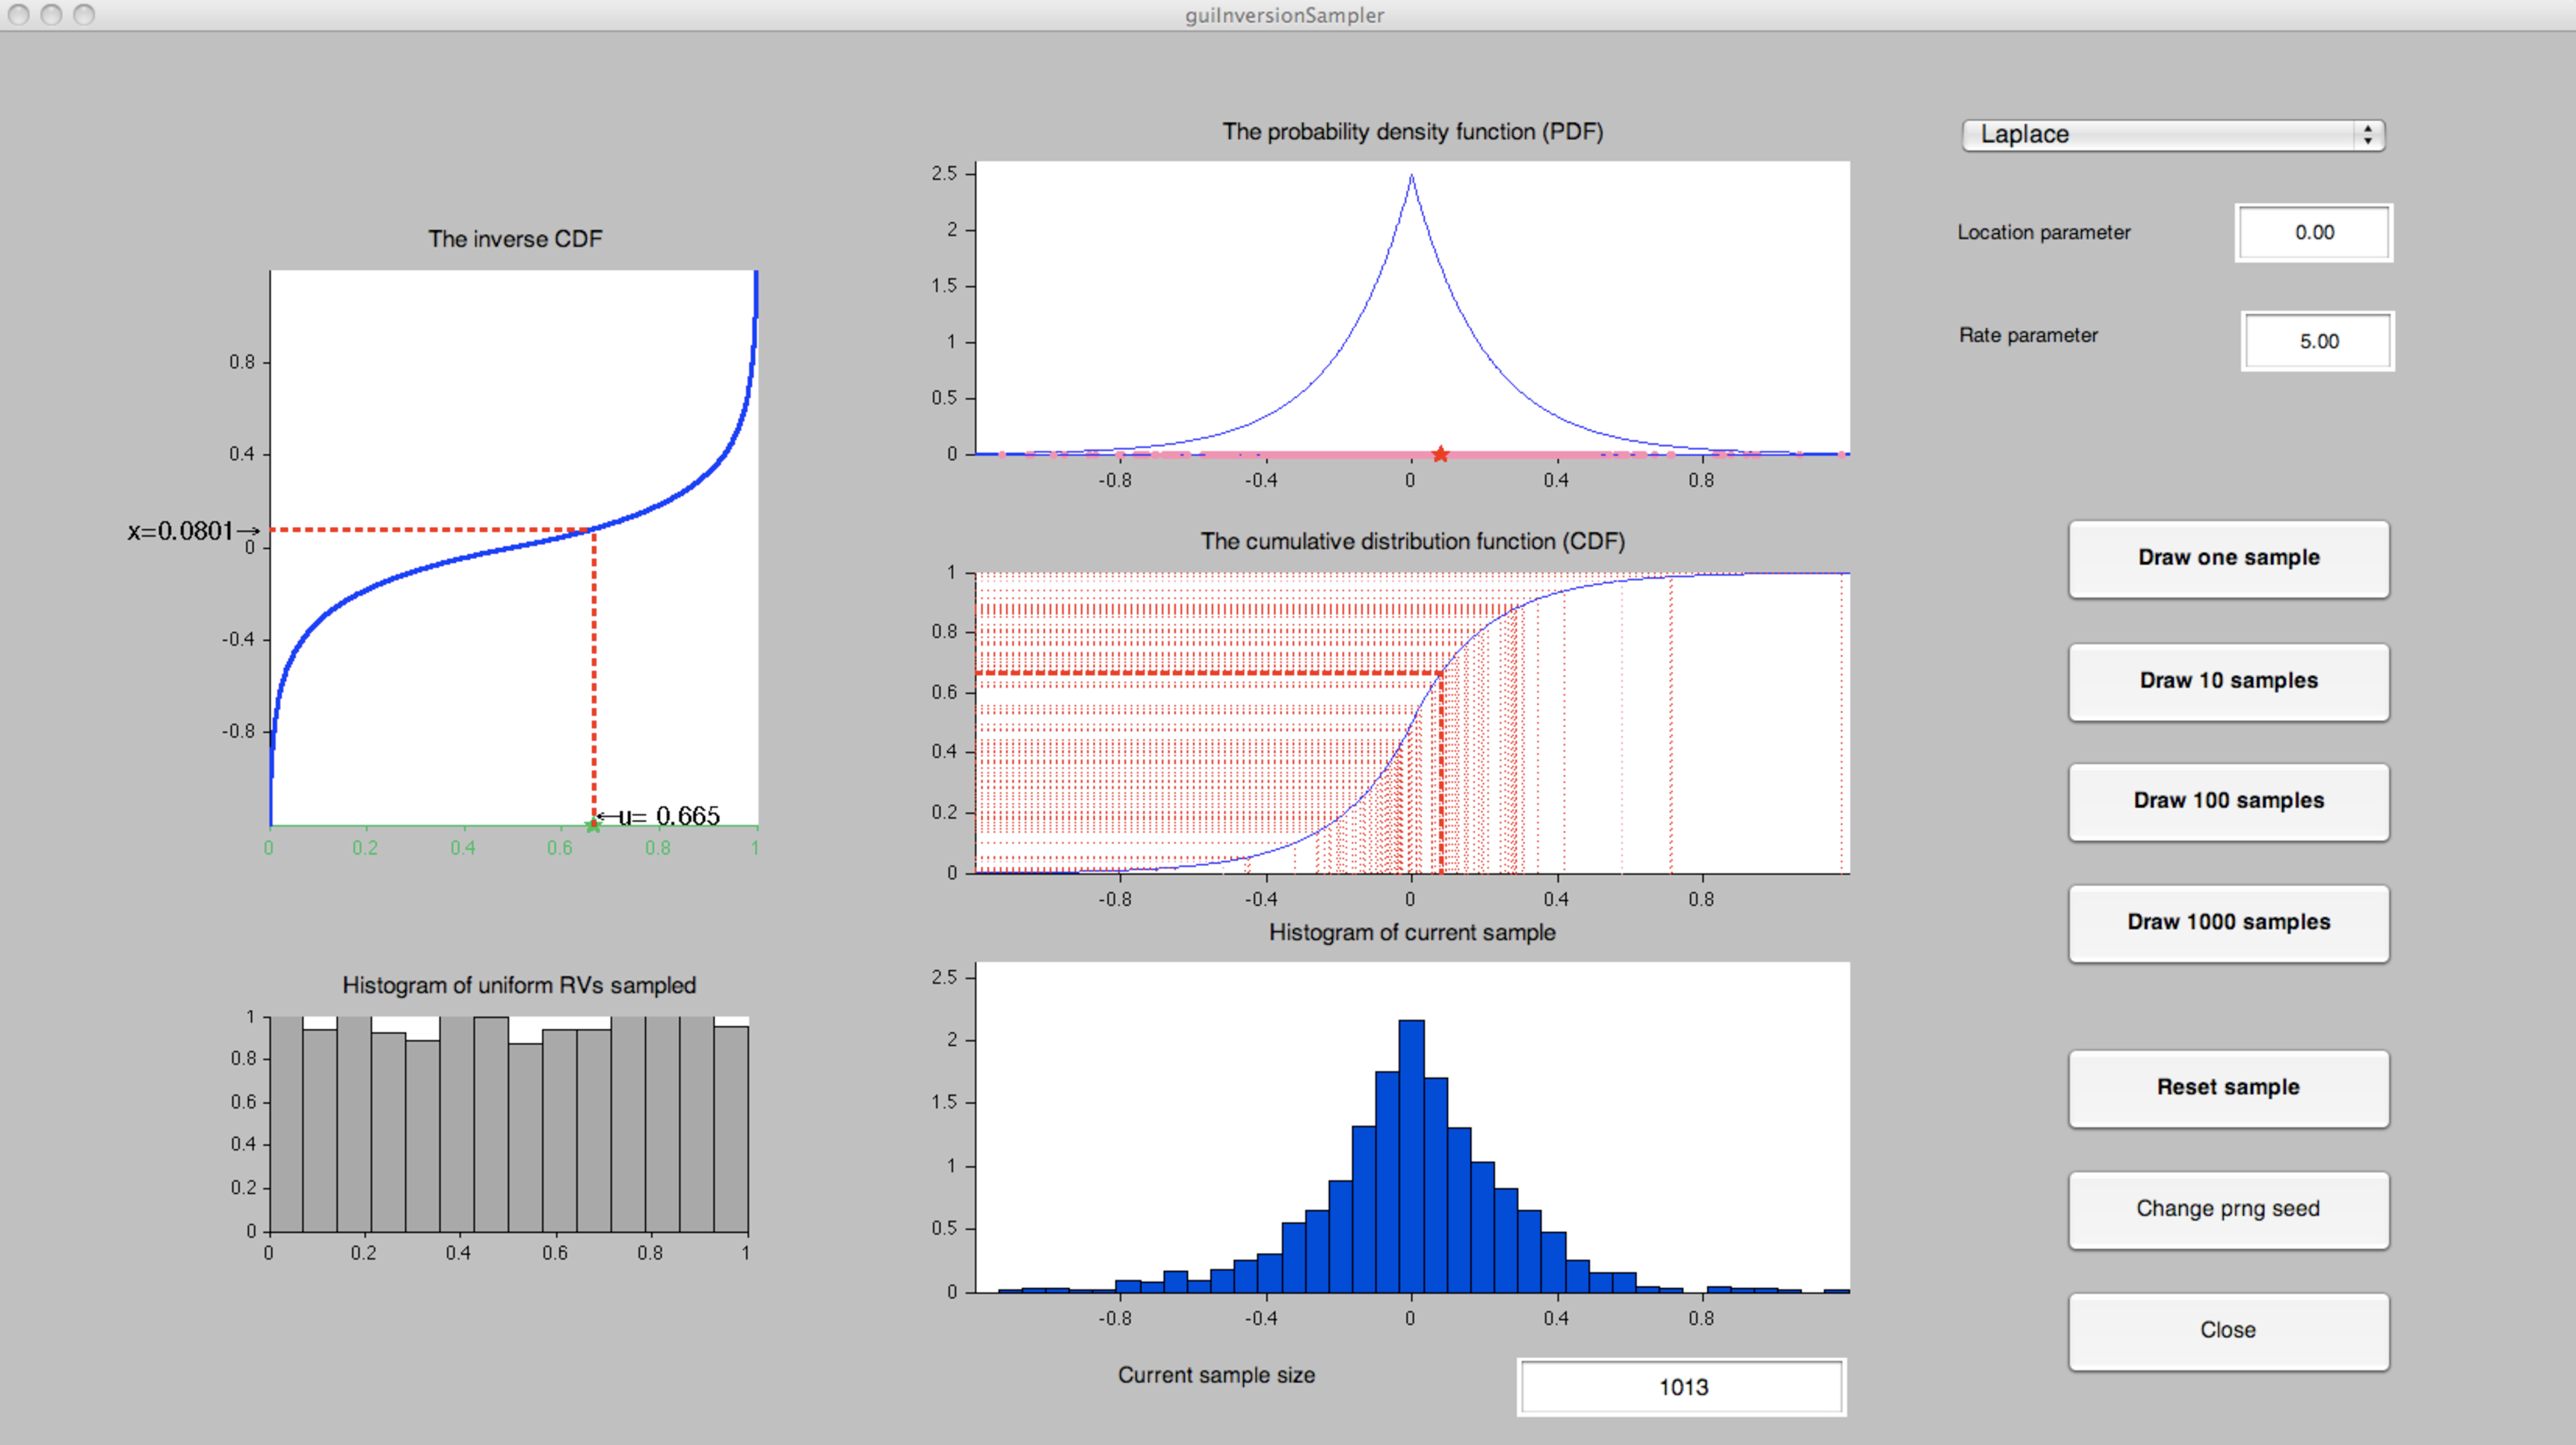
\includegraphics[width=6.50in]{figures/guiInversionSamplerLaplace}}
\end{figure}

\begin{simulation}[$\laplace(\lambda)$] \label{SIM:Laplace}
Here is an implementation of an inversion sampler to draw IID samples from a $\laplace(\lambda)$ RV $X$ by transforming IID samples from the $\uniform(0,1)$ RV $U$:
\VrbMf[label=LaplaceInvCDF.m]{scripts/LaplaceInvCDF.m}
We can simply call the function to draw a sample from, say the $\laplace(\lambda=1.0)$ RV by
\begin{VrbM}
>> lambda=1.0;		% some value for lambda
>> rand('twister',6567);        % initialize the fundamental sampler
>> u=rand(1,5);		% draw 5 IID samples from Uniform(0,1) RV
>> disp(u);		% display the samples in u
    0.6487    0.9003    0.3481    0.6524    0.8152

>> x=LaplaceInvCDF(u,lambda); % draw 5 samples from Laplace(1) RV using inverse CDF
>> disp(x);                     % display the samples
    0.3530    1.6127   -0.3621    0.3637    0.9953
\end{VrbM}
\end{simulation}

%}%end remove

Next, let us become familiar with an RV for which the expectation does not exist.  This will help us appreciate the phrase ``none of which is dominant'' in the informal statement of the CLT later.
\begin{model}[$\cauchy$]
The density of the $\cauchy$ RV $X$ is:
\begin{equation}\label{E:StandardCauchypdf}
f(x) = \frac{1}{\pi (1+x^2)}, \qquad -\infty < x < \infty \enspace ,
\end{equation}
and its DF is:
\begin{equation}\label{E:StandardCauchycdf}
F(x) = \frac{1}{\pi} \tan^{-1} (x) + \frac{1}{2} \ .
\end{equation}
Randomly spinning a LASER emitting improvisation of ``Darth Maul's double edged lightsaber'' that is centered at $(1,0)$ in the plane $\Rz^2$ and recording its intersection with the $y$-axis, in terms of the $y$ coordinates, gives rise to the $Standard~Cauchy$ RV.
\end{model}

\paragraph{Mean of $\cauchy$ RV:}
The expectation of the $\cauchy$ RV $X$, obtained via integration by parts (set $u=x$ and $v=tan^{-1}(x)$) does not exist  %\eqref{E:ExpectationExists}
, since:
\begin{equation}\label{E:CauchyMeanDoesNotExist}
\int \left|x\right|\,dF(x) = \frac{2}{\pi} \int_0^{\infty} \frac{x}{1+x^2}\,dx = \left(x \tan^{-1}(x) \right]_0^{\infty} - \int_0^{\infty} \tan^{-1}(x)\, dx = \infty \ .
\end{equation}
Variance and higher moments cannot be defined when the expectation itself is undefined.

%\remove{
\begin{labwork}[Inversion Sampler Demo -- $\cauchy$]\label{LW:guiInversionSamplerCauchy}
Let us comprehend the inversion sampler by calling the interactive visual cognitive tool:
\begin{VrbM}
>> guiInversionSampler
\end{VrbM}
The M-file {\tt guiInversionSampler.m} will bring a graphical user interface (GUI) as shown in \hyperref[F:guiInversionSamplerCauchy]{Figure \ref*{F:guiInversionSamplerCauchy}}.  Using the drop-down menu change from the default target distribution $\uniform(-5,5)$ to $\cauchy$.  Now repeatedly push the ``Draw one sample'' button several times and comprehend the simulation process.  You can also press ``Draw 10 samples'' several times and see the density histogram of the generated samples.  
Next try changing the numbers in the ``Scale parameter'' and ``Location Parameter'' boxes from the default values of $1.00$ and  $0.00$, respectively.  Although our formulation of $\cauchy$ RV is also called {\em Standard Cauchy} as it implicitly had a location parameter of $0.00$ and scale parameter of $1$.  With a pencil and paper (in conjunction with a wikipedia search if you have to) try to rewrite the PDF in \eqref{E:StandardCauchypdf} with an additional location parameter $\mu$ and scale parameter $\sigma$.
\end{labwork}

\begin{figure}[htpb]
\caption{Visual Cognitive Tool GUI: Inversion Sampling from $X \sim \cauchy$.\label{F:guiInversionSamplerCauchy}}
\centering   \makebox{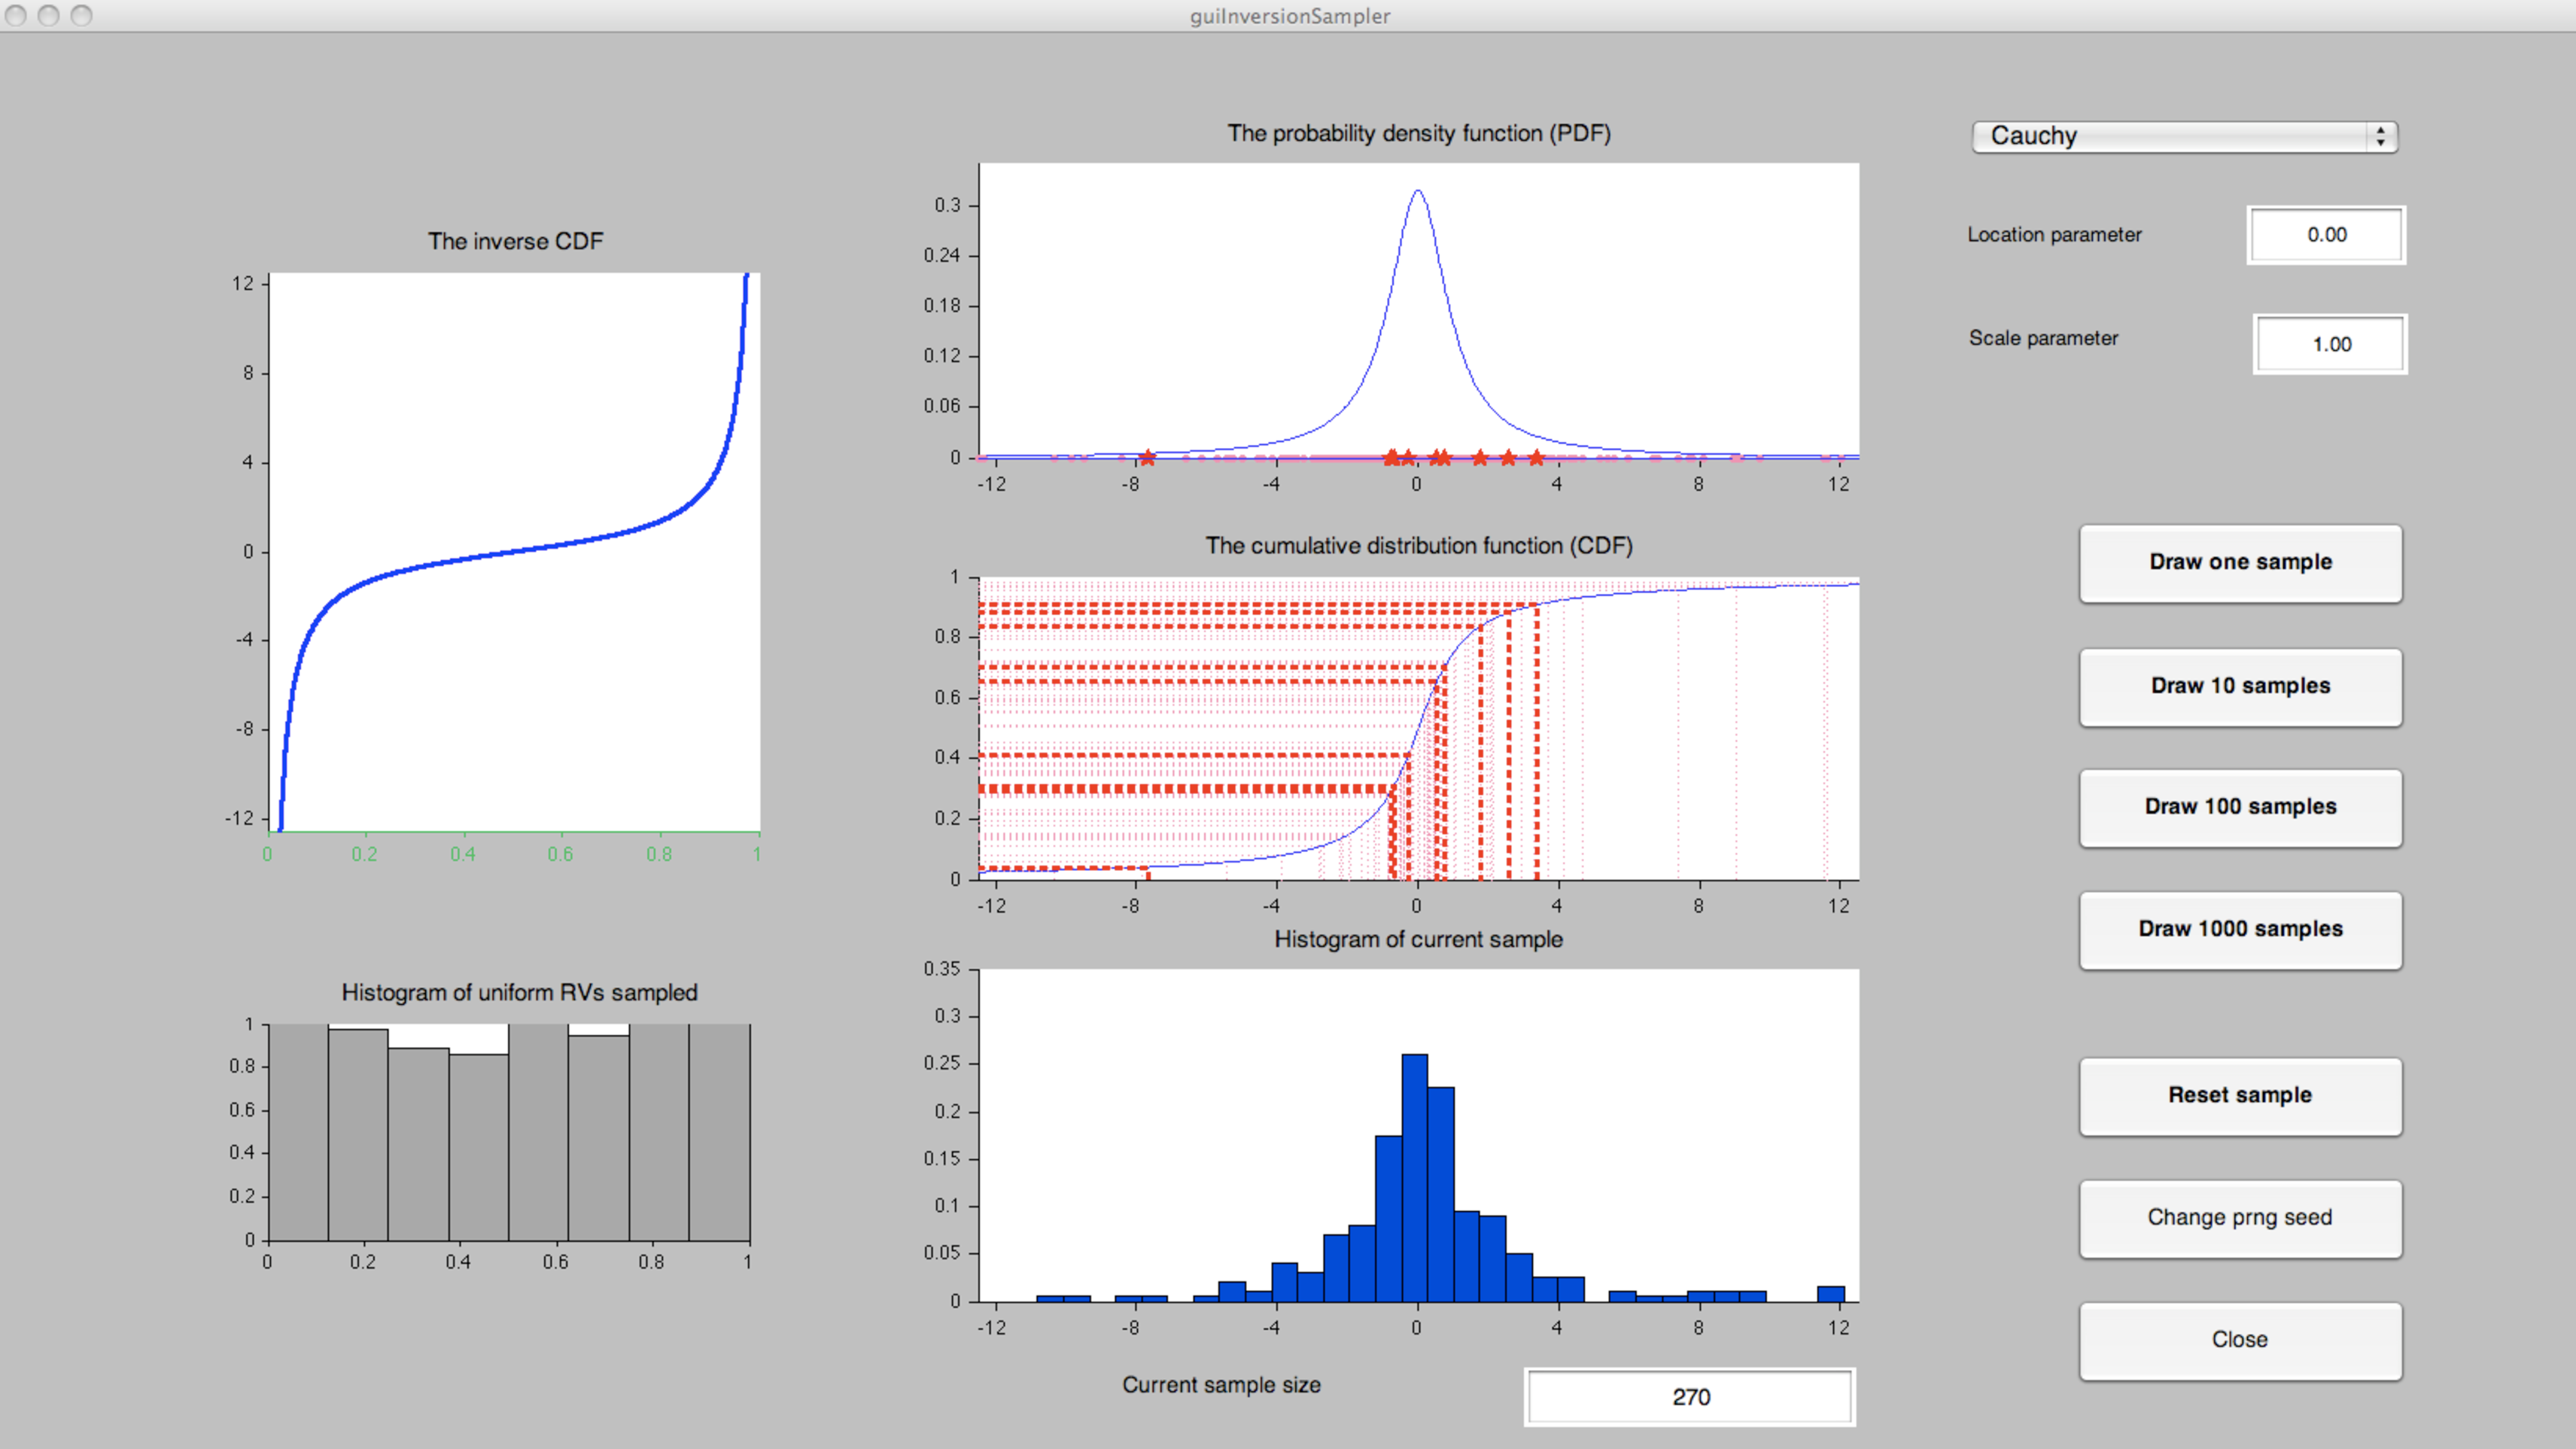
\includegraphics[width=6.50in]{figures/guiInversionSamplerCauchy}}
\end{figure}

\begin{simulation}[$\cauchy$]\label{SIM:StdCauchy}
We can draw $n$ IID samples from the $\cauchy$ RV $X$ by transforming $n$ IID samples from $\uniform(0,1)$ RV $U$ using the inverse DF as follows:
\begin{VrbM}
>> rand('twister',2435567);        % initialise the fundamental sampler
>> u=rand(1,5);			% draw 5 IID samples from Uniform(0,1) RV
>> disp(u);			% display the samples in u
    0.7176    0.6655    0.9405    0.9198    0.2598
>> x=tan(pi * u);     % draw 5 samples from Standard cauchy RV using inverse CDF
>> disp(x);  % display the samples in x
   -1.2272   -1.7470   -0.1892   -0.2575    1.0634
\end{VrbM}
\end{simulation}
 Recall that the mean of the $\cauchy$ RV $X$ does not exist since $\int \left|x\right|\,dF(x) = \infty$ \eqref{E:CauchyMeanDoesNotExist}.  We will investigate this in \hyperref[LW:RunningMeanCauchy]{Labwork~\ref*{LW:RunningMeanCauchy}}.

 \begin{labwork}[Running mean of the Standard Cauchy RV]\label{LW:RunningMeanCauchy}
Let us see what happens when we plot the running sample mean for an increasing sequence of IID samples from the Standard Cauchy RV $X$ by implementing the following script file:
 \VrbMf[label=PlotStandardCauchyRunningMean.m]{scripts/PlotStandardCauchyRunningMean.m}

%}%end remove

\begin{figure}[htpb]
\caption{Unending fluctuations of  the running means based on $n$ IID samples from the Standard $\cauchy$ RV $X$ in each of five replicate simulations (blue lines).  The running means, based on $n$ IID samples from the $\uniform(0,10)$ RV, for each of five replicate simulations (magenta lines). \label{F:plot5RunningMeansStandardcauchyUnif010}}
\centering   \makebox{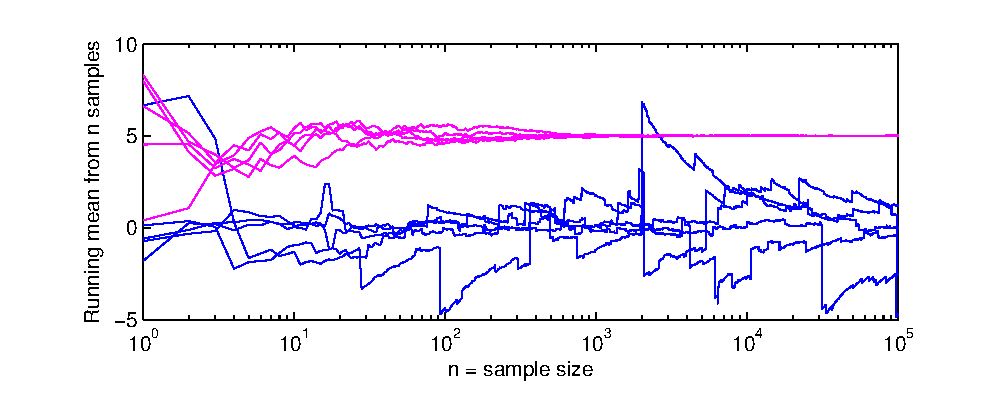
\includegraphics[width=5.5in]{figures/plot5RunningMeansStandardcauchyUnif010}}
\end{figure}

The resulting plot is shown in \hyperref[F:plot5RunningMeansStandardcauchyUnif010]{Figure~\ref*{F:plot5RunningMeansStandardcauchyUnif010}}.  Notice that the running means or the sample mean of $n$ samples as  a function of $n$, for each of the five replicate simulations, never settles down to a particular value.  This is because of the ``thick tails'' of the density function for this RV which produces extreme observations.  Compare them with the running means, based on $n$ IID samples from the $\uniform(0,10)$ RV, for each of five replicate simulations (magenta lines).  The latter sample means have settled down stably to the mean value of $5$ after about $700$ samples.
%\remove{
\end{labwork}
%}%end remove

%\remove{
For a continuous RV $X$ with a closed-form expression for the inverse DF $F^{[-1]}$, we can employ \hyperref[A:InvS]{Algorithm~\ref*{A:InvS}} to draw samples from $X$.  \hyperref[T:ContinRVsInvS]{Table~\ref*{T:ContinRVsInvS}}  summarises some random variables that are amenable to \hyperref[A:InvS]{Algorithm~\ref*{A:InvS}}.

\begin{table}[htpb]
\begin{center}
\caption{Some continuous RVs that can be simulated from using \hyperref[A:InvS]{Algorithm~\ref*{A:InvS}}. \label{T:ContinRVsInvS}}
\begin{tabular}{| c | c | c | c |}
\hline
Random Variable $X$ & $F(x)$ & $X=F^{[-1]}(U), \quad U \sim \uniform(0,1)$ & Simplified form \\ \hline
$\uniform(a,b)$ &
\eqref{E:Uniformabcdf} & $a+(b-a)U$ & -- \\
$\exponential(\lambda)$ & \eqref{E:Exponentialpdfcdf} & $\frac{-1}{\lambda} \log(1-U)$ &  $\frac{-1}{\lambda} \log(U)$ \\
$\laplace(\lambda)$ & \eqref{E:LaplaceInvcdf} & $- \frac{1}{\lambda} \ \sign\left( U-\frac{1}{2}\right) \log \left(1 - 2 \left| U-\frac{1}{2} \right| \right)$ & -- \\
$\cauchy$ & \eqref{E:StandardCauchycdf} & $\tan \left(\pi \left(U- \frac{1}{2} \right) \right)$ & $\tan \left(\pi U \right)$ \\
\hline
\end{tabular}
\end{center}
\end{table}
%}%end remove

Next, we familiarise ourselves with the Gaussian or $\normal$ RV.
\begin{model}[$\normal(\mu,\sigma^2)$]
$X$ has a $\normal(\mu,\sigma^2)$ or $\gaussian(\mu,\sigma^2)$ distribution with the location parameter $\mu \in \Rz$ and the scale or variance parameter $\sigma^2 > 0$, if:
\begin{equation}\label{E:Normalpdf}
f(x; \mu, \sigma^2) = \frac{1}{\sigma \sqrt{2 \pi}}
 \exp{\left( - \frac{1}{2 \sigma^2} (x-\mu)^2 \right)}, \qquad x \in \Rz
\end{equation}
$\normal(0,1)$ distributed RV, which plays a fundamental role in asymptotic statistics, is conventionally denoted by $Z$.  $Z$ is said to have the {\bf Standard Normal} distribution with PDF $f(z; 0,1)$ and DF $F(z;0,1)$ conventionally denoted by $\phi(z)$ and $\Phi(z)$, respectively.

There is no closed form expression for $\Phi(z)$ or $F(x;\mu,\sigma)$.  The latter is simply defined as:
\[
F(x;\mu,\sigma^2) = \int_{-\infty}^x f(y;\mu,\sigma)\,dy
\]
We can express $F(x;\mu,\sigma^2)$ in terms of the error function ($\erf$) as follows:
\begin{equation}\label{E:DFNormalviaErf}
F(x;\mu,\sigma^2) = \frac{1}{2} \ \erf \left(  \frac{x-\mu}{\sqrt{2 \sigma^2}} \right)+ \frac{1}{2}
\end{equation}
\end{model}
We 
%\remove{
implement the PDF \eqref{E:Normalpdf} and DF \eqref{E:DFNormalviaErf} for a $\normal(\mu,\sigma^2)$ RV $X$ as \Matlab functions {\tt NormalPdf} and {\tt NormalCdf}, respectively, in \hyperref[Mf: NormalCdfPdf]{Labwork \ref*{Mf: NormalCdfPdf}},  and then 
%}%end remove
produce plots for various $\normal(\mu,\sigma^2)$ RVs, shown in \hyperref[F:plotPdfCdfNormals]{Figure \ref*{F:plotPdfCdfNormals}}.  Observe the concentration of probability mass, in terms of the PDF and DF plots, about the location parameter $\mu$ as the variance parameter $\sigma^2$ decreases.
\begin{figure}[htpb]
\caption{Density and distribution function of several $\normal(\mu,\sigma^2)$ RVs.\label{F:plotPdfCdfNormals}}
\centering   \makebox{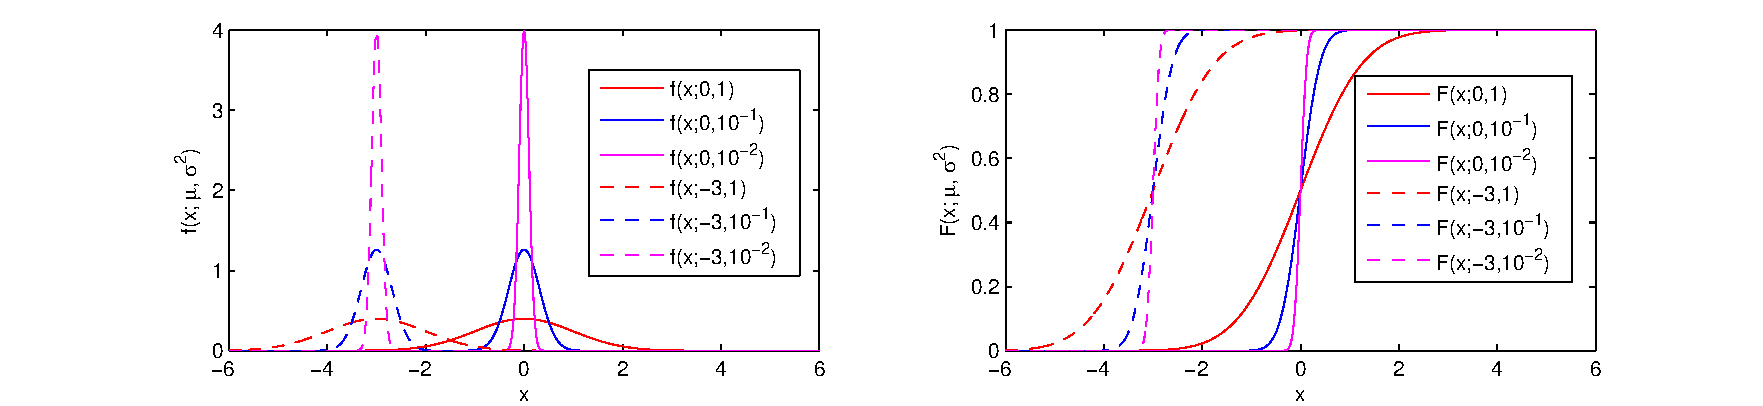
\includegraphics[width=6.5in]{figures/plotPdfCdfNormals}}
\end{figure}

\paragraph{Mean and Variance of $\normal(\mu,\sigma^2)$:}
The mean of a $\normal(\mu,\sigma^2)$ RV $X$ is:
\[
\e(X) = \int_{-\infty}^{\infty} x f(x;\mu,\sigma^2)\,dx
=   \frac{1}{\sigma \sqrt{2 \pi}} \int_{-\infty}^{\infty} x
 \exp{\left( - \frac{1}{2 \sigma^2} (x-\mu)^2 \right)}\,dx
= \mu \ ,
\]
and the variance is:
\[
\V(X) = \int_{-\infty}^{\infty} (x-\mu)^2 f(x;\mu,\sigma^2)\,dx
=   \frac{1}{\sigma \sqrt{2 \pi}} \int_{-\infty}^{\infty} (x-\mu)^2
 \exp{\left( - \frac{1}{2 \sigma^2} (x-\mu)^2 \right)}\,dx
= \sigma^2 \ .
\]

%\remove{
\begin{labwork}[Compute the  the $\p(X \in (a,b))$ for the $\normal(0,1)$ RV $X$]\label{LW:NormalIntervalProb}
Write a function to evaluate the $\p(X \in (a,b))$ for the $\normal(0,1)$ RV $X$ for user-specified values of $a$ and $b$. [Hint: one option is by making two calls to {\tt NormalCdf} and doing one arithmetic operation.]
\end{labwork}

Simulations \ref*{SIM:Uniformab} and \ref*{SIM:Exponential}, \ref*{SIM:Laplace} and \ref*{SIM:StdCauchy}
produce samples from a continuous RV $X$ with a closed-form expression for the inverse DF $F^{[-1]}$ via \hyperref[A:InvS]{Algorithm~\ref*{A:InvS}} (\hyperref[T:ContinRVsInvS]{Table~\ref*{T:ContinRVsInvS}}).  But only a few RVs have an explicit $F^{[-1]}$.  For example, $\normal(0,1)$ RV does not have an explicit $F^{[-1]}$.
\hyperref[A:InvSbyNumSol]{Algorithm~\ref*{A:InvSbyNumSol}} is a more general but inexact method that relies on an approximate numerical solution of $x$, for a given $u$, that satisfies the equation $F(x)=u$.

\begin{algorithm}
\caption{ Inversion Sampler by Numerical Solution of $F(X)=U$ via Newton-Raphson Method}
\label{A:InvSbyNumSol}
\begin{algorithmic}[1]
\STATE {{\it input:} $F(x)$, the DF of the target RV $X$}
\STATE {{\it input:} $f(x)$, the density of $X$}
%\STATE {{\it input:} The fundamental sampler}
\STATE {{\it input:} A reasonable {\tt Stopping Rule}, \\e.g.~a specified tolerance $\epsilon >0$ and a maximum number of iterations {\tt MAX}}
\STATE {{\it input:} a careful mechanism to specify $x_0$}
%\STATE {\it initialise:} set the seed, if any, for the fundamental sampler
\STATE {\it output:} a sample from $X$ distributed according to $F$
\STATE {{\it draw:} $u \sim \uniform(0,1)$}
\STATE{{\it initialise:} $i \gets 0, \qquad x_i \gets x_0, \qquad x_{i+1} \gets x_0 - \frac{F(x_0)-u}{f(x_0)}$}
\WHILE{{\tt Stopping Rule} is not satisfied,\\e.g.~$|F(x_{i})-F(x_{i-1})| > \epsilon$ AND $i < {\tt MAX}$}
\STATE $x_i \gets x_{i+1}$
\STATE $x_{i+1} \gets \left( x_{i} - \frac{F(x_i)-u}{f(x_i)} \right)$
\STATE $i \gets i+1$
\ENDWHILE
\STATE{{\it return:} $x \gets x_i$}
\end{algorithmic}
\end{algorithm}

\begin{simulation}[$\normal(\mu,\sigma^2)$]\label{SIM:NormalByNewRap}
We may employ \hyperref[A:InvSbyNumSol]{Algorithm~\ref*{A:InvSbyNumSol}} to sample from the $Normal(\mu,\sigma^2)$ RV $X$ using the following function.
 \VrbMf[label=Sample1NormalByNewRap.m]{scripts/Sample1NormalByNewRap.m}

We draw five samples from the $\normal(0,1)$ RV $Z$ and store them in $z$ as follows.  The vector $z$ can be obtained by a Newton-Raphson-based numerical transformation of the vector $u$ of $5$ IID samples from the $\uniform(0,1)$ RV.  We simply need to apply the function {\tt Sample1NormalByNewRap} to each element of an array of $\uniform(0,1)$ samples.  \Matlab's {\tt arrayfun} command can be used to apply {\tt @(u)(Sample1NormalByNewRap(u,0,1))} (i.e., {\tt Sample1NormalByNewRap} as a function of $u$) to every element of our array of $\uniform(0,1)$ samples, say {\tt Us}.  Note that $F(z)$ is the same as the drawn $u$ from $U$ at least up to four significant digits.
\begin{VrbM}
>> rand('twister',563987);
>> Us=rand(1,5); % store 5 samples from Uniform(0,1) RV in array Us
>> disp(Us); % display Us
    0.8872    0.2569    0.5275    0.8650    0.8517
>> z=Sample1NormalByNewRap(Us(1),0,1); %transform Us(1) to a Normal(0,1) sample z
>> disp(z); % display z
    1.2119
>> z = arrayfun(@(u)(Sample1NormalByNewRap(u,0,1)),Us); %transform array Us via arrayfun
>> % dislay array z obtained from applying Sample1NormalByNewRap to each element of Us
>> disp(z);
    1.2119   -0.6530    0.0691    1.1031    1.0439
>> % check that numerical inversion of F worked, i.e., is F(z)=u ?
>> disp(NormalCdf(z,0,1));
    0.8872    0.2569    0.5275    0.8650    0.8517
\end{VrbM}
Next we draw five samples from the $\normal(-100.23,0.01)$ RV $X$, store it in an array $x$ and observe that the numerical method is reasonably accurate by the equality of $u$ and $F(x)$.
\begin{VrbM}
>> rand('twister',563987);
>> disp(Us); % display Us
    0.8872    0.2569    0.5275    0.8650    0.8517
>> % transform array Us via arrayfun
>> x = arrayfun(@(u)(Sample1NormalByNewRap(u,-100.23,0.01)),Us);
>> disp(x);
 -100.1088 -100.2953 -100.2231 -100.1197 -100.1256
>> disp(NormalCdf(x,-100.23,0.01));
    0.8872    0.2569    0.5275    0.8650    0.8517
\end{VrbM}
One has to be extremely careful with this approximate simulation algorithm implemented in floating-point arithmetic.  More robust samplers for the $\normal(\mu,\sigma^2)$ RV exist.
However, \hyperref[A:InvSbyNumSol]{Algorithm~\ref*{A:InvSbyNumSol}} is often the only choice when simulating from an arbitrary RV with an unknown closed-form expression for its $F^{[-1]}$.
\end{simulation}
%%% begin of informal CLT excursion
Next, we use our simulation capability to gain an informal and intuitive understanding of one of the most elementary theorems in probability and statistics, namely, the Central Limit Theorem (CLT).  We will see a formal treatment of CLT later.

Informally, the CLT can be stated as follows:\\
``The sample mean of a large number of IID samples, none of which is dominant, tends to the $\normal$ distribution as the number of samples increases.''

\begin{labwork}[Investigating the Central Limit Theorem with IID $\exponential(\lambda=0.1)$ RVs]\label{LW:CLTOfExponentials}
Let us investigate the histograms from $10000$ simulations of the sample mean of $n=10,100,1000$ IID $\exponential(\lambda=0.1)$ RVs as follows:
\begin{VrbM}
>> rand('twister',1973); % initialise the fundamental sampler
>> % a demonstration of Central Limit Theorem (CLT) -- Details of CLT are in the sequel
>> % the sample mean should be a Normal(1/lambda,lambda/n) RV
>> lambda=0.1; Reps=10000; n=10; hist(sum(-1/lambda * log(rand(n,Reps)))/n)
>> lambda=0.1; Reps=10000; n=100; hist(sum(-1/lambda * log(rand(n,Reps)))/n,20)
>> lambda=0.1; Reps=10000; n=1000; hist(sum(-1/lambda * log(rand(n,Reps)))/n,20)
\end{VrbM}
Do you see a pattern in the histograms?

See the histograms generated from the following code that produces sample means from the $\cauchy$ RV:
\begin{VrbM}
>> Reps=10000; n=1000; hist(sum(tan(pi * rand(n,Reps)))/n,20)
>> Reps=10000; n=1000; hist(sum(tan(pi * rand(n,Reps)))/n,20)
>> Reps=10000; n=1000; hist(sum(tan(pi * rand(n,Reps)))/n,20)
\end{VrbM}
\end{labwork}
\begin{classwork}[Why doesn't the sample mean of the $\cauchy$ RV ever settle down?]
Explain in words why the mean of $n$ IID samples from the $\cauchy$ RV ``is {\bf not} obeying'' the Central Limit Theorem.  Also relate it to \hyperref[F:plot5RunningMeansStandardcauchyUnif010]{Figure~\ref*{F:plot5RunningMeansStandardcauchyUnif010}} of \hyperref[LW:RunningMeanCauchy]{Labwork~\ref*{LW:RunningMeanCauchy}}.
\end{classwork}
%}% end remove

\begin{model}[$\gammA(\lambda,k)$ RV]
Given a shape parameter $\alpha>0$ and a rate parameter $\beta>0$, the RV $X$ is said to be $\gammA(\alpha,\beta)$ distributed if its PDF is:
\[
f(x;\alpha,\beta) = \frac{\beta^{\alpha}}{\Gamma(\alpha)} x^{\alpha-1} \exp(-\beta x), \qquad x > 0 \ ,
\]
where, the gamma function which interpolates the factorial function is:
\[
\Gamma(\alpha) := \int_0^{\infty} \exp(-y) y^{\alpha-1} dy \ .
\]
When $k \in \Nz$, then $\Gamma(k)=(k-1)!$.  The DF of $X$ is:
\[
F(x;\lambda,k) = \BB{1}_{\Rz_{>0}}(x) \frac{\beta^{\alpha}}{\Gamma(\alpha)} \int_0^{x} y^{\alpha-1} \exp(-\beta y) dy =
\begin{cases}
0 & \text{if } x \leq 0 \\
 \frac{\gamma(\alpha,\beta x)}{\Gamma(\alpha)} & \text{if } x > 0
\end{cases}
\]
where $\gamma(\alpha,\beta x)$ is called the lower incomplete Gamma function.
\end{model}
The expectation and variance of a $\gammA(\alpha,\beta)$ RV are $\alpha/\beta$ and $\alpha/\beta^2$, respectively.
%\remove{
The Gamma function and the incomplete Gamma function are available as \Matlab functions {\tt gamma} and {\tt gammainc}, respectively.  Thus, {\tt gamma(k)} returns $\Gamma(k)$ and {\tt gammainc(lambda*x,k)} returns $F({\tt x};{\tt lambda},{\tt k})$.  Using these functions, it is straightforward to evaluate the PDF and CDF of $X \sim \gammA(\lambda,k)$.  We use the following script to get a sense for the impact upon the PDF and CDF of the shape parameter $k$ as it ranges in $\{1,2,3,4,5\}$ for a given scale parameter $\lambda=0.1$.
\VrbMf[label=PlotPdfCdfGamma.m]{scripts/PlotPdfCdfGamma.m}
%}%end remove

\begin{figure}[htpb]
\caption{PDF and CDF of $X \sim \gammA(\beta=0.1,\alpha)$ with $\alpha \in \{1,2,3,4,5\}$.\label{F:PlotPdfCdfGamma}}
\centering   \makebox{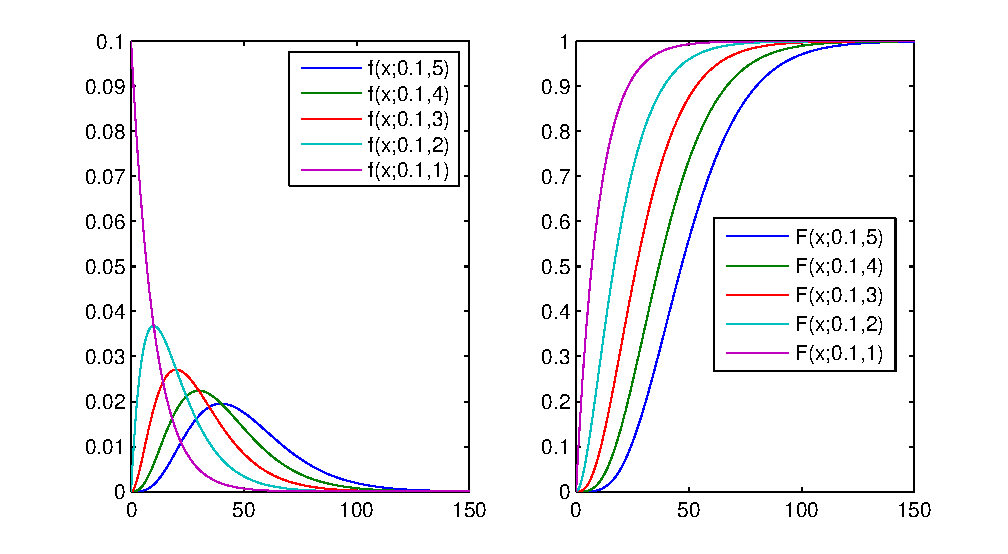
\includegraphics[width=6.50in]{figures/PlotPdfCdfGamma}}
\end{figure}


Note that if $X \sim \gammA(1,\beta)$ then $X \sim \exponential(\beta)$, since:
\[
f(x;1,\beta)  
= \frac{1}{(1-1)!}  \beta \exp(-\beta x) = \beta \exp(-\beta x) \ .
\]
More generally, if $X \sim \gammA(\alpha,\beta)$ and $\alpha \in \Nz$, then $X \sim \sum_{i=1}^{\alpha} Y_i$, where $Y_i \overset{IID}{\sim} \exponential(\beta)$ RVS, i.e.~ the sum of $\alpha$ IID $\exponential(\beta)$ RVs forms the model for the $\gammA(\alpha,\beta)$ RV.  If you model the inter-arrival time of buses at a bus-stop by IID $\exponential(\beta)$ RV, then you can think of the arrival time of the $k^{\text th}$ bus as a $\gammA(\alpha,\beta)$ RV.

\section{Discrete Random Variables}

%\remove{
\section{Inversion Sampler for Discrete Random Variables}\label{S:InvSDiscrete}
Next, consider the problem of {\bf sampling from a random variable $X$ with a discontinuous or discrete DF} using the inversion sampler.  We need to define the inverse more carefully here.
\begin{prop}[Inversion sampler with compact support]
Let the support of the RV $X$ be over some real interval $[a,b]$ and let its inverse DF be defined as follows:
\[
F^{[-1]}(u) := \inf\{ x \in [a,b]: F(x) \geq u, \ 0 \leq u \leq 1 \} \ .
\]
If $U \sim \uniform(0,1)$ then $F^{[-1]}(U)$ has the DF $F$, i.e.~$F^{[-1]}(U) \sim F \sim X$.
\end{prop}
\begin{proof}
The proof is a consequence of the following equalities:
\[
\p(F^{[-1]}(U) \leq x) = \p(U \leq F(x)) = F(x) := \p(X \leq x)
\]
\end{proof}

\section{Some Simulations of Discrete Random Variables}\label{S:InvSDiscreteRVs}

\begin{simulation}[$\bernoulli(\theta)$]\label{SIM:Bernoulli}
Consider the problem of simulating from a $\bernoulli(\theta)$ RV based on an input from  a $\uniform(0,1)$ RV.  Recall that $\lfloor x \rfloor$ (called the `floor of $x$') is the largest integer that is smaller than or equal to $x$, e.g.~$\lfloor 3.8 \rfloor = 3$.  Using the floor function, we can simulate a $\bernoulli(\theta)$ RV $X$ as follows:
\begin{VrbM}
>>  theta = 0.3;		% set theta = Prob(X=1)
  % return x  -- floor(y) is the largest integer less than or equal to y
>> x = floor(rand + theta)	% rand is the Fundamental Sampler
>> disp(x) % display the outcome of the simulation
     0
>> n=10;  % set the number of IID Bernoulli(theta=0.3) trials you want to simulate
>> x = floor(rand(1,10)+theta); % vectorize the operation
>> disp(x) % display the outcomes of the simulation
     0     0     1     0     0     0     0     0     1     1
\end{VrbM}
\end{simulation}
Again, it is straightforward to do replicate experiments, e.g.~to demonstrate the Central Limit Theorem for a sequence of $n$ IID $\bernoulli(\theta)$ trials.
\begin{VrbM}
>> % a demonstration of Central Limit Theorem --
>> % the sample mean of a sequence of n IID Bernoulli(theta) RVs is Gaussian(theta,theta(1-theta)/n)
>> theta=0.5; Reps=10000; n=10; hist(sum(floor(rand(n,Reps)+theta))/n)
>> theta=0.5; Reps=10000; n=100; hist(sum(floor(rand(n,Reps)+theta))/n,20)
>> theta=0.5; Reps=10000; n=1000; hist(sum(floor(rand(n,Reps)+theta))/n,30)
\end{VrbM}

Consider the class of discrete RVs with distributions that place all probability mass on a single real number.  This is the probability model for the  deterministic real variable.
\begin{model}[$\pointmass(\theta)$]
Given a specific point $\theta \in \Rz$, we say an RV $X$ has point mass at $\theta$ or is $\pointmass(\theta)$ distributed if the DF is:
\begin{equation}\label{E:PointMasscdf}
F(x;\theta) =
\begin{cases}
0 & \text{if $x < \theta$} \\
1 & \text{if $x \geq \theta$}
\end{cases}
\end{equation}
and the PMF is:
\begin{equation}
f(x;\theta) =
\begin{cases}
0 & \text{if  $x \neq \theta$} \\
1 & \text{if $x = \theta$}
\end{cases}
\end{equation}
\end{model}
Thus, $\pointmass(\theta)$ RV $X$ is deterministic in the sense that every realisation of $X$ is exactly equal to $\theta \in \Rz$.  We will see that this distribution plays a central limiting role in asymptotic statistics.
\paragraph{Mean and variance of $\pointmass(\theta)$ RV:}
Let $X \sim \pointmass(\theta)$.  Then:
\[
\e(X) = \sum_{x} x f(x) = \theta \times 1 = \theta \ , \qquad
\V(X) = \e(X^2) - (\e(X))^2 = \theta^2 - \theta^2 = 0 \ .
\]
\begin{simulation}[$\pointmass(\theta)$]\label{SIM:PointMass}
Let us simulate a sample from the $\pointmass(\theta)$ RV $X$.  Since this RV produces the same realisation $\theta$ we can implement it via the following M-file:

\VrbMf[label=Sim1PointMass.m]{scripts/Sim1PointMass.m}
Here is call to the function.
\begin{VrbM}
>> Sim1PointMass(rand(),2)
ans =     2
>> % % we can use arrayfun to apply Sim1Pointmass to any array of Uniform(0,1) samples
>> arrayfun(@(u)(Sim1PointMass(u,17)),rand(2,10))
ans =
    17    17    17    17    17    17    17    17    17    17
    17    17    17    17    17    17    17    17    17    17
\end{VrbM}
Note that it is not necessary to have input IID samples from $\uniform(0,1)$ RV via {\tt rand} in order to draw samples from the $\pointmass(\theta)$ RV.  For instance, an input matrix of zeros can do the job:
\begin{VrbM}
>> arrayfun(@(u)(Sim1PointMass(u,17)),zeros(2,8))
ans =
    17    17    17    17    17    17    17    17
    17    17    17    17    17    17    17    17
\end{VrbM}
\end{simulation}


Next let us consider a natural generalization of the $\bernoulli(\theta)$ RV with more than two outcomes.
\begin{model}[{$\demoivre(\theta_1,\theta_2,\ldots,\theta_k)$}]\label{M:deMoivre}
Given a specific point $(\theta_1,\theta_2,\ldots,\theta_k)$ in the $k$-Simplex:
\[
\bigtriangleup_k :=  \{ \,  ( \theta_1,\theta_2,\ldots,\theta_k) :  \theta_1 \geq 0, \theta_2 \geq 0, \ldots, \theta_k \geq 0, \sum_{i=1}^k \theta_i = 1 \, \}  \ ,
\]
we say that an RV $X$ is $\demoivre(\theta_1,\theta_2,\ldots,\theta_k)$ distributed if its PMF is:
\[
f(x;\theta_1,\theta_2,\ldots,\theta_k) =
\begin{cases}
0 & \quad \text{if $x \notin [k] := \{1,2,\ldots,k\}$,} \\
\theta_x & \quad \text{if $x \in [k]$}   .
\end{cases}
\]
The DF for $\demoivre(\theta_1,\theta_2,\ldots,\theta_k)$ RV $X$ is:
\begin{equation}\label{E:deMoivreDF}
F(x;\theta_1,\theta_2,\ldots,\theta_k) =
\begin{cases}
0 & \quad  \text{if $-\infty < x < 1$}\\
\theta_1 & \quad \text{if $1 \leq x < 2$} \\
\theta_1+\theta_2 & \quad \text{if $2 \leq x < 3$} \\
\vdots & \\
\theta_1+\theta_2+\cdots+\theta_{k-1} & \quad \text{if $k-1 \leq x < k$} \\
\theta_1+\theta_2+\cdots+\theta_{k-1}+\theta_k=1 & \quad \text{if $k \leq x < \infty$} \\
\end{cases}
\end{equation}
The $\demoivre(\theta_1,\theta_2,\ldots,\theta_k)$ RV can be thought of as a probability model for ``the outcome  of rolling a polygonal cylindrical die with $k$ rectangular faces that are marked with $1, 2, \ldots, k$''.  The parameters $\theta_1,\theta_2,\ldots,\theta_k$ specify how the die is loaded and may be idealised as specifying the cylinder's centre of mass with respect to the respective faces.  Thus, when $\theta_1=\theta_2=\cdots=\theta_k=1/k$, we have a probability model for the outcomes of a fair die.
\end{model}

\paragraph{Mean and variance of $\demoivre (\theta_1,\theta_2,\ldots,\theta_k)$ RV:}
The not too useful expressions for the first two moments of $X \sim \demoivre (\theta_1,\theta_2,\ldots,\theta_k)$ are,
\[
\e(X) = \sum_{x=1}^k x \theta(x) =  \theta_1 + 2 \theta_2 + \cdots + k \theta_k \ , \text{ and }
\]
\[
\V(X) = \e(X^2) - (\e(X))^2 =   \left(\theta_1 + 2^2 \theta_2 + \cdots + k^2 \theta_k \right) - \left( \theta_1 + 2 \theta_2 + \cdots + k \theta_k \right)^2 \ .
\]
However, if $X\sim \demoivre(1/k,1/k,\ldots,1/k)$, then the mean and variance for the fair $k$-faced die based on Faulhaber's formula for $\sum_{i=1}^k i^m$, with $m\in\{1,2\}$, are,
\[
\e(X) = \frac{1}{k} \left( 1+2+\cdots+k \right)= \frac{1}{k} \frac{k(k+1)}{2} = \frac{k+1}{2}  \ ,
\]
\[
\e(X^2) = \frac{1}{k} \left( 1^2+2^2+\cdots+k^2 \right)  = \frac{1}{k} \frac{k(k+1)(2k+1)}{6} =  \frac{2k^2+3k+1}{6} \ ,
\]
\begin{align}
\V(X) = \e(X^2) - (\e(X))^2
&= \frac{2k^2+3k+1}{6} -  \left( \frac{k+1}{2} \right)^2 = \frac{2k^2+3k+1}{6} -  \left( \frac{k^2+2k+1}{4} \right) \notag \\
&=  \frac{8k^2+12k+4 - 6k^2-12k-6}{24} =  \frac{2k^2-2}{24} = \frac{k^2-1}{12} \notag \ .
\end{align}

Next we simulate from $\demoivre(\theta_1,\theta_2,\ldots,\theta_k)$ RV $X$ via its inverse DF $$F^{[-1]}: [0,1] \rightarrow [k] := \{1,2,\ldots,k\} \ ,$$ given by:
\begin{equation}\label{E:deMoivreInverseDF}
F^{[-1]}(u;\theta_1,\theta_2,\ldots,\theta_k) =
\begin{cases}
1 & \quad \text{if $0 \leq u < \theta_1$}\\
2 & \quad \text{if $\theta_1 \leq u < \theta_1+\theta_2$} \\
3 & \quad \text{if $\theta_1+\theta_2 \leq u < \theta_1+\theta_2+\theta_3$} \\
\vdots & \\
k & \quad \text{if $\theta_1+\theta_2+\cdots+\theta_{k-1} \leq u < 1$} \\
\end{cases}
\end{equation}
When $k=2$ in the $\demoivre(\theta_1,\theta_2)$ model, we have an RV that is similar to the $\bernoulli(p=\theta_1)$ RV.  The DF $F$ and its inverse $F^{[-1]}$ for a specific $\theta_1=0.3$ are depicted in \hyperref[F:InvSamk2]{Figure \ref*{F:InvSamk2}}.

\begin{figure}[htpb]
\caption{The DF $F(x;0.3,0.7)$ of the $\demoivre(0.3,0.7)$ RV and its inverse $F^{[-1]}(u;0.3,0.7)$. \label{F:InvSamk2}}
\centering   \makebox{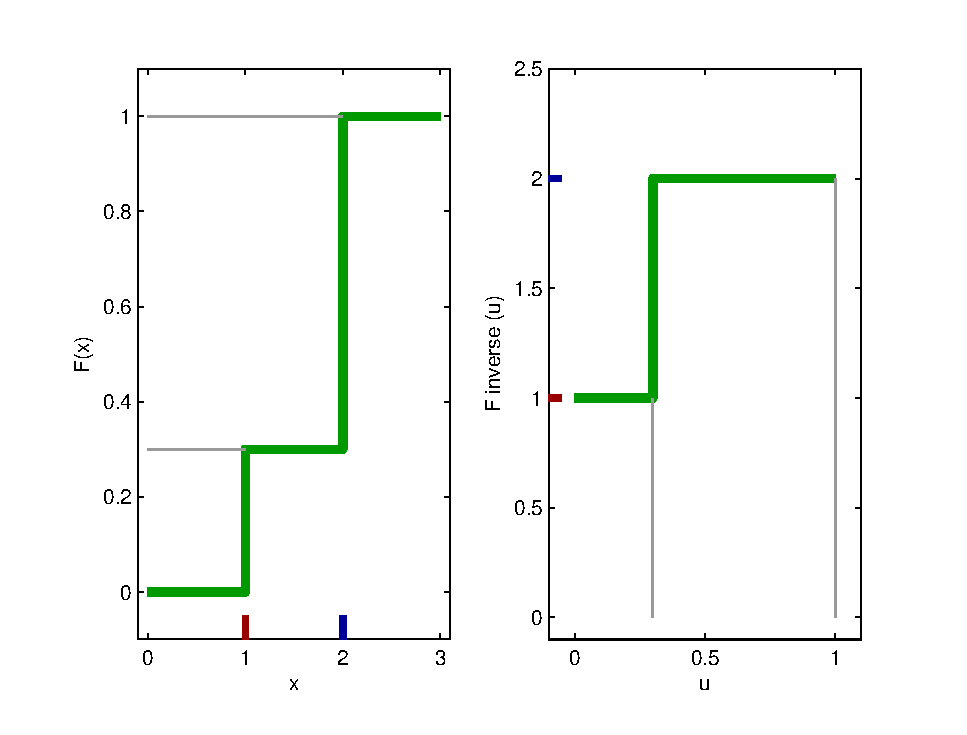
\includegraphics[width=10cm]{figures/plotInvSamk2R}}
\end{figure}

First we simulate from an equi-probable special case of the $\demoivre(\theta_1,\theta_2,\ldots,\theta_k)$ RV, with $\theta_1=\theta_2=\cdots=\theta_k=1/k$.
\begin{simulation}[$\demoivre(1/k,1/k,\ldots,1/k)$]\label{SIM:deMoivreEqui}
The equi-probable $de~Moivre(1/k,1/k,\ldots,1/k)$ RV $X$ with a discrete uniform distribution over $[k] = \{1,2,\ldots k\}$ can be efficiently sampled using the ceiling function.  Recall that $\lceil y \rceil$ is the smallest integer larger than or equal to $y$, eg.~$\lceil 13.1 \rceil = 14$.  \hyperref[A:SimdeMoivreEqui]{Algorithm~\ref*{A:SimdeMoivreEqui}} produces samples from the $de~Moivre(1/k,1/k,\ldots,1/k)$ RV $X$.

\begin{algorithm}[h]
\caption{ Inversion Sampler  for $\demoivre(1/k,1/k,\ldots,1/k)$ RV}
\label{A:SimdeMoivreEqui}
\begin{algorithmic}[1]
\STATE {
{\it input:}
\begin{enumerate}
\item $k$ in $\demoivre(1/k,1/k,\ldots,1/k)$ RV $X$
\item $u \sim \uniform(0,1)$
\end{enumerate}
}
\STATE {\it output:} a sample from $X$
\STATE {{\it return:} $x \gets \lceil k u \rceil $}
\end{algorithmic}
\end{algorithm}

The M-file implementing \hyperref[A:SimdeMoivreEqui]{Algorithm~\ref*{A:SimdeMoivreEqui}} is:
 \VrbMf[label=SimdeMoivreEqui.m]{scripts/SimdeMoivreEqui.m}
Let us use the function {\tt SimdeMoivreEqui} to draw five samples from a fair seven-faced cylindrical dice.
\begin{VrbM}
>> k=7; % number of faces of the fair dice
>> n=5; % number of trials
>> rand('twister',78657); % initialise the fundamental sampler
>> u=rand(1,n); % draw n samples from Uniform(0,1)
>> % inverse transform samples from Uniform(0,1) to samples
>> % from de Moivre(1/7,1/7,1/7,1/7,1/7,1/7,1/7)
>> outcomes=SimdeMoivreEqui(u,k); % save the outcomes in an array
>> disp(outcomes);
     6     5     5     5     2
\end{VrbM}
\end{simulation}

Now, let us consider the more general problem of implementing a sampler for an arbitrary but specified $\demoivre(\theta_1,\theta_2,\ldots,\theta_k)$ RV.  That is, the values of $\theta_i$ need not be equal to $1/k$.
\begin{simulation}[$\demoivre(\theta_1,\theta_2,\ldots,\theta_k)$]\label{SIM:deMoivre}
We can generate samples from a $\demoivre(\theta_1,\theta_2,\ldots,\theta_k)$ RV $X$ when $(\theta_1,\theta_2,\ldots,\theta_k)$ are specifiable as an input vector via the following algorithm.

\begin{algorithm}
\caption{Inversion Sampler for $\demoivre(\theta_1,\theta_2,\ldots,\theta_k)$ RV $X$}
\label{A:SimdeMoivre}
\begin{algorithmic}[1]
\STATE {
{\it input:}
\begin{enumerate}
\item parameter vector $(\theta_1,\theta_2,\ldots,\theta_k)$ of $\demoivre(\theta_1,\theta_2,\ldots,\theta_k)$ RV $X$.
\item $u \sim \uniform(0,1)$
\end{enumerate}
}
\STATE {\it output:} a sample from $X$
\STATE {\it initialise:}  $F \gets \theta_1$, $i \gets 1$
\WHILE{$u > F$}
\STATE $i \gets i+1$
\STATE $F \gets F+\theta_{i}$
\ENDWHILE
\STATE {\it return:} $x \gets i$
\end{algorithmic}
\end{algorithm}

The M-file implementing \hyperref[A:SimdeMoivre]{Algorithm~\ref*{A:SimdeMoivre}} is:
 \VrbMf[label=SimdeMoivreOnce.m]{scripts/SimdeMoivreOnce.m}
Let us use the function {\tt deMoivreEqui} to draw five samples from a fair seven-faced dice.
\begin{VrbM}
>> k=7; % number of faces of the fair dice
>> n=5; % number of trials
>> rand('twister',78657); % initialise the fundamental sampler
>> Us=rand(1,n); % draw n samples from Uniform(0,1)
>> disp(Us);
    0.8330    0.6819    0.6468    0.6674    0.2577
>> % inverse transform samples from Uniform(0,1) to samples
>> % from de Moivre(1/7,1/7,1/7,1/7,1/7,1/7,1/7)
>> f=[1/7 1/7 1/7 1/7 1/7 1/7 1/7];
>> disp(f);
    0.1429    0.1429    0.1429    0.1429    0.1429    0.1429    0.1429
>> % use funarray to apply function-handled SimdeMoivreOnce to
>> % each element of array Us and save it in array outcomes2
>> outcomes2=arrayfun(@(u)(SimdeMoivreOnce(u,f)),Us);
>> disp(outcomes2);
     6     5     5     5     2
>> disp(SimdeMoivreEqui(u,k)); % same result using the previous algorithm
     6     5     5     5     2
\end{VrbM}
Clearly, \hyperref[A:SimdeMoivre]{Algorithm~\ref*{A:SimdeMoivre}} may be used to sample from any $\demoivre(\theta_1,\ldots,\theta_k)$ RV $X$.  We demostrate this by producing five samples from a randomly generated PMF {\tt f2}.
\begin{VrbM}
>> rand('twister',1777); % initialise the fundamental sampler
>> f2=rand(1,10); % create an arbitrary array
>> f2=f2/sum(f2); % normalize to make a probability mass function
>> disp(f2); % display the weights of our 10-faced die
    0.0073    0.0188    0.1515    0.1311    0.1760    0.1121    ...
    0.1718    0.1213    0.0377    0.0723
>> disp(sum(f2)); % the weights sum to 1
    1.0000
>> disp(arrayfun(@(u)(SimdeMoivreOnce(u,f2)),rand(5,5))) % the samples from f2 are
     4     3     4     7     3
     6     7     4     5     3
     5     8     7    10     6
     2     3     5     7     7
     6     5     9     5     7
\end{VrbM}
\end{simulation}

Note that the principal work here is the sequential search, in which the mean number of comparisons until success is:
\[
1 \theta_1 + 2 \theta_2 + 3 \theta_3 + \ldots + k \theta_k = \sum_{i=1}^k{ i \theta_i}
\]
For the $\demoivre(1/k,1/k,\ldots,1/k)$ RV, the right-hand side of the above expression is:
\[
\sum_{i=1}^k{ i \frac{1}{k}} = \frac{1}{k} \sum_{i=1}^k{ i} = \frac{1}{k} \frac{k(k+1)}{2} = \frac{k+1}{2} \ ,
\]
indicating that the average-case efficiency is linear in $k$.  This linear dependence on $k$ is denoted by $O(k)$.  In other words, as the number of faces $k$ increases, one has to work linearly harder to get samples from $\demoivre(1/k,1/k,\ldots,1/k)$ RV using \hyperref[A:SimdeMoivre]{Algorithm \ref*{A:SimdeMoivre}}.  Using the simpler \hyperref[A:SimdeMoivreEqui]{Algorithm \ref*{A:SimdeMoivreEqui}}, which exploits the fact that all values of $\theta_i$  are equal, we generated samples in constant time, which is denoted by $O(1)$.
%}%end remove
Let us consider a RV that arises from an IID stochastic process of $\bernoulli(\theta)$ RVs $\{X_i\}_{i \in \Nz}$, ie.~
\[
 \{X_i\}_{i \in \Nz} := \{X_1, X_2,\ldots\}  \overset{\IID}{\sim} \bernoulli(\theta) \ .
\]
When we consider the number of IID $\bernoulli(\theta)$ trials before the first `Head' occurs we get the following discrete RV.
\begin{model}[$\geometric(\theta)$ RV]
Given a parameter $\theta \in (0,1)$, the PMF of the $\geometric(\theta)$ RV $X$ is
\begin{equation}\label{E:Geometricpdf}
f(x;\theta) =
\begin{cases}
\theta(1-\theta)^{x} & \text{if $x \in \Zz_+ := \{0,1,2,\ldots \}$} \\
0 & \text{otherwise}
\end{cases}
\end{equation}
It is straightforward to verify that $f(x;\theta)$ is indeed a PDF :
\[
\sum_{x=0}^{\infty} f(x;\theta) = \sum_{x=0}^{\infty} \theta(1-\theta)^{x}
= \theta \left( \frac{1}{1-(1-\theta)} \right) =  \theta \left( \frac{1}{\theta} \right) = 1
\]

{\scriptsize
The above equality is a consequence of the geometric series identity \eqref{E:GeomSeries} with $a=\theta$ and $\vartheta:=1-\theta$:
\begin{equation}\label{E:GeomSeries}
 \sum_{ x =0}^{\infty} a \vartheta^x = a \left( \frac{1}{1-\vartheta} \right) , \ \text{provided, } 0 < \vartheta < 1 \ .
\end{equation}
\begin{proof}
\[
a+a\vartheta+a\vartheta^2+\cdots+a\vartheta^n
= \sum_{0 \leq x \leq n} a \vartheta^x
= a+ \sum_{1 \leq x \leq n} a \vartheta^x
= a +  \vartheta  \sum_{1 \leq x \leq n} a \vartheta^{x-1}
= a +  \vartheta  \sum_{0 \leq x \leq n-1} a \vartheta^{x}
= a +  \vartheta  \sum_{0 \leq x \leq n} a \vartheta^{x} - a \vartheta^{n+1}
\]
Therefore,
\begin{eqnarray}
\sum_{0 \leq x \leq n} a \vartheta^x
&=&  a +  \vartheta  \sum_{0 \leq x \leq n} a \vartheta^{x} - a \vartheta^{n+1} \notag \\
\left( \sum_{0 \leq x \leq n} a \vartheta^x \right) - \left( \vartheta  \sum_{0 \leq x \leq n} a \vartheta^{x} \right)
&=&  a  - a \vartheta^{n+1} \notag \\
\left( \sum_{0 \leq x \leq n} a \vartheta^x \right) (1-\vartheta)
&=&  a (1 -  \vartheta^{n+1}) \notag \\
\sum_{0 \leq x \leq n} a \vartheta^x
&=&  a \left( \frac{1 -  \vartheta^{n+1}}{1-\vartheta} \right) \notag\\
 \sum_{ x =0}^{\infty} a \vartheta^x  := \lim_{n \rightarrow \infty} \sum_{0 \leq x \leq n} a \vartheta^x
&=&  a \left( \frac{1}{1-\vartheta} \right) , \ \text{provided, } 0 < \vartheta < 1 \notag
\end{eqnarray}
\end{proof}
}
The outcome of a $\geometric(\theta)$ RV can be thought of as ``the number of tosses needed before the appearance of the first `Head' when tossing a coin with probability of `Heads' equal to $\theta$ in a independent and identical manner.''
\end{model}

\paragraph{Mean and variance of $\geometric(\theta)$ RV:}
Let $X \sim \geometric(\theta)$ RV.  Then,
\[
\e(X) = \sum_{x=0}^{\infty} x \theta(1-\theta)^x =  \theta \sum_{x=0}^{\infty} x (1-\theta)^x
\]
In order to simplify the RHS above, let us employ differentiation with respect to $\theta$:
\[
\frac{-1}{\theta^2}= \frac{d}{d\theta} \left( \frac{1}{\theta} \right)= \frac{d}{d\theta} \sum_{x=0}^{\infty} (1-\theta)^x  =  \sum_{x=0}^{\infty} -x (1-\theta)^{x-1}
\]
Multiplying the LHS and RHS above by $-(1-\theta)$ and substituting in $\e(X)=  \theta \sum_{x=0}^{\infty} x (1-\theta)^x$, we get a much simpler expression for $\e(X)$ :
\[
\frac{1-\theta}{\theta^2}= \sum_{x=0}^{\infty} x (1-\theta)^{x} \implies \e(X) = \theta \left( \frac{1-\theta}{\theta^2} \right) = \frac{1-\theta}{\theta} \ .
\]
Similarly, it can be shown that
\[
\V(X) = \frac{1-\theta}{\theta^2} \ .
\]

\begin{figure}[htpb]
\caption{Mean and variance of a $\geometric(\theta)$ RV $X$ as a function of the parameter $\theta$.\label{F:MeanVarGeom}}
\centering   \makebox{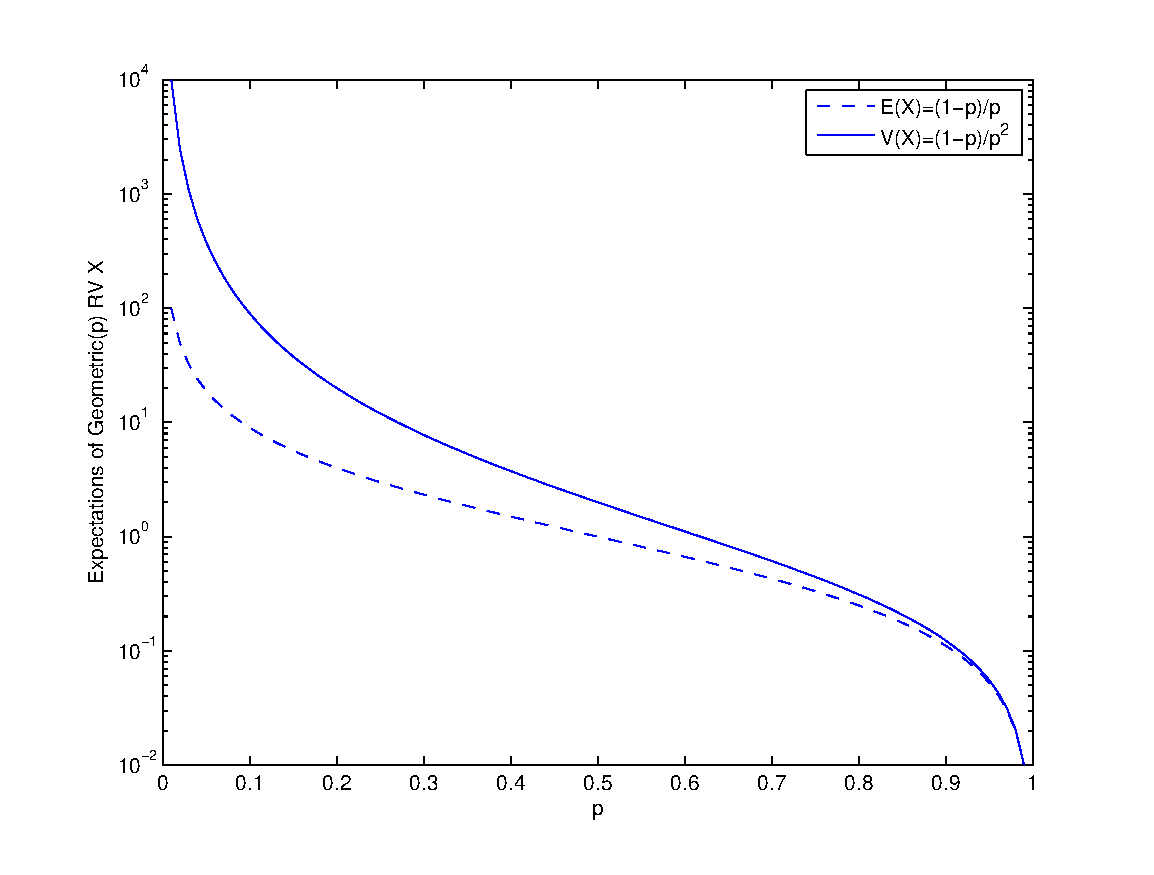
\includegraphics[width=5.0in]{figures/PlotMeanVarGeom}}
\end{figure}

%\remove{
\begin{simulation}[$\geometric(\theta)$]\label{SIM:Geometric}
We can simulate a sample $x$ from a $\geometric(\theta)$ RV $X$ using the following simple algorithm:
\[
x \gets \lfloor \log(u) / \log(1-\theta) \rfloor, \qquad \text{where, } \ u \sim \uniform(0,1) \ .
\]
To verify that the above procedure is valid, note that:
\begin{align}
\lfloor \log(U) / \log(1-\theta) \rfloor = x
& \iff x \leq  \log(U) / \log(1-\theta) < x+1 \notag \\
& \iff x \leq  \log_{1-\theta}(U) < x+1 \notag \\
& \iff (1-\theta)^x \geq U > (1-\theta) ^{x+1} \notag
\end{align}
The inequalities are reversed since the base being exponentiated is $1-\theta \leq 1$.  The uniform event $(1-\theta)^x \geq U > (1-\theta) ^{x+1}$ happens with the desired probability:
$$(1-\theta) ^{x}-(1-\theta) ^{x+1} = (1-\theta) ^{x}(1-(1-\theta)) = \theta (1-\theta) ^{x} =: f(x;\theta), \quad X \sim \geometric(\theta) \ .$$

We implement the sampler to generate samples from $\geometric(\theta)$ RV with $\theta=0.5$, for instance:
\begin{VrbM}
>> theta=0.5; u=rand(); % choose some theta and uniform(0,1) variate
>> % Simulate from a Geomertic(theta) RV
>> floor(log (u) / log (1 - theta))
ans =     0
>> floor(log ( rand(1,10) ) / log (1 - 0.5)) % theta=0.5, 10 samples
ans =     0     0     1     0     2     1     0     0     0     0
\end{VrbM}
\end{simulation}

\begin{figure}[htpb]
\caption{PDF of $X \sim \geometric(\theta=0.5)$ and the relative frequency histogram based on $100$ and $1000$ samples from $X$.\label{F:PlotPdfSimHistGeomthetaHalf}}
\centering   \makebox{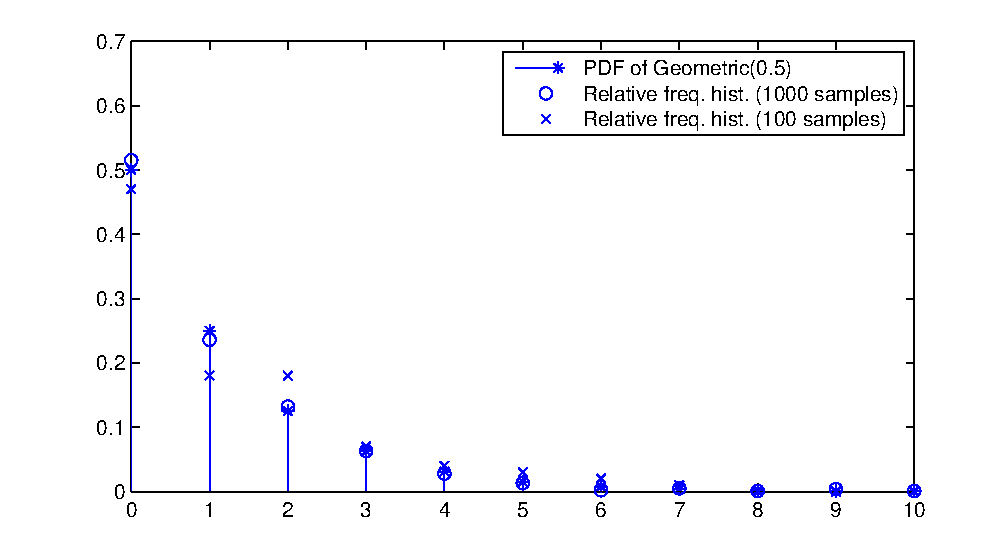
\includegraphics[width=6.50in]{figures/PlotPdfSimHistGeomthetaHalf}}
\end{figure}

\begin{labwork}[Compare PDF to the relative frequency histogram of simulated $\geometric(\theta)$ RV]\label{LW:RelFreqHistForGeomSims}
It is a good idea to make a relative frequency histogram of a simulation algorithm and compare that to the PDF of the discrete RV we are simulating from.  We use the following script to create \hyperref[F:PlotPdfSimHistGeomthetaHalf]{Figure \ref*{F:PlotPdfSimHistGeomthetaHalf}}:
\VrbMf[label=PlotPdfSimGeometric.m]{scripts/PlotPdfSimGeometric.m}
\end{labwork}

The RV $Y$ in \hyperref[T:T3XRVs]{Table \ref*{T:T3XRVs}} may be generalized to an experiment $\E{E}_{\theta}^{n}$ with $n$ coin tosses.  
%}% end remove
Let $X_i$ be the Indicator function of the event `Heads on the $i$-th toss' as before.  Then $Y$ defined by,
 \[
 Y := \sum_{i=1}^n X_i := X_1 + X_2 + \cdots + X_n  \ ,
 \]
is the number of `Heads' in $n$ tosses.  
%\remove{
Akin to the second row of \hyperref[T:T3XRVs]{Table \ref*{T:T3XRVs}}, for the `Toss $n$ times' experiment $\E{E}_{\theta}^{n}$ the
%} 
RV $Y$ as defined above will take values in $\{0,1,2,\ldots,n\}$ and is therefore a discrete RV.  This is called the Binomial RV as defined next.  
%\remove{
But, first we remind ourselves of some elementary definitions involving arrangements of objects from a collection (recall \hyperref[S:PermsFactsCombs]{Section~\ref*{S:PermsFactsCombs}}).
%}%end remove

\begin{model}[$\binomial(n,\theta)$ RV]
Let the RV $X=\sum_{i=1}^n X_i$ be the sum of $n$ independent and identically distributed $\bernoulli(\theta)$ RVs, i.e.:
\[
X=\sum_{i=1}^n X_i, \qquad X_1,X_2,\ldots,X_n \overset{\IID}{\sim} \bernoulli(\theta) \ .
\]
Given two parameters $n$ and $\theta$, the PMF of the $\binomial(n,\theta)$ RV $X$ is:
\begin{equation}
 f(x; n,\theta) =
 \begin{cases}
 \displaystyle\binom{n}{x} \theta^x (1-\theta)^{n-x} & \text{if $x \in \{0,1,2,3,\ldots,n\}$} \ ,\\
 0 & \text{otherwise}
 \end{cases}
 \end{equation}
where, $\binom{n}{x}$ is:
\[
\binom{n}{x} = \frac{n(n-1)(n-2)\ldots(n-x+1)}{x(x-1)(x-2)\cdots (2)(1)} =  \frac{n !}{x! (n-x)!} \ .
 \]
$\binom{n}{x}$ is read as ``$n$ choose $x$.''
 \end{model}
 %{\scriptsize
\begin{proof}
Observe that for the $\binomial(n,\theta)$ RV $X$, $\p(X=x) = f(x;n,\theta)$ is the probability that $x$ of the $n$ $\bernoulli(\theta)$ trials result in an outcome of $1$'s.  Next note that if all $n$ $X_i$'s are $0$'s, then $X=0$, and if all $n$ $X_i$'s are $1$'s, then $X=n$.  In general, if some of the $n$ $X_i$'s are $1$'s and the others are $0$, then $X$ can only take values in $\{0,1,2,\ldots,n\}$ and therefore $f(x;n,\theta)=0$ if $x \notin \{0,1,2,\ldots,n\}$.

Now, let us compute $f(x;n,\theta)$ when $x\in\{0,1,2,\ldots,n\}$.  Consider the set of indices $\{1,2,3,\ldots,n\}$ for the $n$ IID $\bernoulli(\theta)$ RVs $\{X_1,X_2,\ldots,X_n\}$.  Now choose $x$ indices from $\{1,2,\ldots,n\}$ to mark those trials in a particular realization of $\{x_1,x_2,\ldots,x_n\}$ with the Bernoulli outcome of $1$.  The probability of each such event is $\theta^x (1-\theta)^{n-x}$ due to the IID assumption.  For each realization $\{x_1,x_2,\ldots,x_n\} \in \{0,1\}^{n} := \{ \text{all binary $(0-1)$ strings of length $n$}\}$, specified by a choice of $x$ trial indices with Bernoulli outcome $1$, the binomial RV $X=\sum_{i=1}^n X_i$ takes the value $x$.  Since there are exactly $\binom{n}{x}$ many ways in which we can choose $x$ trial indices (with outcome $1$) from the set of $n$ trial indices $\{1,2,\ldots,n\}$, we get the desired product for $f(x; n,\theta) = \binom{n}{x} \theta^x (1-\theta)^{n-x}$ when $x \in \{0,1,\ldots,n\}$.
\end{proof}
%}
\paragraph{Mean and variance of $\binomial(n,\theta)$ RV:}
Let $X \sim \binomial(n,\theta)$.  Based on the definition of expectation:
\[
\e(X) = \int x \, dF(x; n,\theta) = \sum_x x f(x;n,\theta) = \sum_{x =0}^n x \binom{n}{x} \theta^x (1-\theta)^{n-x} \ .
\]
However, this is a nontrivial sum to evaluate.  Instead, we may use \eqref{E:EofLinCombofRVs} and \eqref{E:VofLinCombofRVs} by noting that $X = \sum_{i=1}^n X_i$, where the $\{X_1,X_2,\ldots,X_n \} \overset{\IID}{\sim} \bernoulli(\theta)$, $\e(X_i) = \theta$ and $\V(X_i)=\theta(1-\theta)$:
\[
\e(X) = \e(X_1+X_2, \cdots ,X_n) = \e \left( \sum_{i=1}^n X_i \right) = \sum_{i=1}^n \e(X_i) = n \theta \ ,
\]
\[
\V(X) = \V \left( \sum_{i=1}^n X_i \right) = \sum_{i=1}^n \V(X_i) = \sum_{i=1}^n{\theta(1-\theta)} = n\theta(1-\theta) \ .
\]

%\remove{
\begin{labwork}[Binomial coefficient]\label{LW:BinomialPdf}
We may implement the \Matlab function {\tt BinomialCoefficient} to compute:
\[
\binom{n}{x} =  \frac{n !}{x! (n-x)!} = \frac{n(n-1)(n-2)\ldots(n-x+1)}{x(x-1)(x-2)\cdots (2)(1)} = \frac{\prod_{i=(n-x+1)}^n i}{\prod_{i=2}^x} \ ,
\]
with the following M-file:
\VrbMf[label=BinomialCoefficient.m]{scripts/BinomialCoefficient.m}
and call {\tt BinomialCoefficient} in the function {\tt BinomialPdf} to compute the PDF $f(x;n,\theta)$ of the $\binomial(n,\theta)$ RV $X$ as follows:
\VrbMf[label=BinomialPdf.m]{scripts/BinomialPdf.m}
For example, we can compute the desired PDF for an array of samples {\tt x} from $\binomial(8,0.5)$ RV $X$, as follows:
\begin{VrbM}
>> x=0:1:8
x =     0     1     2     3     4     5     6     7     8
>> BinomialPdf(x,8,0.5)
ans =    0.0039    0.0312    0.1094    0.2188    0.2734    0.2188    0.1094    0.0312    0.0039
\end{VrbM}
\end{labwork}

\begin{simulation}[$\binomial(n,\theta)$ as $\sum_{i=1}^n \bernoulli(\theta)$]\label{SIM:BinomialFromBernoulliSum}
Since the $\binomial(n,\theta)$ RV $X$ is the sum of $n$ IID $\bernoulli(\theta)$ RVs we can also simulate from $X$ by first simulating $n$ IID $\bernoulli(\theta)$ RVs and then adding them up as follows:
\begin{VrbM}
>> rand('twister',17678);
>> theta=0.5; % give some desired theta value, say 0.5
>> n=5; % give the parameter n for Binomial(n,theta) RV X, say n=5
>> xis=floor(rand(1,n)+theta) % produce n IID samples from Bernoulli(theta=0.5) RVs X1,X2,...Xn
xis =     1     1     0     0     0
>> x=sum(xis) % sum up the xis to get a sample from Binomial(n=5,theta=0.5) RV X
x =     2
\end{VrbM}
It is straightforward to produce more than one sample from $X$ by exploiting the column-wise summing property of \Matlab's {\tt sum} function when applied to a two-dimensional array:
\begin{VrbM}
>> rand('twister',17);
>> theta=0.25; % give some desired theta value, say 0.25 this time
>> n=3; % give the parameter n for Binomial(n,theta) RV X, say n=3 this time
>> xis10 = floor(rand(n,10)+theta) % produce an n by 10 array of IID samples from Bernoulli(theta=0.25) RVs
xis10 =
     0     0     0     0     1     0     0     0     0     0
     0     1     0     1     1     0     0     0     0     0
     0     0     0     0     0     0     0     1     0     0
>> x=sum(xis10) % sum up the array column-wise to get 10 samples from Binomial(n=3,theta=0.25) RV X
x =     0     1     0     1     2     0     0     1     0     0
\end{VrbM}
\end{simulation}

In \hyperref[SIM:BinomialFromBernoulliSum]{Simulation \ref*{SIM:BinomialFromBernoulliSum}}, the number of IID $\bernoulli(\theta)$ RVs needed to simulate one sample from the $\binomial(n,\theta)$ RV is exactly $n$.  Thus, as $n$ increases, the amount of time needed to simulate from $\binomial(n,\theta)$ is $O(n)$, i.e.~linear in $n$.  We can simulate more efficiently by exploiting a simple relationship between the $\geometric(\theta)$ RV and the $\binomial(n,\theta)$ RV.

\begin{figure}[htpb]
\caption{PDF of $X \sim \binomial(n=10,\theta=0.5)$ and the relative frequency histogram based on $100,000$ samples from $X$.\label{F:PlotPdfSim10000HistBinomByGeomsn10thetaHalf}}
\centering   \makebox{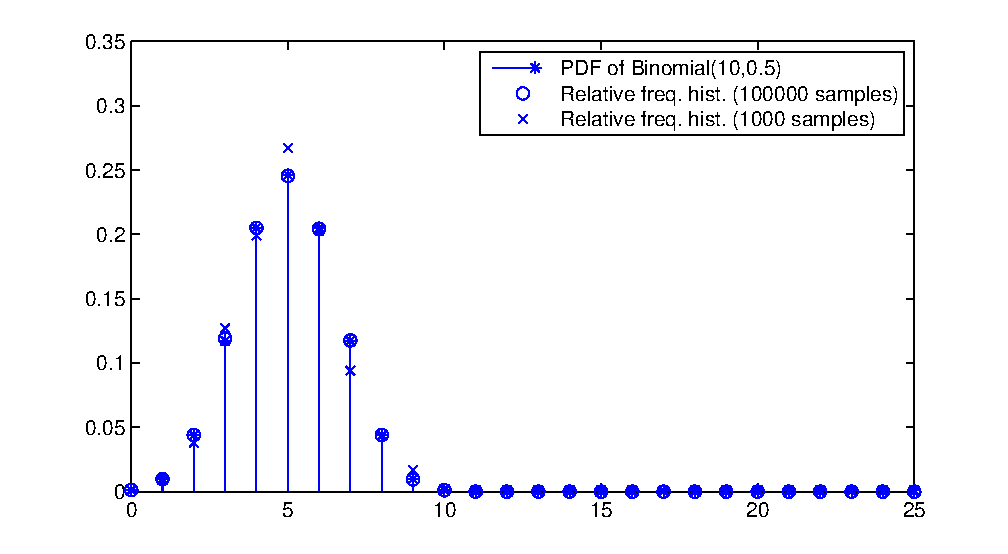
\includegraphics[width=6.50in]{figures/PlotPdfSim10000HistBinomByGeomsn10thetaHalf}}
\end{figure}

The $\binomial(n,\theta)$ RV $X$ is related to the IID $\geometric(\theta)$ RV $Y_1,Y_2,\ldots$: $X$ is the number of successful $\bernoulli(\theta)$ outcomes (outcome is $1$) that occur in a total of $n$ $\bernoulli(\theta)$ trials, with the number of trials between consecutive successes distributed according to IID $\geometric(\theta)$ RV.
\begin{simulation}[$\binomial(\theta)$ from IID $\geometric(\theta)$ RVs]\label{SIM:BinomialFromGeoms}
By this principle, we can simulate from the $\binomial(\theta)$ $X$ by {\sf Step 1}: generating IID $\geometric(\theta)$ RVs $Y_1,Y_2,\ldots$, {\sf Step 2}: stopping as soon as $\sum_{i=1}^k (Y_i+1) > n$ and {\sf Step 3:} setting $x \gets k-1$.

We implement the above algorithm via the following M-file:
\VrbMf[label=Sim1BinomByGeoms.m]{scripts/Sim1BinomByGeoms.m}
Here is a call to simulate $12$ samples from $\binomial(n=10,\theta=0.5)$ RV:
\begin{VrbM}
>> theta=0.5; % declare theta
>> n=10; % say n=10
>> SampleSize=12;% say you want to simulate 12 samples
>> rand('twister',10001) % seed the fundamental sampler
>> Samples=arrayfun(@(T)Sim1BinomByGeoms(n,T),theta*ones(1,SampleSize))
Samples =     7     5     8     8     4     1     4     8     2     4     6     5
\end{VrbM}
\hyperref[F:PlotPdfSim10000HistBinomByGeomsn10thetaHalf]{Figure \ref*{F:PlotPdfSim10000HistBinomByGeomsn10thetaHalf}} depicts a comparison of the PDF of $\binomial(n=10,\theta=0.5)$ RV and a relative frequency histogram based on $100,000$ simulations from it.
\end{simulation}
%}% end remove

In several situations it becomes cumbersome to model the events using the $\binomial(n,\theta)$ RV, especially when when the parameter $\theta \propto 1/n$ and the events become rare.  However, for some real parameter $\lambda>0$, the $\binomial(n,\lambda/n)$ RV with probability of the number of successes in $n$ trials, with per-trial success probability $\lambda/n$, approaches the Poisson distribution with expectation $\lambda$, as $n$ approaches $\infty$ (actually, it converges in distribution as defined later).  The $\poisson(\lambda)$ RV is much simpler to work with than the combinatorially laden $\binomial(n,\theta=\lambda/n)$ RV.  We sketch the details of this next.

%{\scriptsize
Let $X \sim \binomial(n,\theta=\lambda/n)$, then for any $x \in \{0,1,2,3,\ldots,n\}$,
\begin{eqnarray}
\p(X=x)
&=&
\binom{n}{x} \left( \frac{\lambda}{n} \right)^x \left( 1- \frac{\lambda}{n} \right)^{n-x} \notag \\
&=& \frac{n(n-1)(n-2)\cdots(n-x+1)}{x(x-1)(x-2)\cdots (2)(1)}
\left( \frac{\lambda^x}{n^x} \right)
\left( 1- \frac{\lambda}{n} \right)^n
\left( 1- \frac{\lambda}{n} \right)^{-x} \notag \\
&=&
\overbrace{\left( \frac{n}{n} \right) \left( \frac{n-1}{n} \right) \left( \frac{n-2}{n} \right) \cdots \left( \frac{n-x+1}{n} \right)}
\overbrace{\left( \frac{\lambda^x}{x!} \right)}
\underbrace{\left( 1- \frac{\lambda}{n} \right)^n}
\underbrace{\left( 1- \frac{\lambda}{n} \right)^{-x}}  \notag \\
\end{eqnarray}

As $n \to \infty$, the expression below the first overbrace $\to 1$, while that below the second overbrace, being independent of $n$ remains the same.  By the elementary examples of limits
%\remove{
\ref*{EX:LimitExpofLambda} and \ref*{EX:Limit1MinusLambdaOverNToMinusK}%}
, as $n \to \infty$, the expression over the first underbrace approaches $e^{-\lambda}$ while that over the second underbrace approaches $1$.  Finally, we get the desired limit:

\[
\lim_{n \to \infty} \p(X=x)
= \frac{ e^{-\lambda} \lambda^x}{x!}  \ .
\]
%}
\begin{model}[$\poisson(\lambda)$ RV]\label{M:Poisson}
Given a real parameter $\lambda>0$, the discrete RV $X$ is said to be $\poisson(\lambda)$ distributed if $X$ has PDF:
\begin{equation}\label{E:Poissonpdf}
f(x;\lambda) =
\begin{cases}
 \frac{ e^{-\lambda} \lambda^x}{x!} & \text{if $x \in \Zz_+ := \{0,1,2,\ldots\}$} \ , \\
0 & \text{otherwise} \ .
\end{cases}
\end{equation}

Note that the PDF integrates to $1$:
\[
\sum_{x=0}^{\infty} f(x;\lambda)
= \sum_{x=0}^{\infty}  \frac{ e^{-\lambda} \lambda^x}{x!}
=  e^{-\lambda} \sum_{x=0}^{\infty}  \frac{\lambda^x}{x!}
=  e^{-\lambda} e^{\lambda}
= 1 \ ,
\]
where we exploit the Taylor series of $e^{\lambda}$ to obtain the second-last equality above.
\end{model}

\paragraph{Mean and variance of $\poisson(\lambda)$ RV:}
Let $X \sim \poisson(\lambda)$.  Then:
\[
\e(X) = \sum_{x=0}^{\infty} x f(x;\lambda)
= \sum_{x =0}^{\infty} x \frac{ e^{-\lambda} \lambda^x}{x!}
= e^{-\lambda} \sum_{x =0}^{\infty} x \frac{  \lambda^x}{x!}
= e^{-\lambda} \sum_{x -1 =0}^{\infty} \frac{ \lambda \lambda^{x-1}}{(x-1)!}
= e^{-\lambda} \lambda e^{\lambda}
= \lambda
\ .
\]
Similarly,
\[
\V(X) = \e(X^2)-(\e(X))^2 = \lambda + \lambda^2 - \lambda^2 = \lambda \ .
\]
since
\begin{align*}
\e(X^2)& = \sum_{x=0}^{\infty} x^2 \frac{e^{-\lambda} \lambda^x}{x!} = \lambda \, e^{-\lambda} \sum_{x=1}^{\infty} \frac{x \, \lambda^{x-1}}{(x-1)!}
= \lambda \, e^{-\lambda} \left( 1 + \frac{2 \lambda}{1} + \frac{3 \lambda^2}{2!} + \frac{4 \lambda^3}{3!} + ... \right)\\
&= \lambda \, e^{-\lambda} \left( \left( 1 + \frac{\lambda}{1} + \frac{\lambda^2}{2!} + \frac{\lambda^3}{3!} + ... \right) + \left[ \frac{\lambda}{1} + \frac{2 \lambda^2}{2!} + \frac{3 \lambda^3}{3!} + ... \right] \right)\\
&= \lambda \, e^{-\lambda} \left( \left( e^{\lambda} \right) + \lambda \left( 1 + \frac{2 \lambda}{2!} + \frac{3 \lambda^2}{3!} + ... \right) \right)
= \lambda \, e^{-\lambda} \left( e^{\lambda} + \lambda \left( 1 + \lambda + \frac{\lambda^2}{2!} + ... \right) \right)\\
&= \lambda \, e^{-\lambda} \left( e^{\lambda} + \lambda \left( e^{\lambda} \right) \right)
= \lambda \, e^{-\lambda} \left( e^{\lambda} + \lambda\, e^{\lambda}\right) = \lambda (1 + \lambda) = \lambda + \lambda^2
\end{align*}

Note that $\poisson(\lambda)$ distribution is one whose mean and variance are the same, namely $\lambda$.

%\remove{
\begin{figure}[htpb]
\caption{PDF of $X \sim \poisson(\lambda=10)$ and the relative frequency histogram based on 1000 samples from $X$.\label{F:PlotPdfSim1000HistPoiss10}}
\centering   \makebox{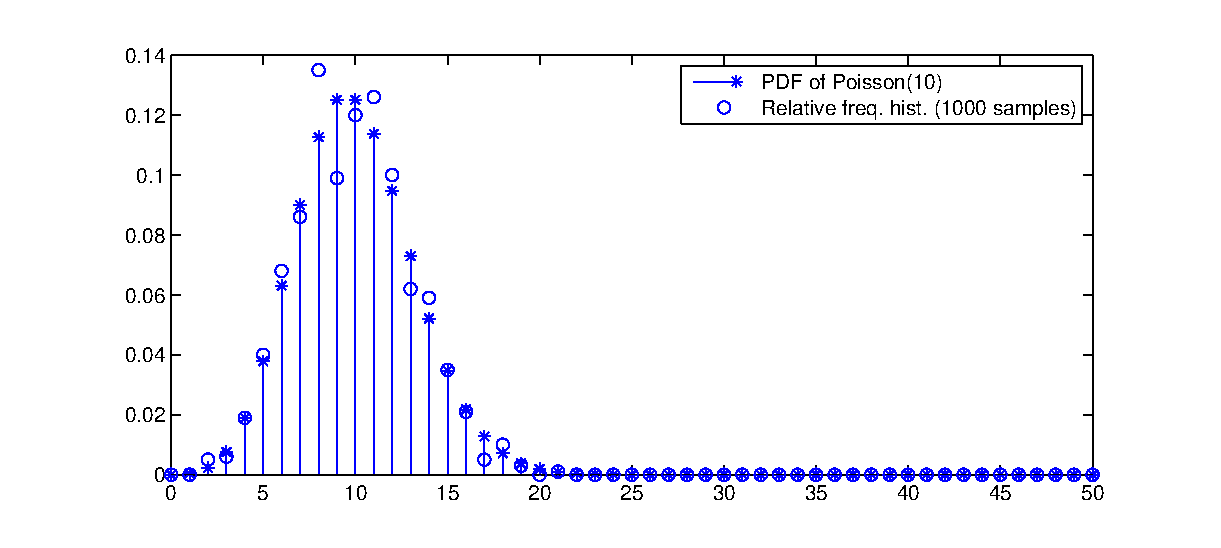
\includegraphics[width=6.50in]{figures/PlotPdfSim1000HistPoiss10}}
\end{figure}
%}%end remove

The $\poisson(\lambda)$ RV $X$ is also related to the IID $\exponential(\lambda)$ RV $Y_1,Y_2,\ldots$: $X$ is the number of occurrences, per unit time, of an instantaneous event whose inter-occurrence time is the IID $\exponential(\lambda)$ RV.  For example, the number of buses arriving at our bus-stop in the next minute, with exponentially distributed inter-arrival times, has a Poisson distribution.
%\remove{
\begin{simulation}[$\poisson(\lambda)$ from IID $\exponential(\lambda)$ RVs]\label{SIM:Poisson}
By this principle, we can simulate from the $\poisson(\lambda)$ $X$ by {\sf Step 1}: generating IID $\exponential(\lambda)$ RVs $Y_1,Y_2,\ldots$, {\sf Step 2}: stopping as soon as $\sum_{i=1}^k Y_i \geq 1$ and {\sf Step 3:} setting $x \gets k-1$.

We implement the above algorithm via the following M-file:
\VrbMf[label=Sim1Poisson.m]{scripts/Sim1Poisson.m}
Here is a call to simulate 10 samples from $\poisson(\lambda=10.0)$ and $\poisson(\lambda=0.1)$ RVs:
\begin{VrbM}
>> arrayfun(@(lambda)Sim1Poisson(lambda),10.0*ones(1,10)) % lambda=10.0
ans =    14     7    10    13    11     3     6     5     8     5
>> arrayfun(@(lambda)Sim1Poisson(lambda),0.1*ones(1,10)) % lambda=0.1
ans =     2     0     0     0     0     0     0     0     0     0
\end{VrbM}
\hyperref[F:PlotPdfSim1000HistPoiss10]{Figure \ref*{F:PlotPdfSim1000HistPoiss10}} depicts a comparison of the PDF of $\poisson(\lambda=10)$ RV and a relative frequency histogram based on 1000 simulations from it.
\end{simulation}

Simulating from a $\poisson(\lambda)$ RV is also a special case of simulating from the following more general RV.
\begin{model}[$GD(\theta_0,\theta_1,\ldots)$]
We say $X$ is a $\generaldiscrete(\theta_0,\theta_1,\ldots)$ or $\GD(\theta_0,\theta_1,\ldots)$ RV over the countable discrete state space $\Zz_+ := \{0,1,2,\ldots\}$ with parameters $(\theta_0,\theta_1,\ldots)$ if the PMF of $X$ is defined as follows:
\[
f(X=x; \theta_0,\theta_1,\ldots) =
\begin{cases}
0, & if \quad x \notin  \{0,1,2,\ldots\} \\
 \theta_0, & if \quad x=0 \\
 \theta_1, & if \quad x=1 \\
\vdots & \\
\end{cases}
\]
\hyperref[A:InvSGenDisc]{Algorithm \ref*{A:InvSGenDisc}} allows us to simulate from any member of the class of non-negative discrete RVs as specified by the probabilities $(\theta_0,\theta_1,\ldots)$.  When an RV $X$ takes  values in another countable set $\Xz \neq \Zz_+$, then we can still use the above algorithm provided we have a one-to-one and onto mapping $D$ from $\Zz_+$ to $\Xz$ that allows us to think of $\{0,1,2,\ldots\}$ as indices of an array $D$.
\end{model}

\begin{algorithm}
\caption{Inversion Sampler for $GD(\theta_0,\theta_1,\ldots)$ RV $X$}
\label{A:InvSGenDisc}
\begin{algorithmic}[1]
\STATE {
{\it input:}
\begin{enumerate}
\item $\theta_0$ and $\{ C(i)  = \theta_{i}/\theta_{i-1} \}$ for any $i \in \{1,2,3,\ldots\}$.
\item $u \sim \uniform(0,1)$
\end{enumerate}
}
\STATE {\it output:} a sample from $X$
\STATE {\it initialise:} $p \gets \theta_0$, $q \gets \theta_0$, $i \gets 0$
\WHILE{$u > q$}
\STATE $i \gets i+1$, $p \gets p \ C(i)$, $q \gets q+p$
\ENDWHILE
\STATE {\it return:} $x = i$
\end{algorithmic}
\end{algorithm}

%\begin{classwork}
%What is the algorithm's efficiency when applied to the $\demoivre(\theta_1,\theta_2,\ldots,\theta_k)$ ?
%Worst-case and average-case efficiency ?
%\vspace{5cm}
%\end{classwork}


\begin{simulation}[$\binomial(n,\theta)$]
To simulate from a $\binomial(n,\theta)$ RV $X$, we can use \hyperref[A:InvSGenDisc]{Algorithm \ref*{A:InvSGenDisc}} with:
\[
\theta_0=(1-\theta)^n, \qquad C(x+1)=\frac{\theta(n-x)}{(1-\theta)(x+1)}, \qquad \text{Mean Efficiency: $O(1+n\theta)$} \ .
\]
\end{simulation}
Similarly, with the appropriate $\theta_0$ and $C(x+1)$, we can also simulate from the $\geometric(\theta)$ and $\poisson(\lambda)$ RVs.

\begin{labwork}This is a challenging exercise for the student who is finding the other Labworks too easy. So those who are novice to \Matlab may skip this Labwork.
\begin{enumerate}
\item Implement \hyperref[A:InvSGenDisc]{Algorithm \ref*{A:InvSGenDisc}} via a function named {\tt MyGenDiscInvSampler} in {\tt MATLAB}.  Hand in the {\tt M-file} named {\tt MyGenDiscInvSampler.m} giving detailed comments explaining your understanding of each step of the code.  [Hint: $C(i)$ should be implemented as a function (use function handles via {\tt @}) that can be passed as a parameter to the function {\tt MyGenDiscInvSampler}].
\item Show that your code works for drawing samples from a $\binomial(n,p)$ RV by doing the following:
\begin{enumerate}
\item Seed the fundamental sampler by your Student ID (if your ID is {\tt 11424620} then type {\tt rand('twister', 11424620);})
\item Draw 100 samples from the $\binomial(n=20,p=0.5)$ RV and report the results in an $2 \times 2$ table with column headings {\tt x} and {No. of observations}.  [Hint: the inputs $\theta_0$ and $C(i)$ for the $\binomial(n,p)$ RV is given above].
\end{enumerate}
\item Show that your code works for drawing samples from a $\geometric(p)$ RV by doing the following:
\begin{enumerate}
\item Seed the fundamental sampler by your Student ID.
\item Set the variable {\tt Mytheta=rand}.
\item Draw 100 samples from the $\geometric({\tt Mytheta})$ RV and report the sample mean.  [Note: the inputs $\theta_0$ and $C(i)$ for the $\geometric(\theta)$ RV should be derived and the workings shown].
\end{enumerate}
\end{enumerate}
\end{labwork}

To make concrete sense of the $\binomial(n,\theta)$ and other more sophisticated concepts in the sequel, let us take a historical detour into some origins of statistical thinking in 19th century England.

\section{Sir Francis Galton's Quincunx}\label{S:Quincunx}
This section is introduced to provide some forms for a kinesthetic (hands-on) and visual understanding of some elementary statistical distributions and laws.  The following words are from Sir Francis Galton, F.R.S., {\em Natural Inheritance}, pp.~62-65, Macmillan, 1889.  In here you will already find the kernels behind the construction of $\binomial(\theta)$ RV as sum of IID $\bernoulli(\theta)$ RVs, Weak Law of Large Numbers, Central Limit Theorem, and more.  We will mathematically present these concepts in the sequel as a way of giving precise meanings to Galton's observations with his Quincunx.
{\it ``{\em The Charms of Statistics}.--It is difficult to understand why statisticians commonly limit their inquiries to Averages, and do not revel in more comprehensive views.  Their souls seem as dull to the charm of variety as that of the native of one of our flat English counties, whose retrospect of Switzerland was that, it its mountains could be thrown into its lakes, two nuances would be got rid of at once.  An Average is but a solitary fact, whereas if a single other fact be added to it, an entire Normal Scheme, which nearly corresponds to the observed one, starts potentially into existence.

Some people hate the very name of statistics, but I find them full of beauty and interest.  Whenever they are not brutalised, but delicately handled by the higher methods, and are warily interpreted, their power of dealing with complicated phenomenon is extraordinary.  They are the only tools by which an opening can be cut through the formidable thicket of difficulties that bars the path of those who pursue the Science of man.}

\begin{figure}[htpb]
\caption{Figures from Sir Francis Galton, F.R.S., {\em Natural Inheritance}, , Macmillan, 1889.\label{F:GaltonFigure78923}}
\mbox{\subfigure[FIG.~7, FIG.~8, and FIG.~ 9 (p.~63)]{\hspace{-0.15cm} 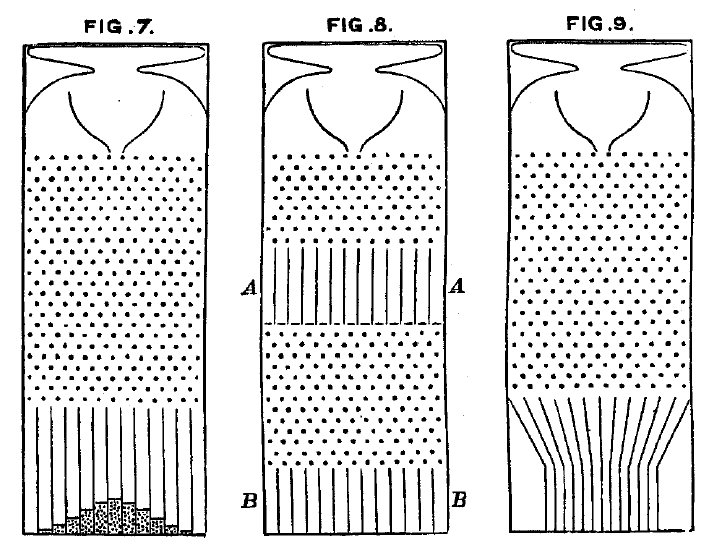
\includegraphics[width=3.250in,clip=,angle=0]{figures/GaltonsFigs789}} \hspace{-0.5cm} \subfigure[FIG.~2 and FIG.~3 (p.~38)]{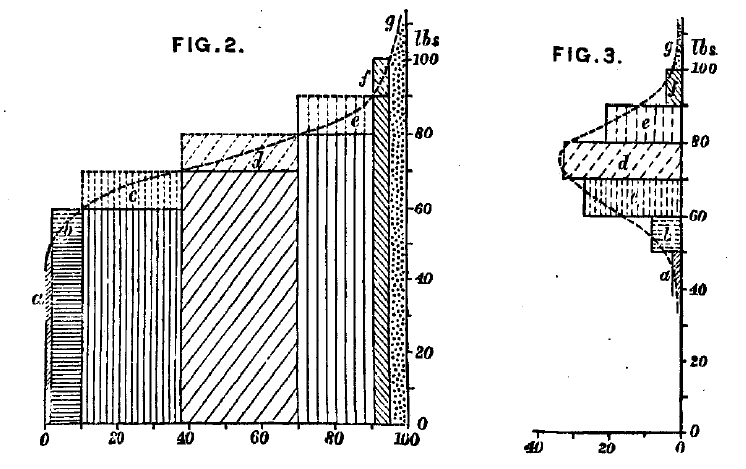
\includegraphics[width=3.40in,clip=,angle=0]{figures/GaltonsFigs23}} }
\end{figure}

{\it {\em Mechanical Illustration of the Cause of the Curve of Frequency}.--The Curve of Frequency, and that of Distribution, are convertible : therefore if the genesis of either of them can be made clear, that of the other also becomes intelligible.  I shall now illustrate the origin of the Curve of Frequency, by means of an apparatus shown in Fig.~7, that mimics in a very pretty way the conditions
on which Deviation depends.  It is a frame glazed in front, leaving a depth of about a quarter of an inch behind the glass.  Strips are placed in the upper part to act as a funnel.  Below the outlet of the funnel stand a succession of rows of pins stuck squarely into the backboard, and below these again are a series of vertical compartments.  A charge of small shot is inclosed.  When the frame is held topsy-turvy, all the shot runs to the upper end; then, when it is turned back into its working position, the desired action commences.  Lateral strips, shown in the diagram, have the effect of directing all the shot that had collected at the upper end of the frame to run into the wide moutn of the funnel.  The shot passes through the funnel and issuing from its narrow end, scampers deviously down through the pins in a curious and interesting way; each of them darting a step to the right or left, as the case may be, every time it strikes a pin.  The pins are disposed in a quincunx fashion, so that every descending shot strikes against a pin in each successive row.  The cascade issuing from the funnel broadens as it descends, and, at length, every shot finds itself caught in a compartment immediately after freeing itself from the last row of pins.  The outline of the columns of shot that accumulate in the successive compartments approximates to the Curve of Frequency (Fig.~3, p.~38), and is closely of the same shape however often the experiment is repeated.  The outline of the columns would become more nearly identical with the Normal Curve of Frequency, if the rows of pins were much more numerous, the shot smaller, and the compartments narrower; also if a larger quantity of shot was used.}

{\it The principle on which the action of the apparatus depends is, that a number of small and independent accidents befall each shot in its career.  In rare cases, a long run of luck continues to favour the course of a particular shot towards either outside place, but in the large majority of instances the number of accidents that cause Deviation to the right, balance in a greater or less degree those that cause Deviation to the left.  Therefore most of the shot finds its way into the compartments that are situated near to a perpendicular line drawn from the outlet of the funnel, and the Frequency with which shots stray to different distances to the right or left of that line diminishes in a much faster ratio than those distances increase.  This illustrates and explains the reason why mediocrity is so common.'' }
%}%end remove

\section*{Summary of Random Variables}\label{S:SummaryRVs}
\begin{table}[ht]
\centering
\begin{tabular}{|c|c|c|c|}%|c}
\hline
Model &PDF&Mean&Variance\\ \hline%&{\tt MGF}\\
%$\pointmass(\theta)$&$\BB{1}_{\{\theta\}}(x)$&$\theta$&$0$\\%&$e^{\theta t}$\\
$\bernoulli(\theta)$ &$\theta^x(1-\theta)^{1-x} \BB{1}_{\{0,1\}}(x)$&$\theta$&$\theta(1-\theta)$\\%&$\theta e^t+(1-\theta)$\\
$\binomial(n,\theta)$&$(^n_{\theta})\theta^x(1-\theta)^{n-x} \BB{1}_{\{0,1,\ldots,n\}}(x)$&$n \theta$&$n \theta(1-\theta)$\\%&$(\theta e^t+(1-\theta))^n$\\
$\geometric(\theta)$ &$\theta(1-\theta)^{x} \BB{1}_{\Zz_+}(x)$&$ \frac{1}{\theta}-1$&$\frac{1-\theta}{\theta^2}$\\%&$\frac{\theta e^t}{1-(1-\theta)e^t}(t<-log(1-\theta))$\\
$\poisson(\lambda)$&$\frac{\lambda^xe^{-\lambda}}{x!} \BB{1}_{\Zz_+}(x)$&$\lambda$&$\lambda$\\%&$e^{\lambda(e^t-1)}$\\
$\uniform(\theta_1,\theta_2)$&$\BB{1}_{[\theta_1,\theta_2]}(x)/(\theta_2-\theta_1)$&$\frac{\theta_1+\theta_2}{2}$&$\frac{(\theta_2-\theta_1)^2}{12}$\\%&$\frac{e^{\theta_2 t}-e^{\theta_1 t}}{(\theta_2-\theta_1)t}$\\
$\exponential(\lambda)$&$\lambda e^{-\lambda x}$&$\lambda^{-1}$&$\lambda^{-2}$\\%&$\frac{1}{1-\frac{1}{\lambda} t}(t<\lambda)$\\
$\normal(\mu,\sigma^2)$&$\frac{1}{\sigma\sqrt{2\pi}}e^{(x-\mu)^2/(2\sigma^2)}$&$\mu$&$\sigma^2$\\%&$exp\{ut+\frac{\sigma^2t^2}{2}\}$\\
$\gammA(\alpha,\beta)$&$\frac{\beta^{\alpha}}{\Gamma(\alpha)}{x^{\alpha-1}e^{-\beta x}}$&$\alpha/\beta$&$\alpha/\beta^2$\\%&$(\frac{1}{1-\beta t})^{\alpha}(t<1/\beta)$\\
%$\betA(\alpha,\beta)$ & $\frac{\Gamma(\alpha+\beta)}{\Gamma(\alpha)\Gamma(\beta)}x^{\alpha-1}(1-x)^{\beta-1}$ & $\frac{\alpha}{\alpha+\beta}$ & $\frac{\alpha\beta}{(\alpha+\beta)^2 (\alpha+\beta+1)} $ \\%& $ 1+\Sigma^\infty_{k+1}(\Pi^{k-1}_{r=0}\frac{\alpha+r}{\alpha+\beta+r})\frac{t^k}{k\!}$\\
%$t_v$ & $\frac{\Gamma((v+1)/2)}{\Gamma(v/2)}  \frac{1}{(1+x^2/v)^{(v+1)/2}$ &0 (if $v>1$ ) & $\frac{v}{v-2}$  (if $v>2$) & does not exist \\
% $\chi^2_p$&$\frac{1}{\Gamma(p/2)2^{p/2}}x^{(p-2)-1}e^{-x/2}$&$p$&$2p$\\ \hline%&$(\frac{1}{1-2t})^{p/2}(t<1/2)$\\
\hline
\end{tabular}
\caption{Random Variables with PDF, Mean and Variance}
%\label{tab:}
\end{table}

\newpage
\section*{Exercises}

\begin{ExerciseList}
\Exercise
One number in the following table for the probability function of a random variable $X$ is incorrect.  
Which is it, and what should the correct value be?
$$
\begin{array}{c|ccccc}
x&1&2&3&4&5\\\hline
\p(X=x)&0.07&0.10&1.10&0.32&0.40
\end{array}
$$
\Answer
$\p(X=3)$ does not satisfy the condition that $0\leq \p(A)\leq1$ for any event $A$.  
If $\Omega$ is the sample space, then $\p(\Omega)=1$ and so  the correct probability is 
\[
\p(X=3)\;=\;1-0.07-0.10-0.32-0.40\;=\;0.11 \enspace .
\]

\Exercise
Let $X$ be the number of years before a particular type of machine will need replacement.  
Assume that $X$ has the probability function $f(1)=0.1$, $f(2)=0.2$, $f(3)=0.2$, $f(4)=0.2$, $f(5)=0.3$.
\be
\item Find the distribution
  function, $F$,  for $X$, and graph both $f$ and $F$.

\item  Find the probability that the machine needs to be
  replaced during the first 3 years.

\item  Find the probability that the machine needs no
  replacement during the first 3 years.
\ee
\Answer
\be
\item  Tabulate the values for the probability mass function  as follows: $$
\begin{array}{c|ccccc}
x&1&2&3&4&5\\\hline
\p(X=x)&0.1&0.2&0.2&0.2&0.3
\end{array}
$$so the  distribution function is:
\[F(x)\; = \;\p(X \leq x) \;=\;
\begin{cases}
 0 & \text{ if }  0 \leq   x < 1\\
 0.1 & \text{ if } 1 \leq  x < 2\\
0.3 & \text{ if } 2 \leq x < 3\\
 0.5 & \text{ if } 3 \leq x < 4\\
0.7 & \text{ if }  4 \leq x < 5\\
 1& \text{ if }    x \geq 5
\end{cases}
\]

The graphs of $f(x)$ and $F(x)$ for random variable $X$ are shown below:

%TODO\centering   \makebox{\includegraphics[width=6.5in]{figures/fandFfor5YearMachine.png}}



\item The probability that the machine needs to be replaced during the
  first 3 years is:
$$\p(X \leq  3)\;=\;\p(X=1)+\p(X=2)+\p(X=3)\;=\;0.1+0.2+0.2\;=\;0.5\,.$$
(This answer is easily seen  from the distribution function of $X$.)
\item The probability that the machine needs no replacement during the
first three years is
\[ \p(X >  3)\;=\;\, 1-\p(X \leq  3)\,=\, 0.5 \,.\]
\ee

\Exercise
Of 200 adults, 176 own one TV set, 22 own two TV sets, and 2 own three TV sets.  
A person is chosen at random. What is the probability mass function of $X$,  the number of TV sets owned by that person?
\Answer
Assuming that the probability model is being built from the observed relative frequencies, the probability mass function is:
$$
f(x)\;=\;\begin{cases}\frac{176}{200}&x=1\\\frac{22}{200}&x=2\\\frac{2}{200}&x=3\end{cases}$$

\Exercise
Suppose a discrete random variable $X$ has probability function give by
$$\begin{array}{c|cccccccccccc}
x&3&4&5&6&7&8&9&10&11&12&13\\\hline
 \p(X=x)&0.07&0.01&0.09&0.01&0.16&0.25&0.20&0.03&0.02&0.11&0.05
\end{array}
$$
\be
\item[(a)] Construct a row of cumulative probabilities for this table, that
  is, find the distribution function of $X$.
\item[(b)] Find  the following  probabilities.
\bcols{3}
\be
\item[(i)]$\p(X\leq 5)$
\item[(ii)] $\p(X<12)$
\item[(iii)] $\p(X>9)$
\item[(iv)] $\p(X\geq 9)$
\item[(v)] $\p(4 <  X\leq 9)$
\item[(vi)] $\p(4<X<11)$
\ee
\ecols
\ee

\Answer
\begin{itemize}
\item[(a)]  $$\begin{array}{c|cccccccccccc}
x&3&4&5&6&7&8&9&10&11&12&13\\\hline
F(x) =\p(X\leq x)&0.07&0.08&0.17&0.18&0.34&0.59&0.79&0.82&0.84&0.95&1.00
\end{array}
$$

\medskip
\item[(b)]
\be
\item[(i)]$\p(X\leq 5)= F(5) = 0.17$ \\[3pt]
\item[(ii)]$\p(X<12)=\p(X\leq11) = F(11) =0.84$\\[3pt]
\item[(iii)] $\p(X>9)= 1 - \p(X\leq 9) = 1- F(9) =1-0.79=0.21$ \\[3pt]
\item[(iv)] $\p(X\geq 9)=1-\p(X <  9)=1-\p(X\leq 8)=1-0.59=0.41$ \\[3pt]
\item[(v)] $\p(4 <  X\leq 9)= F(9) - F(4) =0.79-0.08=0.71$ \\[3pt]
\item[(vi)] $\p(4<X<11)=\p(4 <  X\leq 10)= F(10) -F(4) =0.82- 0.08=0.74$ \\[3pt]
\ee
\end{itemize}


\Exercise
A box contains 4 right-handed and 6 left-handed screws.  
Two screws are drawn at random without replacement. Let $X$ be the number of left-handed screws drawn.  
Find the probability mass function for $X$, and then calculate  the following probabilities:
\be
\item $\p(X\leq 1)$
\item $\p(X\geq 1)$
\item $\p(X>1)$
\ee
\Answer
Since  we are sampling without replacement,
\begin{eqnarray*}
\p(X=0) &=& \frac{4}{10}\cdot\frac{3}{9} = \frac{2}{15}\quad (\text{one way of drawing two right screws}), \\
\p(X=1) &=& \frac{6}{10}\cdot\frac{4}{9}+\frac{4}{10}\cdot\frac{6}{9} = \frac{8}{15}\quad(\text{two ways of drawing one left and one  right screw}),\\
\p(X=2) &=& \frac{6}{10}\cdot\frac{5}{9} = \frac{1}{3}\quad(\text{one way of drawing two left screws}).
\end{eqnarray*}
So the probability mass function of $X$ is:
\[f(x)\;=\;\p(X=x)\;=\;
\begin{cases}
\frac{2}{15}  & \text{if } x=0\\[3pt]
\frac{8}{15} & \text{if } x=1\\[3pt]
\frac{1}{3}  & \text{if } x=2
\end{cases}\]

The required probabilities are:
\be
\item
$$\p(X\leq1)\;=\;\p(X=0)+\p(X=1)\;=\;\frac{2}{15}+\frac{8}{15}\;=\;\frac{2}{3}$$
\item
$$\p(X\geq 1)\;=\;\p(X=1)+\p(X=2)\;=\;\frac{8}{15}+\frac{1}{3}\;=\;\frac{13}{15}$$
\item
$$\p(X>1)\;=\;\p(X=2)\;=\;\frac{1}{3}$$
\ee

\Exercise
Suppose that  a random variable $X$ has geometric  probability mass function,
  \[f(x)\;=\;\frac{k}{2^x}\quad (x=0,1,2,\dots)\,.\]
\be
\item Find the value of  $k$.
\item  What is  $\p(X\geq 4)$?
\ee
\Answer
\be
\item
Since $f$ is a probability mass function,  $$\sum_{x=0}^\infty\frac{k}{2^x}\;=\;1\,, 
\qquad \text{that is,}\qquad k\,\sum_{x=0}^\infty\frac{1}{2^x}\;=\;1\ \enspace.$$
Now $\displaystyle \sum_{x=0}^\infty\frac{1}{2^x}$ is a geometric series with common ratio $r= \frac{1}{2}$ and first term $a=1$,
and so has  sum
\[ S\;=\; \frac{a}{1-r} \;=\;\frac{1}{1-\frac{1}{2} } \;=\; 2\]
Therefore, \[  2 k\;=\; 1 \,, \quad \text{that
  is,}\quad k\;=\; \frac{1}{2}\,.\]

\item From (a), the probability mass function of $f$ is
  $$f(x)\;=\;\frac{\frac{1}{2}}{2^{x}}\;=\;\frac{1}{2^{x+1}}\,.\quad
  (x=0,1,2,\dots)$$ Now
\[\p(X\geq 4)\;=\;1-\p(X<4)\;=\;1-\p(X\leq3)\] where
\ba{\p(X\leq3)&=\;\sum^3_{x=0}\frac{1}{2^{x+1}}\\[3pt]
&=\;\frac{1}{2}+\frac{1}{4}+\frac{1}{8}+\frac{1}{16}\\[3pt]
&=\;\frac{8}{16}+\frac{4}{16}+\frac{2}{16}+\frac{1}{16}\\[3pt]
&=\;\frac{15}{16}\enspace.
}
That is,  $\p(X\geq4)\,=\,\displaystyle \frac{1}{16}$.
\ee

\Exercise
Four fair coins are tossed simultaneously.  
If we count the number of heads that appear then we have a  binomial random variable,  $X=$ {\it the number of heads}.
\be
\item Find the probability mass
  function of  $X$.
\item  Compute the probabilities of obtaining no heads, precisely 1
  head, at least 1 head, not more than 3 heads.
\ee
\Answer
Note that  $\theta=\frac{1}{2}$ here.
\be
\item $X$ has probability mass function
\[f(x)\;=\;\begin{cases}
\displaystyle\displaystyle \binom{4}{0}\frac{1}{2}^0\frac{1}{2}^4=\frac{1}{16}&x=0\\[16pt]
\displaystyle\displaystyle\binom{4}{1}\frac{1}{2}^1\frac{1}{2}^3=\frac{4}{16}&x=1\\[16pt]
\displaystyle\displaystyle\binom{4}{2}\frac{1}{2}^2\frac{1}{2}^2=\frac{6}{16}&x=2\\[16pt]
\displaystyle\binom{4}{3}\frac{1}{2}^3\frac{1}{2}^1=\frac{4}{16}&x=3\\[16pt]
\displaystyle\binom{4}{4}\frac{1}{2}^4\frac{1}{2}^0=\frac{1}{16}&x=4
\displaystyle\end{cases}
\]

\item The required probabilities are:

$\displaystyle \p(X=0)=f(0)=\frac{1}{16}$\\[3pt]
$\displaystyle \p(X=1)=f(1)=\frac{4}{16}$\\[3pt]
$\displaystyle \p(X\geq1)=1-\p(X=0)=1-f(0)=\frac{15}{16}$\\[3pt]
$\displaystyle \p(X\leq3)=f(0)+f(1)+f(2)+f(3)=\frac{15}{16}$
\ee

\Exercise
The distribution of blood types in a certain  population is as follows:
$$
\begin{array}{c|cccc}
\text{Blood type}&\text{Type } O&\text{Type } A&\text{Type } B& \text{Type }AB\\\hline
\text{Proportion}&0.45&0.40&0.10&0.05
\end{array}
$$
A random sample of 15 blood donors is observed from this
population. Find the probabilities of the following events.

\be
\item Only one type $AB$ donor is included.
\item At least three of the donors are type $B$.
\item More than ten of the donors are \emph{either} type $O$ \emph{or} type $A$.
\item Fewer that five of the donors are \emph{not} type $A$.
\ee
\Answer
\be
\item  If the random variable $X$ denotes the number of type $AB$ blood donors
  in the sample of 15, then $X$ has a binomial distribution with $n=15$
  and $\theta=0.05$.  Therefore
\[\p(X=1) \;=\;\binom{15}{1} (0.05)^1  (0.95)^{14}\;=\;0.366 \quad (\text{3 sig. fig.}) \,.\]

\medskip
\item  If the random variable $X$ denotes the number of type $B$  blood donors
  in the sample of 15, then $X$ has a binomial distribution with $n=15$
  and $\theta=0.10$.  Therefore
\ba{\p(X\geq 3) &\;=\;  1\, - \,\p(X=0)\, -\, \p(X=1)\, -\, \p(X=2) \\[3pt]
 &\;=\;  1\; - \; \binom{15}{0} (0.1)^0  (0.9)^{15}\;-\; \binom{15}{1}
 (0.1)^1  (0.9)^{14}\;-\; \binom{15}{2} (0.1)^2  (0.9)^{13}\\[3pt]
&\;=\;  1\,-\, 0.2059 \,-\, 0.3432 \,-\, 0.2669\\[3pt]
&\;=  \;0.184 \quad (\text{to 3 sig. fig.})
}

\medskip
\item If the random variable $X$ denotes the number of type  $O$ or type $A$ blood donors
  in the sample of 15, then $X$ has a binomial distribution with $n=15$
  and $\theta=0.85$.  Therefore
\ba{\p(X > 10 ) &\;=\;  \p(X=11)\, + \, \p(X=12)\, +\,  \p(X=13) \, + \, \p(X=14)\, + \, \p(X=15)  \\[3pt]
 &\;=\;   \binom{15}{11} (0.85)^{11}  (0.15)^{4}\;+\; \binom{15}{12}
 (0.85)^{12}  (0.15)^{3}\\[3pt]
&\;+\; \binom{15}{13} (0.85)^{13}  (0.15)^{2}\;+\; \binom{15}{14} (0.85)^{14}  (0.15)^{1}\;+\; \binom{15}{15} (0.85)^{15}  (0.15)^{0}\\[3pt]
&\;=\;  0.1156 \,+\,0.2184 \,+\,0.2856 \,+\, 0.2312\,+\,0.0874\\[3pt]
&\;=\;0.938 \quad (\text{to 3 sig. fig.})
}

\medskip
\item If the random variable $X$ denotes the number of blood donors that
  are \emph{not} of type $A$ blood donors
  in the sample of 15, then $X$ has a binomial distribution with $n=15$
  and $\theta=0.6$.  Therefore
\ba{\p(X <  5) &\;=\;  \p(X=0)\, +\, \p(X=1)\, + \, \p(X=2)\, + \, \p(X=3)\, + \, \p(X=4) \\[3pt]
 &\;=\;   \binom{15}{0} (0.6)^0  (0.4)^{15}\;+\; \binom{15}{1}
 (0.6)^1  (0.4)^{14}\;+\; \binom{15}{2} (0.6)^2  (0.4)^{13}\\[3pt]
&\;+\; \binom{15}{3} (0.6)^3  (0.4)^{12}\;+\; \binom{15}{4} (0.6)^4  (0.4)^{11}\\[3pt]
&\;=\;  0.0000 \,+\,  0.0000\,+\, 0.0003\,+\, 0.0016\,+\,0.0074\\[3pt]
&\;=\;0.009 \quad (\text{to 3 DP.})
}
\ee



\Exercise
If the probability of hitting a target in a single shot is $10\%$ and 10 shots are fired independently, what is the probability that the target will be hit at least once?
\Answer
This is a Binomial experiment with parameters $\theta=0.1$ and $n=10$, and so 
\[\p(X\geq 1) = 1-\p(X<1) = 1-\p(X=0) \enspace ,\] 
where
\[\p(X=0) = \binom{10}{0}0.1^0 0.9^{10} \approxeq 0.3487 \enspace .\]

 Therefore, the probability that the target will be hit at least once is
 \[1- 0.3487 \approxeq 0.6513 \enspace .\]

\Exercise
Consider the probability density function
$$f(x)\;=\;\begin{cases} k &-4 \leq x\leq4\\0&\textrm{otherwise}\end{cases}\,.$$

\be
\item Find  the value of $k$.
\item Find the distribution function, $F$.
\item   Graph $f$ and  $F$.
\ee
\Answer
\be
\item Since $f(x)$ is a (continuous) probability density function which integrates to one,
$$\int_{-4}^4kdx\;=\;1\,.$$
That is, 
\ba{k \,x\bigg]^4_{-4}&=\;1\\[3pt]k(4-(-4))&=\;1\\[3pt]8k&=\;1\\[3pt]k&=\;\frac{1}{8}}

\item First note that if $x <  -4$, then  $$F(x)\;=\;\int^x_{-\infty}0\,dv\;=\;0\,.$$
If $-4 \leq x \leq 4$, then
\begin{align*}F(x)&=\;\int^{-4}_{-\infty}0\,dv\;+\;\int^x_{-4} \frac{1}{8}\,dv\\[3pt]
&=\;0\;+\;\left[ \frac{1}{8}\, v \right]^x_{-4}\\[3pt]
&=\;  \frac{1}{8} (x +4)\end{align*}
If $x\geq 4$, then
\begin{align*}F(x)&=\int^{-4}_{-\infty}0\,dv\;+\;\int^{4}_{-4}
  \frac{1}{8} \,dv\;+\;\int^x_{4} 0 \,dv\\[3pt]
&=0\;+\;\left[\frac{1}{8} v \right]^4_{-4}\;+\;0\\[3pt]
&=\; 1\end{align*}
Hence  $$F(x)\;=\;\begin{cases}0&x <  -4\\ \frac{1}{8} (x+4) &-4 \leq
  x\leq 4\\1&x\geq 4\end{cases}$$

\item  The graphs of $f(x)$ and $F(x)$ for  random variable $X$ are as follows:
%TODO\centering   \makebox{\includegraphics[width=6.5in]{figures/fandFforConstantDensity.png}}

\ee

\Exercise
Assume that a new light bulb will burn out at time $t$ hours according to the probability density function given by 
$$
f(t)\;=\;
\begin{cases}
\lambda e^{-\lambda t} & \text{ if } t >0 \enspace,\\
0 & \text{ otherwise} \enspace .
\end{cases}
$$
In this context, $\lambda$ is often called the failure rate of the bulb.

\be
\item[(a)]Assume that $\lambda=0.01$, and find the probability that the
  bulb will not burn out before $\tau$ hours. This $\tau$-specific probability is often
  called the reliability of the bulb.

Hint: Use the distribution function for an $\exponential(\lambda)$ random variable (recall, $F(\tau;\lambda)=\int_{-\infty}^{\tau} f(t) dt$)!

\item[(b)]For what  value of $\tau$ is the reliability of the bulb exactly $\frac{1}{2}$?
\ee
\Answer
\be
\item Since the distribution function is $F(t; \lambda) \,=\,
  1 - \exp( - \lambda t)$,
 \[\p(t>\tau)\;=\;1-\p(t<\tau)\;=\; 1 - F(\tau;\lambda=0.01) \;=\;1-(1-e^{-0.01\tau})\;=\;e^{-0.01\tau}\,.\]

\item Set  \[\p(t>\tau)\;=\;e^{-0.01\tau}\;=\;\frac{1}{2}\]
and solve for $\tau$ to get  then $\tau\,=\,-100\times \log(0.5)\,=\,69.3\quad (\text{3 sig. fig.})$\,.
\ee

\Exercise
Feller discusses the probability and statistics of flying bomb hits in an area of southern London during II world war.  
The area in question was partitioned into $24 \times 24 = 576$ small squares.  
The total number of hits was $537$.  
There were $229$ squares with $0$ hits, $211$ with $1$ hit, $93$ with $2$ hits, $35$ with $3$ hits, $7$ with $4$ hits and $1$ with $5$ or more hits.  
Assuming the hits were purely random, use the Poisson approximation to find the probability that a particular square would have exactly $k$ hits.  Compute the expected number of squares that would have $0$, $1$, $2$, $3$, $4$, and $5$ or more hits and compare this with the observed results (Snell 9.2.14).  
\Answer
We are given that $537$ flying bombs hit an area $A$ of south London made up of $24 \times 24=576$ small equal-sized areas, say $A_1,A_2,\ldots,A_{576}$.  
Assuming the hits were purely random over $A$ the probability that a particular bomb will hit a given small area, say $A_i$, is $\frac{1}{576}$.  
Let $X$ denote the number of hits that a small area $A_i$ receives in this German raid.  
Since $537$ bombs fell over $A$, we can model $X$ as $\binomial(n=537,\theta=\frac{1}{576})$ that is counting the number of `successes' (for German bombers) with probability $\theta$ in a sequence of $n=537$ independent $\bernoulli(\theta)$ trials.  
Finally, we can approximate this $\binomial(n=537,\theta=\frac{1}{576})$ random variable by $\poisson(\lambda)$ random variable with $\lambda=n\theta=\frac{537}{576} \approxeq 0.933$.
Using the probability mass function formula for $\poisson(\lambda=0.933)$ random variable $X$ we can obtain the probabilities and compare them with the relative frequencies from the data as follows:

\begin{center}
{\small
\begin{tabular}{|c|c|c|c|}
\hline
$x$ & observed frequency & observed relative frequency & Prob of $x$ hits\\\hline
$0$ & $229$ & $229/576=0.398$ & $f(0;0.933) = 0.394$\\
$1$ & $211$ & $211/576=0.366$ & $f(1;0.933) = 0.367$\\
$2$ & $93$ & $93/576=0.161$ & $f(2;0.933) = 0.171$\\
$3$ & $35$ & $35/576=0.0608$ & $f(3;0.933) = 0.0532$\\
$4$ & $7$ & $7/576=0.0122$ & $f(4;0.933) = 0.0124$\\
$\geq 5$ & $1$ & $1/576=0.00174$ & $1-\sum_{x=0}^4f(x;0.933) = 0.00275$\\\hline
\end{tabular}
}
\end{center}

%question  (poisson)
\Exercise 
Suppose that a certain type of magnetic tape contains, on the average, 2 defects per 100 meters.  
What is the probability that a roll of tape 300 meters long will contain  no defects?
\Answer
Since 2 defects exist on every 100 meters, we would expect 6 defects on a 300 meter tape.  
If $X$ is the number of defects on a 300 meter tape, then $X$ is Poisson with $\lambda = 6$ and so the probability of zero defects is
$$\p(X=0;6)\;=\;\frac{6^0}{0!}e^{-6}\;=\;0.0025\enspace.$$

%question  (poisson)
\Exercise
In 1910, E.~Rutherford and H.~Geiger showed experimentally that the number of alpha particles emitted per second in a radioactive process is a random variable $X$ having a Poisson distribution. If the average number of particles emitted per second is  0.5, what is the probability of observing two or more particles during any given second?
\Answer
Since $X$ is $\poisson(\lambda)$ random variable with $\lambda=0.5$, $\p(X\geq2)$ 
is the probability of observing two or more particles during any
given second. $$\p(X\geq 2)\;=\;1-\p(X<2)\;=\;1-\p(X=1)-\p(X=0)\enspace,$$
where $\p(X=1)$ and $\p(X=0)$ can be carried out by the Poisson
probability mass function $$\p(X=x)\;=\; f(x)\;=\;\frac{\lambda^x}{x!}e^{-\lambda}\enspace.$$
Now \[\p(X=0)\;=\;\frac{0.5^0}{0!}\,\times \,e^{-0.5} \;=\; 0.6065\] and
\[ \p(X=1)\;=\;\frac{0.5^1}{1!}\,\times \, e^{-0.5}\;=\; 0.3033\] and so
$$\p(X\geq 2)\;=\; 1- 0.9098\;= \;0.0902\enspace.$$

%question  (poisson)
\Exercise 
The number of lacunae (surface pits) on specimens of steel, polished and examined in a metallurgical laboratory, is known to have Poisson distribution.
\be
\item Write down the formula for the probability that a specimen has $x$
  defects, explaining the meanings of the symbols you use.
\item Simplify the formula in the case $x=0$.
\item In a large homogeneous collection of specimens, 10\% have one or more lacunae. Find (approximately) the percentage having exactly two.
\item Why might the Poisson distribution not apply in this situation?
\ee
\Answer
\be
\item The Probability mass function for $\poisson(\lambda)$ random variable $X$ is 
\[\p(X=x)\;=\;f(x;\lambda)\;=\; \frac{e^{-\lambda}\lambda^x}{x!}\]
where $\lambda$ is the mean number of lacunae per specimen and $X$ is
the random variable ``number of lacunae on a specimen''.

\item If $x=0$ then $x!=0!=1$ and $\lambda^x=\lambda^0=1$, and the formula becomes  
$\displaystyle \p(X=0) \,=\, e^{-\lambda}$.

\item Since $\p(X \geq 1) = 0.1$, \[\p( X=0)\;=\; 1 -  \p(X \geq 1)\;=\; 0.9\,.\]

Using (b) and solving for $\lambda$ gives:
\[ e^{-\lambda}\;=\; 0.9 \quad \text{that is,}\quad \lambda \;=\; -\ln(0.9) \;=\; 0.1\;
(\text{approximately}\,.)\]

Hence \[\p( X=2 )\;=\;   \frac{e^{-0.1} (0.1)^2}{2!}  \;=\;0.45\% \;
(\text{approximately}\,.) \]

\item Occurrence of lacunae may not always be independent. For example, a machine malfunction may cause them to be clumped.
\ee

%question 9 (cts )
\Exercise
Find the probability that none of the three bulbs in a traffic signal need to be replaced during the first 1200 hours of operation if the length of time before a single bulb needs to  be replaced is a continuous random variable $X$ with density
$$f(x)\;=\;\begin{cases}6\left(0.25-(x-1.5)^2\right)&1<x<2\\0&\textrm{otherwise}\end{cases}\enspace.$$
Note: $X$ is measured in multiples of 1000 hours.
\Answer
The probability that  \emph{one}  light bulb doesn't need to be replaced in  1200 hours is:
\ba{\p(X>1.2)&\;=\;1-\p(X<1.2)\\[3pt]
&=\;1\;-\;\int^{1.2}_1 6 (0.25-(x-1.5)^2)\,dx\\[3pt]
&=\;1\;-\;\int^{1.2}_1 6(0.25-x^2+3x-2.25)\,dx\\[3pt]
&=\;1\;-\;\int^{1.2}_1 (-6x^2+18x-12)\,dx\\[3pt]
&=\;1\;-\;\left[-2x^3+9x^2-12x\right]^{1.2}_1\\[3pt]
&=\;1-0.1040\\[3pt]
&\;=\;0.8960}
Assuming  that   the three light bulbs function  independently of  each
other, the probability that none of them need to be replaced in the
first 1200 hours is
$$\p(\{X_1>1.2\}\cap\{X_2>1.2\}\cap\{X_3>1.2\}\;=\;0.8960^3\;=\;
0.7193$$
where $X_i$ is the length of time that bulb $i$ lasts.

%question 10 (cts exp )
\Exercise 
Let the random variable $X$ be the time  after which certain ball bearings wear out, with density
$$f(x)\;=\;\begin{cases} ke^{-x}&0\leq x\leq 2\\0&\textrm{otherwise}\end{cases}\enspace.$$
Note: $X$ is measured in  years.
\be
\item Find $k$.
\item Find the probability that a bearing will last at least 1 year.
\ee
\Answer
\be
\item

\ba{\int^2_0 k\,e^{-x}\,dx &=\;1\\[3pt]
\left[ -k\,e^{-x}\right]^2_0&=\;1\\[3pt]
k\,(-e^{-2}+1)&=\;1\\[3pt]
k&=\;\frac{1}{1-e^{-2}} \quad (\approx 1.1565)
}

\item
\ba{\p(X\geq1)&=1\,-\,\p(X<1)\\[3pt]
&=\;1\;-\;\int^1_0 k e^{-x}\,dx\\[3pt]
&=\;1\;+\;k\left(e^{-x}\right]^1_0\\[3pt]
&=\;1\;+\;\frac{e^{-1}-1}{1-e^{-2}}\\[3pt]
&\approx\;0.2689}

\ee

\Exercise
{**}Starting from the definition of the variance of a random variable (Definition~\ref{D:VarianceofX}) show that
\[\V(X) = \e(X^2) - \left(\e(X)\right)^2 \enspace .\]

\Exercise
{**}Let $X$ be a discrete random variable with PMF given by
\[
f(x) = 
\begin{cases}
\frac{x}{10} & \text{ if } x \in \{1,2,3,4\} ,\\
0 & \text{ otherwise.}
\end{cases}
\]
\begin{itemize}
\item[(a)] Find:
\begin{itemize}
\item[(i)] $\p(X=0)$
\item[(ii)] $\p(2.5 < X < 5)$
\item[(iii)] $\e(X)$
\item[(iv)] $\V(X)$
\end{itemize}
\item[(b)] Write down the DF (or CDF) of $X$.
\item[(c)] Plot the PMF and CDF of $X$.
\end{itemize}

\Exercise


\end{ExerciseList}

\newpage

We need a new notion for the variance of two RVs.
\begin{definition}[Covariance]
Suppose $X_1$ and $X_2$ are random variables, such that $\e(X_1^2) < \infty$ and $\e(X_2)^2 < \infty$.  Then, $\e(|X_1 X_2|) < \infty$ and $\e(|(X_1-\e(X_1))(X_2-\e(X_2))|) < \infty$.  We therefore define the covariance $\cv(X_1,X_2)$ of $X_1$ and $X_2$ as:
\[
\cv(X_1,X_2) := \e \left((X_1-\e(X_1))(X_2-\e(X_2))\right) = \e(X_1 X_2) - \e(X_1) \e(X_2)
\]
\end{definition}

Let us consider the natural two-dimensional analogue of the $\bernoulli(\theta)$ RV in the real plane $\Rz^2 := (-\infty,\infty)^2 := (-\infty,\infty) \times (-\infty,\infty)$.  A natural possibility is to use the {\bf ortho-normal basis vectors} in $\Rz^2$:
$$ \boxed{
e_1 := (1,0), \qquad e_2 := (0,1)
} \ .$$
Recall that vector addition and subtraction are done component-wise, i.e.~$(x_1,x_2) \pm (y_1,y_2) = (x_1\pm y_1,x_2 \pm y_2)$.

\begin{classwork}[Geometry of Vector Addition]
Recall elementary vector addition in the plane.  What is $(1,0)+(1,0)$, $(1,0)+(0,1)$, $(0,1)+(0,1)$?  What is the relationship between $(1,0)$, $(0,1)$ and $(1,1)$ geometrically? How does the diagonal of the parallelogram relate the its two sides in the geometry of addition in the plane?  What is  $(1,0)+(0,1)+(1,0)$?
\end{classwork}

\begin{figure}[htpb]
\caption{Quincunx on the Cartesian plane.  Simulations of $\binomial(n=10,\theta=0.5)$ RV as the x-coordinate of the ordered pair resulting from the culmination of sample trajectories formed by the accumulating sum of $n=10$ IID $\bernoulli(\theta=0.5)$ random vectors over $\{(1,0),(0,1)\}$ with probabilities $\{\theta,1-\theta\}$, respectively.  The blue lines and black asterisks perpendicular to and above the diagonal line, i.e.~the line connecting $(0,10)$ and $(10,0)$, are the density histogram of the samples and the PDF of our $\binomial(n=10,\theta=0.5)$ RV, respectively.\label{F:BinomQuincunxn10r10r1000}}
\centering
\mbox{\subfigure[Ten samples]{\hspace{-2cm} \includegraphics[width=3.250in]{figures/BinomQuincunxn10r10}} \hspace{-2cm}
	   \subfigure[Thousand samples]{\includegraphics[width=3.250in]{figures/BinomQuincunxn10r1000}} }
\end{figure}

\begin{model}[$\bernoulli(\theta)$ \rv]
Given a parameter $\theta \in [0,1]$, we say that $X := (X_1,X_2)$ is a $\bernoulli(\theta)$ random vector (\rv) if it has only two possible outcomes in the set $\{e_1,e_2\} \subset \Rz^2$, i.e.~$x:=(x_1,x_2) \in \{(1,0),(0,1)\}$.  The PMF of the \rv~$X:= (X_1,X_2)$ with realisation $x:=(x_1,x_2)$ is:
\[
f(x;\theta) := \p(X=x) = \theta \, \BB{1}_{\{e_1\}}(x) + (1-\theta) \, \BB{1}_{\{e_2\}}(x) =
\begin{cases}
\theta & \text{if } \quad x=e_1:=(1,0) \\
1- \theta & \text{if } \quad x=e_2:=(0,1) \\
0 & \text{otherwise}
\end{cases}
\]
\end{model}


\begin{classwork}[Expectation and Variance of $\bernoulli(\theta)$ \rv]
What is the Expectation of $\bernoulli(\theta)$ \rv?
\[
\e_{\theta}(X) = \e_{\theta}((X_1,X_2)) = \sum_{(x_1,x_2) \in \{e_1,e_2\}} (x_1,x_2) f((x_1,x_2);\theta) = (1,0) \theta + (0,1) (1-\theta) = (\theta,1-\theta) \ .
\]

How about the variance ? [Hint: Use the definitions of $\e(X)$ and $\V(X)$ for the \rv~$X$.  $\e(X^2)$ is not a single number and you may need new words such as covariance to deal with terms like $\e(X_1 X_2)$.]
\end{classwork}

%\remove{
We can write the $\binomial(n,\theta)$ RV $Y$ as a $\binomial(n,\theta)$ \rv~$X:=(Y,n-Y)$.  In fact, this is the underlying model and the {\bf bi} in the $\binomial(n,\theta)$ does refer to two in Latin.  In the coin-tossing context this can be thought of keeping track of the number of Heads and Tails out of an IID sequence of $n$ tosses of a coin with probability $\theta$ of observing Heads.  In the Quincunx context, this amounts to keeping track of the number of right and left turns made by the ball as it drops through $n$ levels of pegs where the probability of a right turn at each peg is independently and identically $\theta$.  In other words, the $\binomial(n,\theta)$ \rv~$(Y,n-Y)$ is the sum of $n$ IID $\bernoulli(\theta)$ {\rv}s $X_1:=(X_{1,1},X_{1,2}), X_2:=(X_{2,1},X_{2,2}), \ldots, X_n:=(X_{n,1},X_{n,2})$:
\[
(Y,n-Y) = X_1+X_2+\cdots + X_n = (X_{1,1},X_{1,2}) + (X_{2,1},X_{2,2}) + \cdots + (X_{n,1},X_{n,2})
\]

Go the Biomathematics Research Centre on the 6th floor of Erskine to play with the Quincunx built by Ryan Lawrence in 2007 (See the project by Ashman and Lawrence at  \href{http://www.math.canterbury.ac.nz/~r.sainudiin/courses/STAT218/projects/Stat218StudentProjects2007.pdf}{\url{http://www.math.canterbury.ac.nz/~r.sainudiin/courses/STAT218/projects/Stat218StudentProjects2007.pdf}} % \ref{S:AshmanLawrenceQuincunx} 
for details).  It is important to gain a physical intimacy with the Quincunx to appreciate the following model of it.  We can make a statistical model of Galton's observations earlier regarding the dynamics of lead shots through the Quincunx as the sum of $n$ IID $\bernoulli(0.5)$ \rv{s}, where $n$ is number of pegs that each ball bounces on before making a left or right turn with equal probability.  

\begin{exercise}[Number of paths and the binomial coefficient]
How does the number of paths that lead to a bucket $(x_1,x_2)$ with $x_1+x_2=n$ relate to the binomial coefficient $\binom{n}{x_1} ?$
%\vspace{2cm}
\end{exercise}

\begin{labwork}[Quincunx Sampler Demo -- Sum of $n$ IID $\bernoulli(1/2)$ \rv{s}]\label{LW:QuincunxSampler}
Let us understand the Quincunx construction of the $\binomial(n,1/2)$ \rv $X$ as the sum of $n$ independent and identical $\bernoulli(1/2)$ \rv{s} by calling the interactive visual cognitive tool as follows:
\begin{VrbM}
>> guiMultinomial
\end{VrbM}
The M-file {\tt guiMultinomial.m} will bring a graphical user interface (GUI) as shown in \hyperref[F:guiMultinomialQuincunx]{Figure \ref*{F:guiMultinomialQuincunx}}.  Using the drop-down menu at ``How many levels?'' change the number of levels to $2$ ($n=2$).  Now click the ``Do one'' button as many times as you like and comprehend the simulation process -- the path taken by the ball as it falls through two levels.  Next, from the drop-down menu at ``How many  Replication?'' change it from $10$ to $100$.  You can press ``Do all'' to watch all 100 balls drop into their possible values at level $2$.  Change the number of levels or $n$ in $\binomial(n,1/2)$ \rv to $3$ or $5$ or $10$ and do more simulations until you are comfortable with the construction that the sum of $n$ IID $\bernoulli(1/2)$ \rv{s} is the $\binomial(n,1/2)$ \rv.

When we drop $1000$ balls into the simulated Quincunx the density histogram is much closer to the PDF of $\binomial(n=10,\theta=0.5)$ RV than when we only drop $10$ balls.  See \hyperref[F:BinomQuincunxn10r10r1000]{Figure \ref*{F:BinomQuincunxn10r10r1000}} for a description of the simulations.  Try to replicate such a simulation on your own.
\end{labwork}

\begin{figure}[htpb]
\caption{Visual Cognitive Tool GUI: Quincunx.\label{F:guiMultinomialQuincunx}}
\centering   \makebox{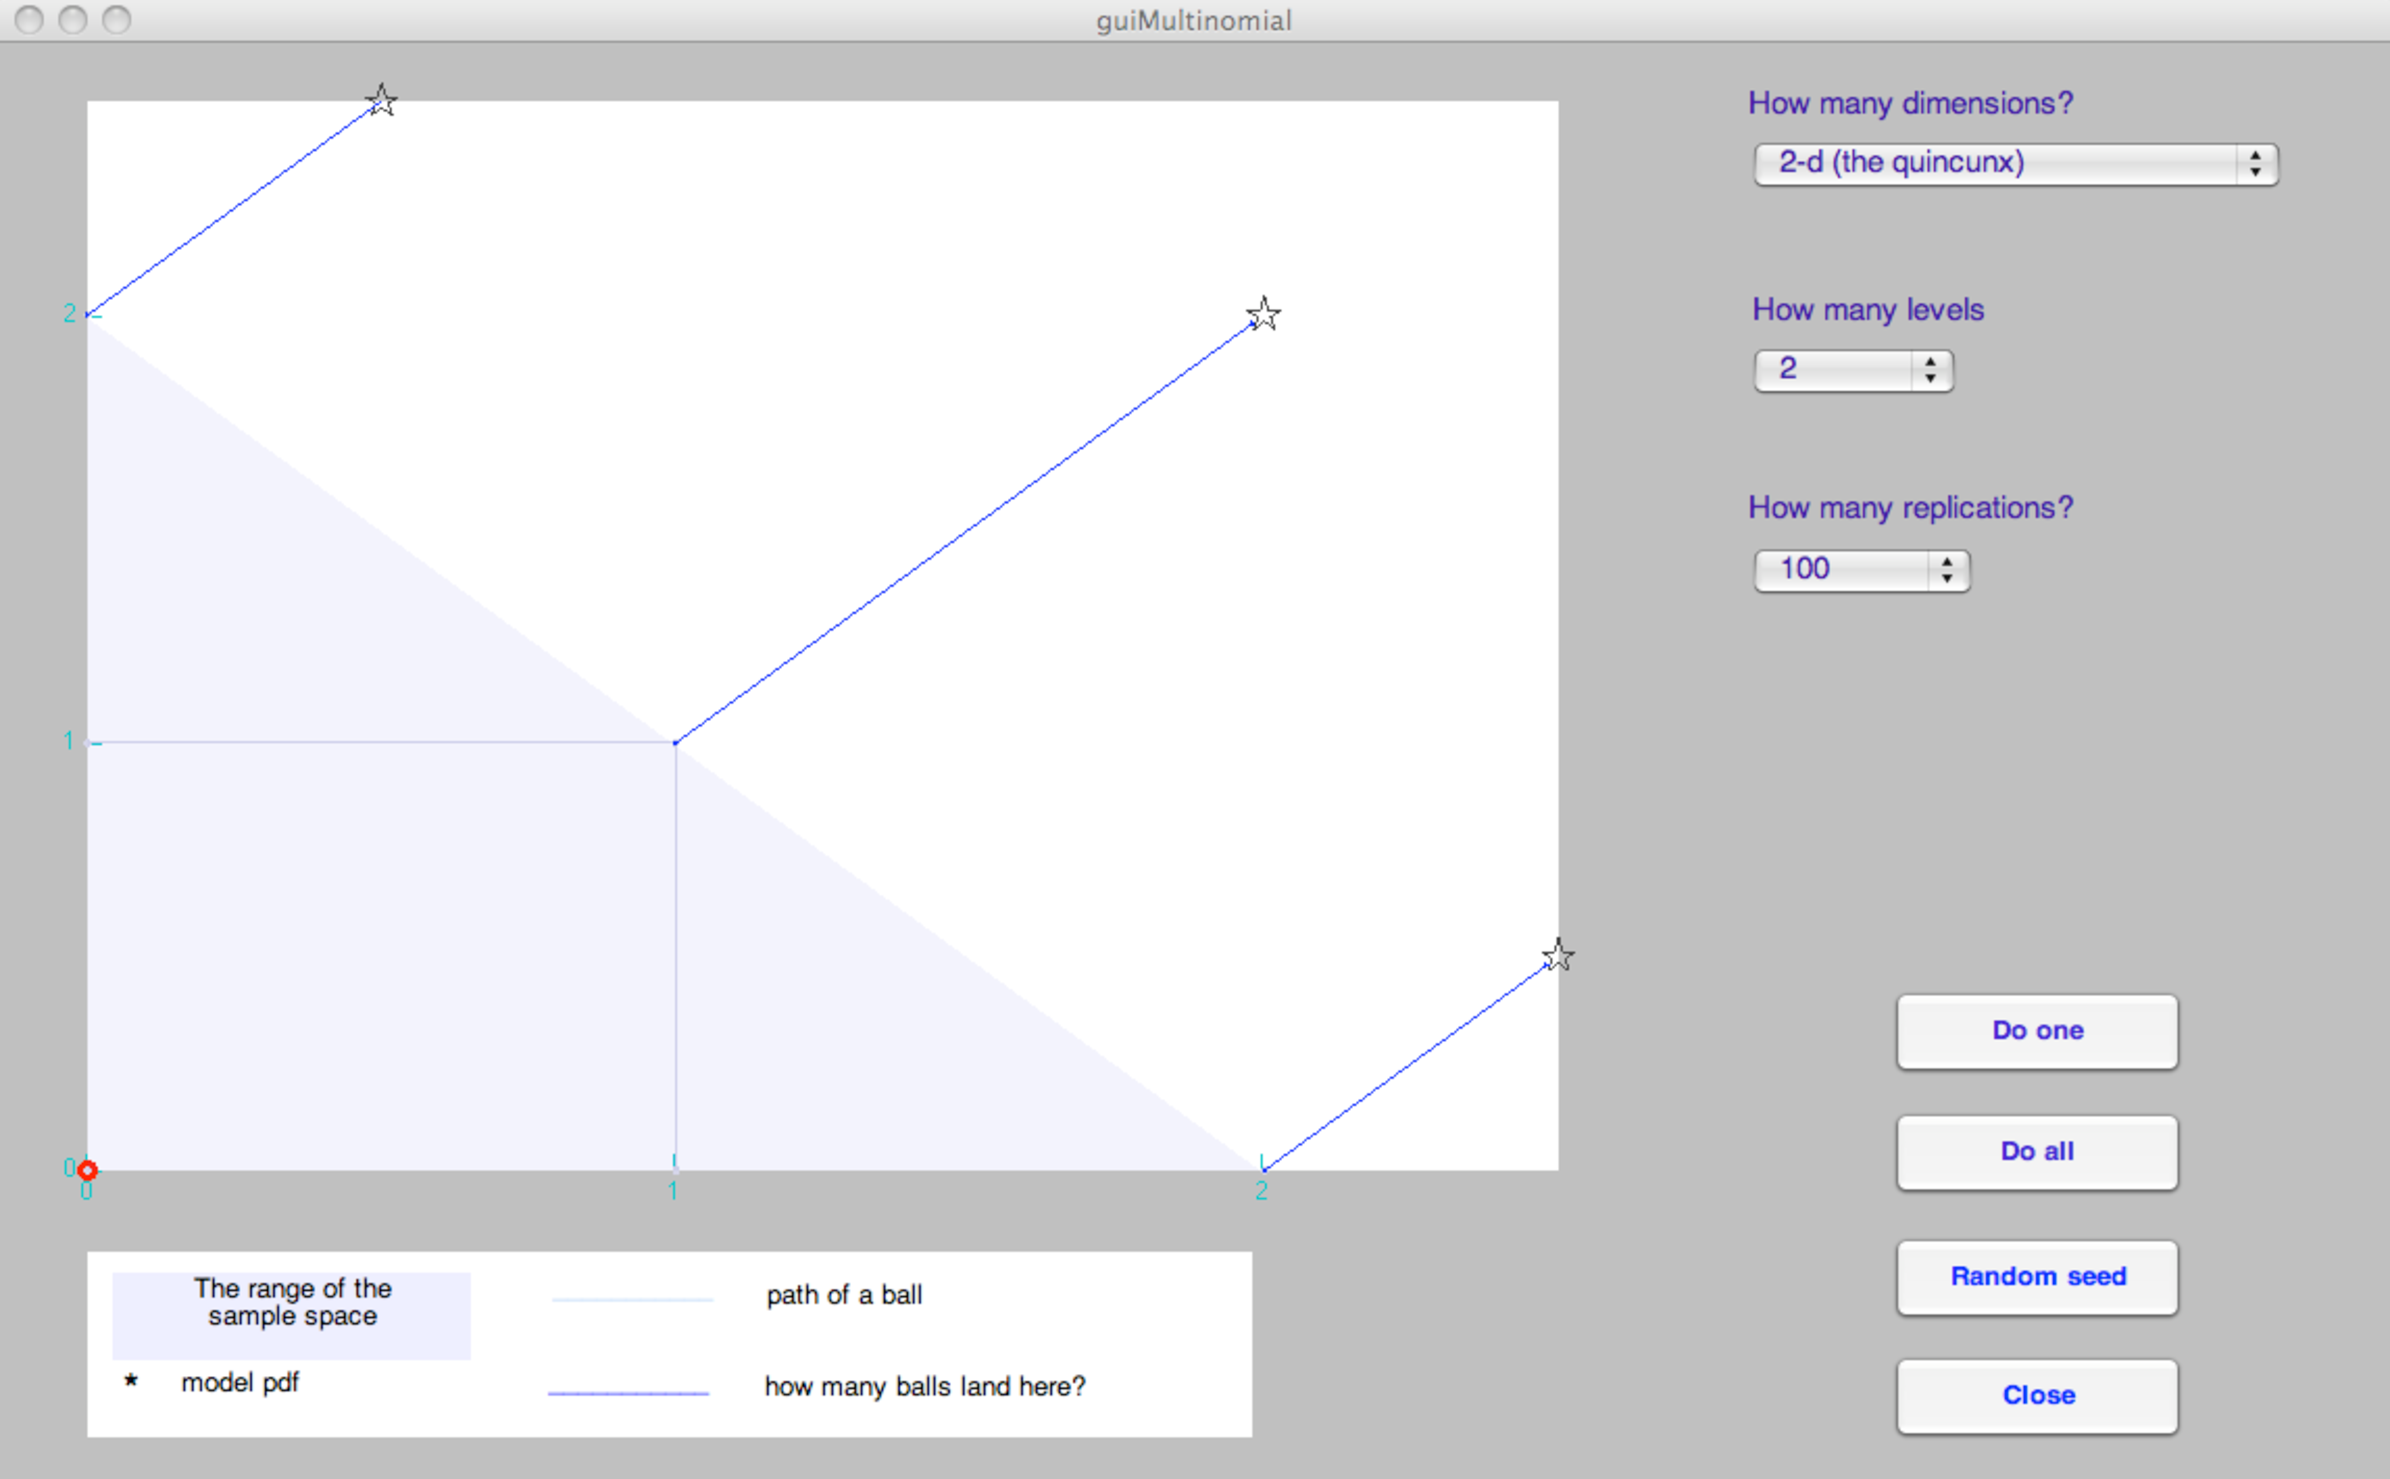
\includegraphics[width=6.50in]{figures/guiMultinomialQuincunx}}
\end{figure}
%}%end remove

We are now ready to extend the $\binomial(n,\theta)$ RV or \rv~to its multivariate version called the $\multinomial(n,\theta_1,\theta_2,\ldots,\theta_k)$ \rv.  We develop this \rv~as the sum of $n$ IID $\demoivre(\theta_1,\theta_2,\ldots,\theta_k)$ \rv~that is defined next.

\begin{model}[$\demoivre(\theta_1,\theta_2,\ldots,\theta_k)$ \rv]\label{M:deMoivreRVec}
The PMF of the $\demoivre(\theta_1,\theta_2,\ldots,\theta_k)$ \rv~$X := (X_1,X_2,\ldots,X_k)$ taking value $x := (x_1,x_2,\ldots,x_k) \in \{e_1,e_2,\ldots,e_k\}$, where the $e_i$'s are ortho-normal basis vectors in $\Rz^k$ is:
\[
f(x;\theta_1,\theta_2,\ldots,\theta_k) := \p(X=x) = \sum_{i=1}^k \theta_i \BB{1}_{\{e_i\}}(x) =
\begin{cases}
\theta_1 & \text{if} \quad x=e_1:=(1,0,\ldots,0) \in \Rz^k \\
\theta_1 & \text{if} \quad x=e_1:=(0,1,\ldots,0) \in  \Rz^k \\
\vdots \\
\theta_k & \text{if} \quad x=e_k:=(0,0,\ldots,1) \in  \Rz^k \\
0 & \text{otherwise}
\end{cases}
\]
Of course, $\sum_{i=1}^k \theta_i = 1$.
\end{model}

When we add $n$ IID $\demoivre(\theta_1,\theta_2,\ldots,\theta_k)$ \rv~together, we get the $\multinomial(n,\theta_1,\theta_2,\ldots,\theta_k)$ \rv~as defined below.

\begin{model}[$\multinomial(n,\theta_1,\theta_2,\ldots,\theta_k)$ \rv]\label{M:Multinomial}
We say that a \rv~$Y:=(Y_1,Y_2,\ldots,Y_k)$ obtained from the sum of $n$ IID $\demoivre(\theta_1,\theta_2,\ldots,\theta_k)$ \rv{s} with realisations
$$y:=(y_1,y_2,\ldots,y_k) \in \Yz:= \{(y_1,y_2,\ldots,y_k) \in \Zz_+^k : \sum_{i=1}^k y_i = n\}$$ has the PMF given by:
\[
f(y;n,\theta) := f(y;n,\theta_1,\theta_2,\ldots,\theta_k) := \p(Y=y;n,\theta_1,\theta_2,\ldots,\theta_k) = \binom{n}{y_1,y_2,\ldots,y_k} \prod_{i=1}^k \theta_i^{y_i} \ ,
\]
where, the multinomial coefficient:
\[
 \binom{n}{y_1,y_2,\ldots,y_k} := \frac{n!}{y_1! y_2! \cdots y_k!} \ .
\]
Note that the marginal PMF of $Y_j$ is $\binomial(n,\theta_j)$ for any $j=1,2,\ldots,k$.
\end{model}

\begin{figure}[htpb]
\caption{Septcunx on the Cartesian co-ordinates.  Simulations of $\multinomial(n=2,\theta_1=1/3,\theta_2=1/3,\theta_3=1/3)$ \rv~as the sum of $n$ IID $\demoivre(\theta_1=1/3,\theta_2=1/3,\theta_3=1/3)$ \rv{s} over $\{(1,0,0),(0,1,0),(0,0,1)\}$ with probabilities $\{\theta_1,\theta_2,\theta_3\}$, respectively.  The blue lines perpendicular to the sample space of the $\multinomial(3,\theta_1,\theta_2,\theta_3)$ \rv, i.e.~the plane in $\Rz^3$ connecting $(n,0,0)$, $(0,n,0)$ and $(0,0,n)$, are the density histogram of the samples.\label{F:MultinomSeptcunxn2n10r1000}}
\centering
\mbox{\subfigure[Thousand Samples with $n=2$]{\hspace{-2cm} 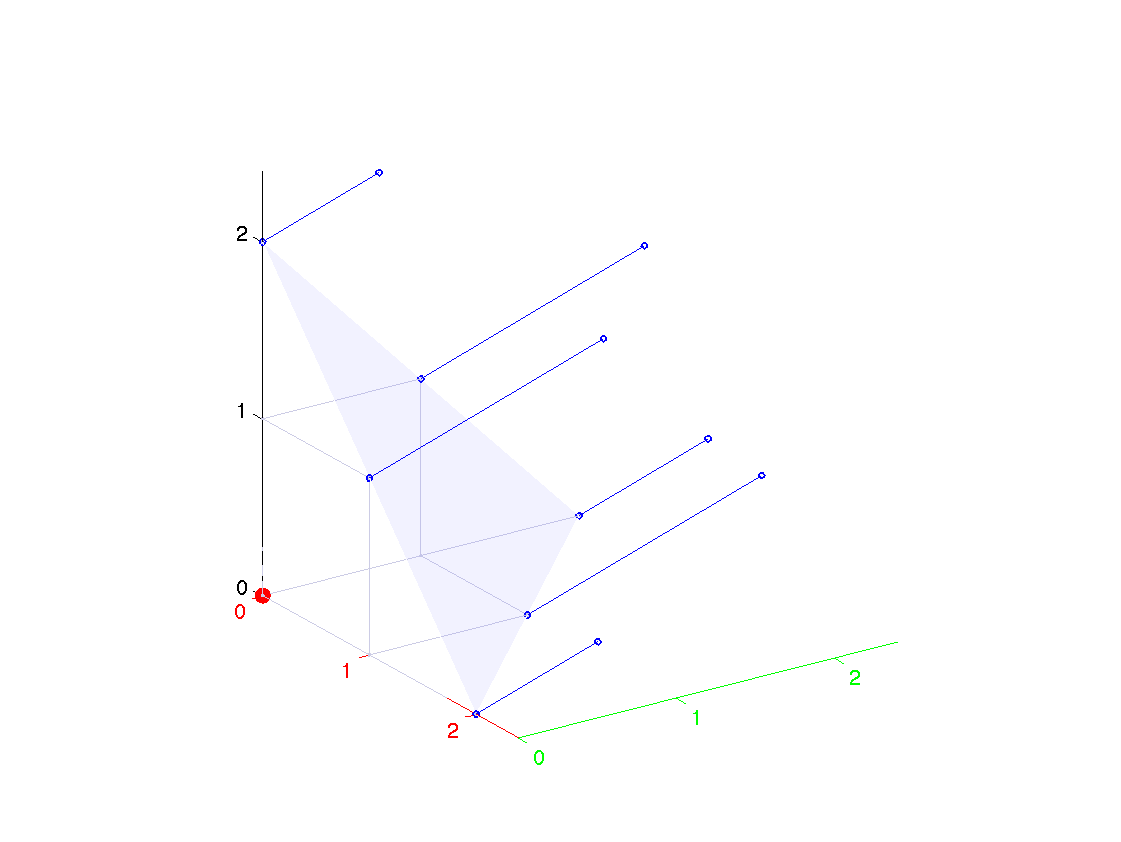
\includegraphics[width=4.250in]{figures/MultinomSeptcunxn2r1000}} \hspace{-2cm}
	   \subfigure[Thousand Samples with $n=10$]{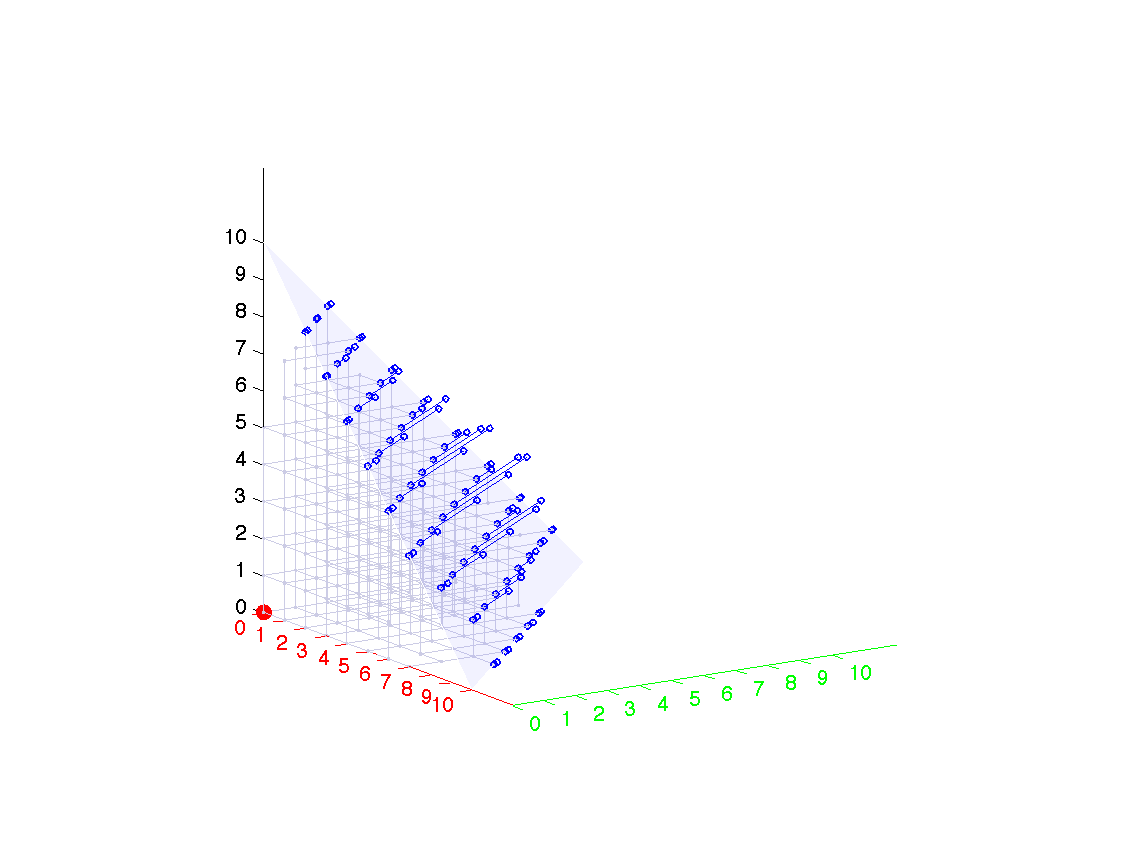
\includegraphics[width=4.250in]{figures/MultinomSeptcunxn10r1000}} }
\end{figure}

We can visualise the $\multinomial(n,\theta_1,\theta_2,\theta_3)$ process as a sum of $n$ IID $\demoivre(\theta_1,\theta_2,\theta_3)$ \rv{s} via a three dimensional extension of the Quincunx called the ``Septcunx'' and relate the number of paths that lead to a given trivariate sum $(y_1,y_2,y_3)$ with $\sum_{i-1}^3 y_i = n$ as the multinomial coefficient $\frac{n!}{y_1! y_2! y_3!}$.  In the Septcunx, balls choose from one of three paths along $e_1$, $e_2$ and $e_3$ with probabilities $\theta_1$, $\theta_2$ and $\theta_3$, respectively, in an IID manner at each of the $n$ levels, before they collect at buckets placed at the integral points in the $3$-simplex, $\Yz = \{(y_1,y_2,y_3) \in \Zz_+^3 : \sum_{i=1}^3 y_i=n \}$.  Once again, we can visualise that the sum of $n$ IID $\demoivre(\theta_1,\theta_2,\theta_3)$ \rv{s} constitute the $\multinomial(n,\theta_1,\theta_2,\theta_3)$ \rv~as depicted in \hyperref[F:MultinomSeptcunxn2n10r1000]{Figure \ref*{F:MultinomSeptcunxn2n10r1000}}.

%\remove{
\begin{labwork}[Septcunx Sampler Demo -- Sum of n IID $\demoivre(1/3,1/3,13/)$ \rv{s}]\label{LW:SeptcunxSampler}
Let us understand the Septcunx construction of the $\multinomial(n,1/3,1/3,1/3)$ \rv $X$ as the sum of $n$ independent and identical $\demoivre(1/3,1/3,13/)$ \rv{s} by calling the interactive visual cognitive tool as follows:
\begin{VrbM}
>> guiMultinomial
\end{VrbM}
The M-file {\tt guiMultinomial.m} will bring a GUI as shown in \hyperref[F:guiMultinomialQuincunx]{Figure \ref*{F:guiMultinomialQuincunx}}.  Using the drop-down menu at ``How many dimensions?'' change to ``3-d (the septcunx)'' and you will see a septcunx as shown in \hyperref[F:guiMultinomialSeptcunx]{Figure \ref*{F:guiMultinomialSeptcunx}}.  Next, using the drop-down menu at ``How many levels?'' change the number of levels to $2$ ($n=2$).  Now click the ``Do one'' button as many times as you like and comprehend the simulation process -- the path taken by the ball as it falls through two levels in three dimensional space.  Feel free to change the up-down and left-right sliders for the view angles.  Next, from the drop-down menu at ``How many  Replication?'' change it from $10$ to $100$.  You can press ``Do all'' to watch all 100 balls drop into their possible values at level $2$.  Change the number of levels or $n$ in $\multinomial(n,1/3,1/3,1/3)$ \rv to $5$ or $10$ and do more simulations until you are comfortable with the construction that the sum of $n$ IID $\demoivre(1/3,1/3,1/3)$ \rv{s} is the $\multinomial(n,1/3,1/3,1/3)$ \rv.
\end{labwork}

\begin{figure}[htpb]
\caption{Visual Cognitive Tool GUI: Septcunx.\label{F:guiMultinomialSeptcunx}}
\centering   \makebox{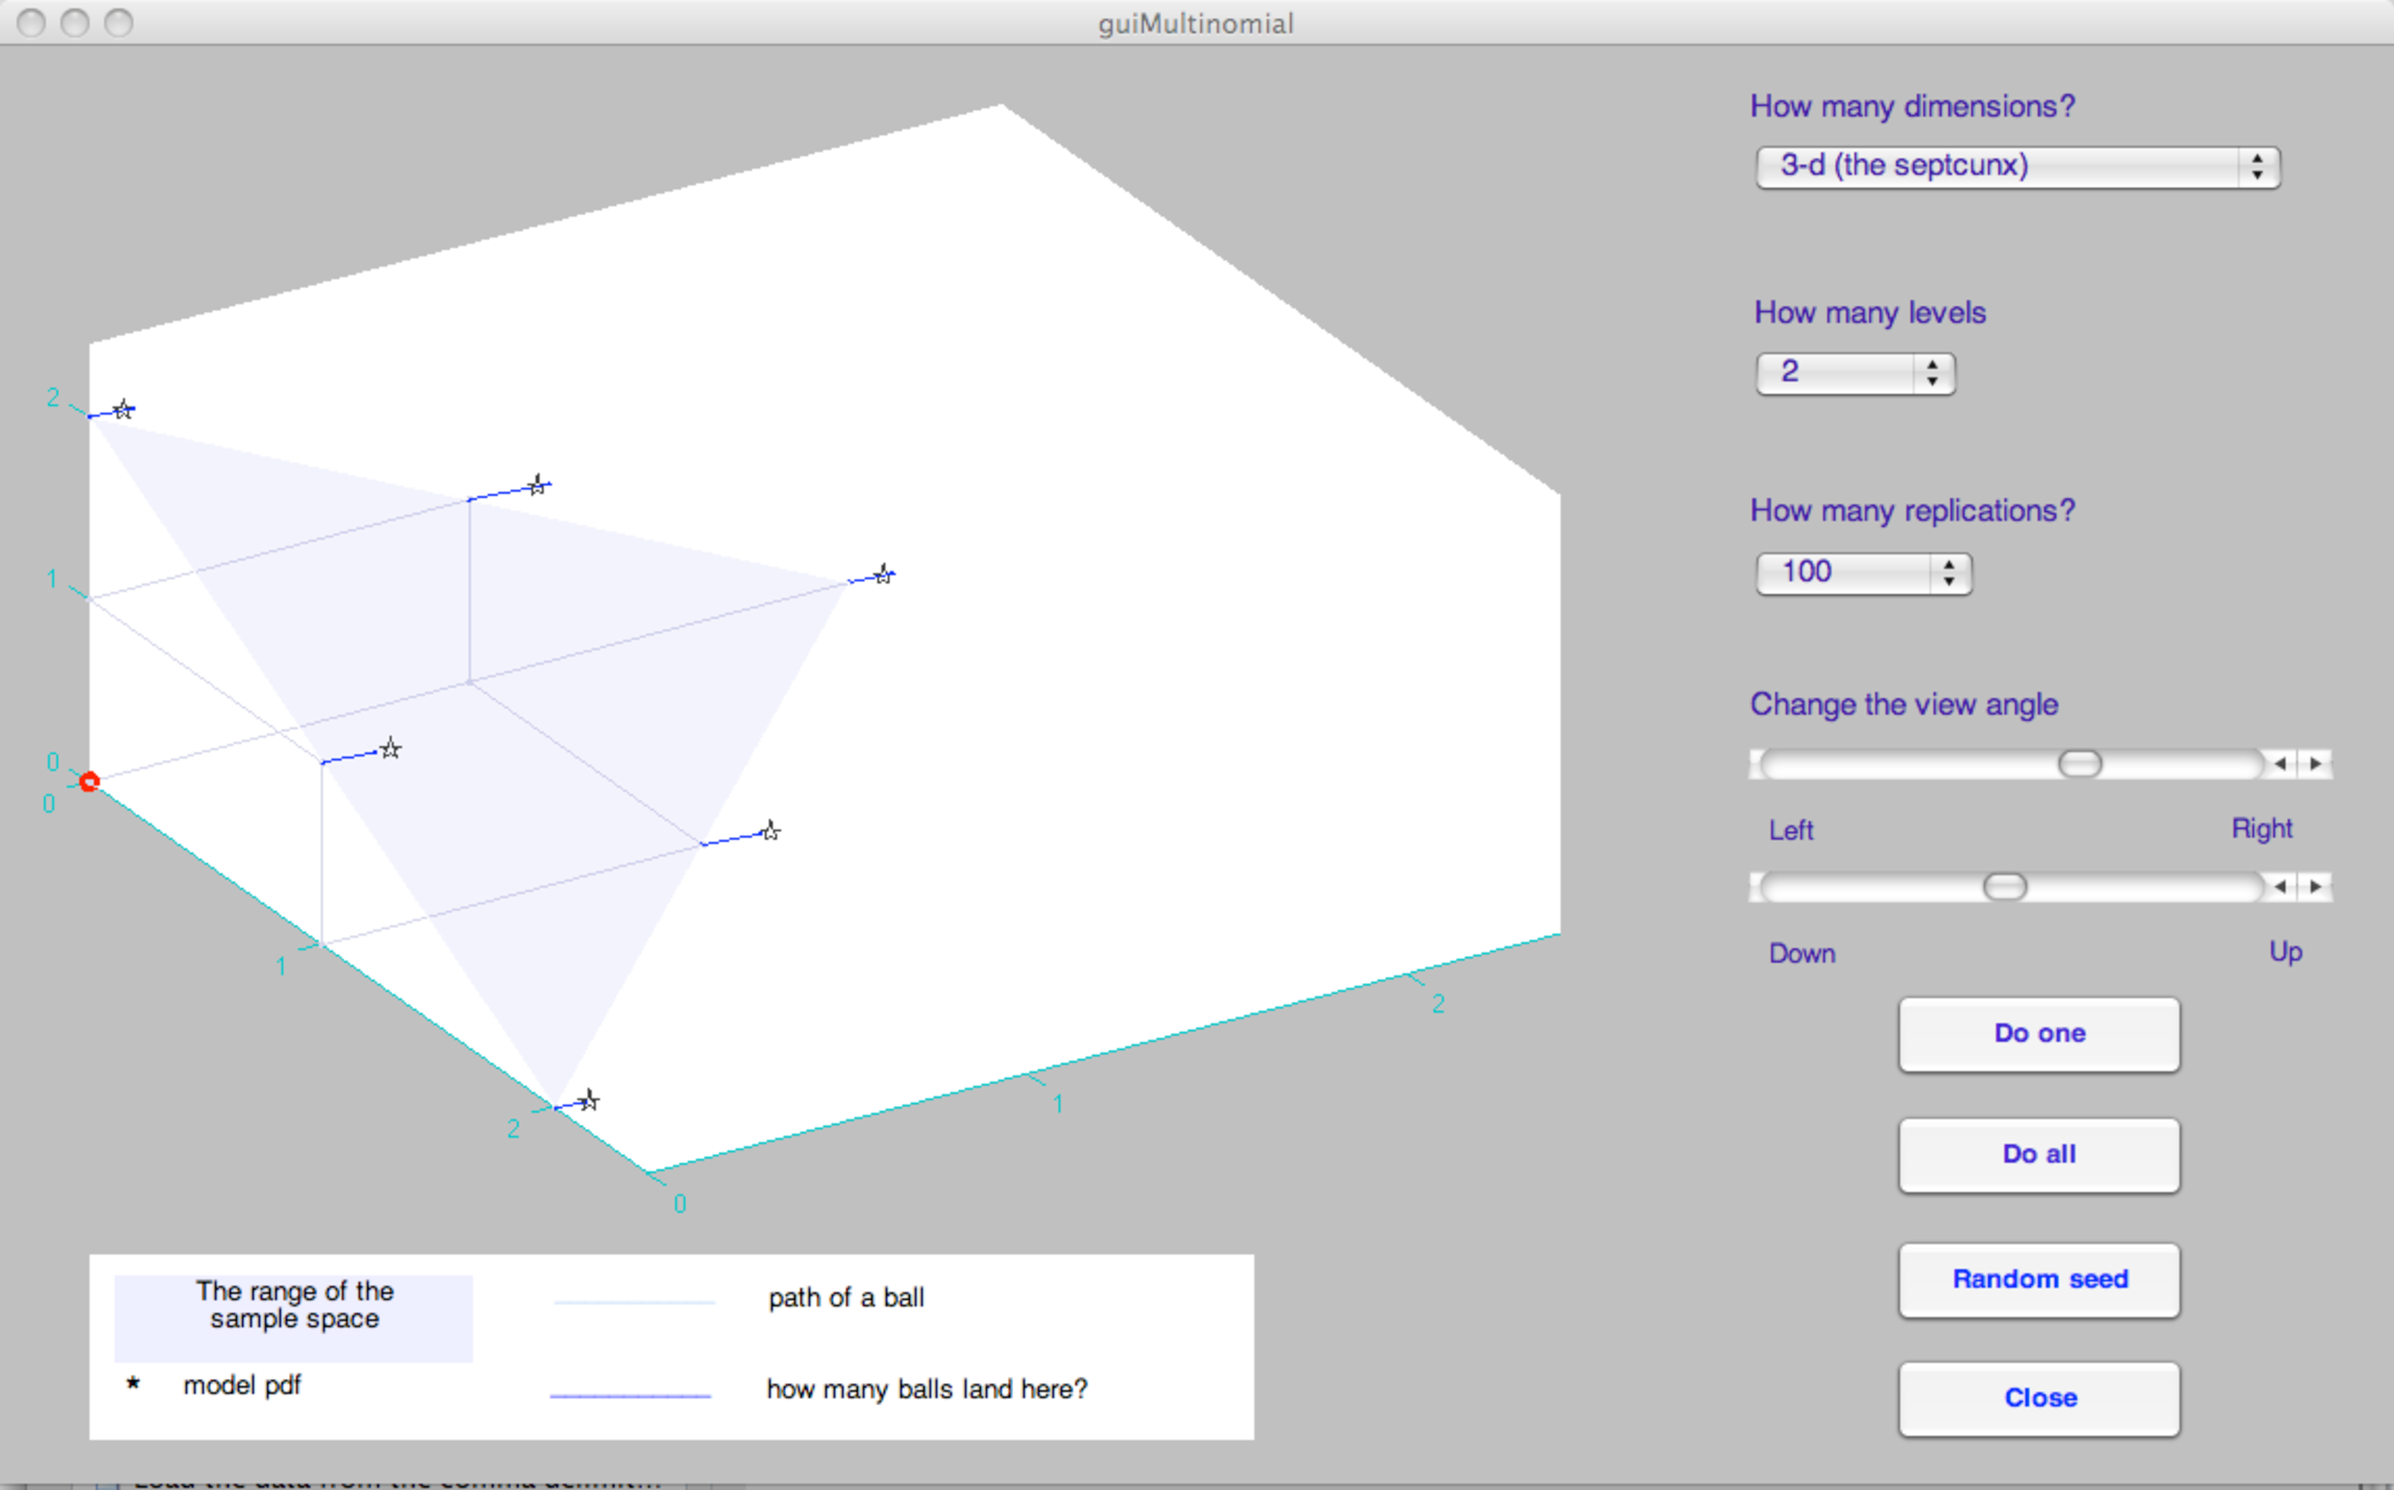
\includegraphics[width=6.50in]{figures/guiMultinomialSeptcunx}}
\end{figure}


\begin{labwork}[PDF of $\multinomial(n,\theta)$ \rv]\label{LW:MultinomialPdf}
We can implement the following \Matlab function {\tt MultinomialPdf} to compute the PDF of the $\multinomial(n,\theta)$ \rv~where $\theta:=(\theta_1,\theta_2,\ldots,\theta_k)$ is a point in the $k$-simplex $\bigtriangleup_k$ as follows:
\VrbMf[label=MultinomialPdf.m]{scripts/MultinomialPdf.m}
We can call this function to evaluate the PDF at a specific sample $x=(x_1,x_2,\ldots,x_k)$ as follows:
\begin{VrbM}
>> MultinomialPdf([2 0 0],2,[1/3 1/3 1/3])
ans =    0.1111
>> MultinomialPdf([0 2 0],2,[1/3 1/3 1/3])
ans =    0.1111
>> MultinomialPdf([0 0 2],2,[1/3 1/3 1/3])
ans =    0.1111
>> MultinomialPdf([1 1 0],2,[1/3 1/3 1/3])
ans =    0.2222
>> MultinomialPdf([1 0 1],2,[1/3 1/3 1/3])
ans =    0.2222
>> MultinomialPdf([0 1 1],2,[1/3 1/3 1/3])
ans =    0.2222
\end{VrbM}
\end{labwork}

\begin{simulation}[A simple multinomial simulation]\label{SIM:Multinomial}
Using the identity matrix $I$ in $\Rz^3$ that can be created in \Matlab using the {\tt eye(3)} command, and the $\demoivre(1/3,1/3,1/3)$ RV sampler, simulate vector-valued samples from $\demoivre(1/3,1/3,1/3)$ \rv.  Finally add up $n=10$ samples from $\demoivre(1/3,1/3,1/3)$ \rv~to produce samples from $\multinomial(10,1/3,1/3,1/3)$ \rv.
\end{simulation}

\section{von Neumann Rejection Sampler (RS)}\label{S:RS}
Rejection sampling [John von Neumann, 1947, in {\it Stanislaw Ulam 1909-1984}, a special issue of Los Alamos Science, Los Alamos National Lab., 1987, p.~135-136] is a Monte Carlo method to draw independent
samples from a target RV $X$ with probability density $f(x)$, where $x \in \Xz \subset \Rz^k$.  Typically, the target density $f$ is only known up to a constant and therefore the (normalised) density $f$ itself may be unknown and it  is difficult to generate samples directly from $X$.

Suppose we have another density or mass function $g$ for which the following are true:
\begin{asparaenum}[(a)]
\item	we can generate random variables from $g$;
\item	the support of $g$ contains the support of $f$, i.e.~$\Yz \supset \Xz$;
\item	a constant $a > 1$ exists, such that:
\begin{equation}
f(x)\leq ag(x).
\end{equation}
for any $x\in \Xz$, the support of $X$.  Then $x$ can be generated from Algorithm \ref*{A:RS}.
\end{asparaenum}

\begin{algorithm}
\caption{Rejection Sampler (RS) of von Neumann}
\label{A:RS}
\begin{algorithmic}[1]
\STATE {
{\it input:}
\begin{itemize}
\item[(1)] a target density $f(x)$,
\item[(2)] a proposal density $g(x)$ satisfying (a), (b) and (c) above.
\end{itemize}
}
\STATE {\it output:} a sample $x$ from RV $X$ with density $f$

\REPEAT
\STATE Generate $y \sim g$ and $u \sim \uniform(0,1)$
\UNTIL{$u \leq \frac{f(y)}{a g(y)}$}
\STATE {\it return:} $x \gets y$
\end{algorithmic}
\end{algorithm}

\begin{prop}[Fundamental Theorem of Simulation]  The von Neumann rejection sampler of Algorithm \ref*{A:RS} produces a sample $x$ from the random variable $X$ with density $f(x)$.
\begin{proof}
We shall prove the result for the continuous case. For any real number $t$:

\begin{eqnarray*}
F(t) &= \p(X \leq t) = \p\left(Y \leq t  \, | \, U \leq\frac{f(Y)}{ag(Y)} \right)
=\frac{\p\left(Y \leq t, U \leq\frac{f(Y)}{ag(Y)} \right)}{\p\left(U \leq\frac{f(Y)}{ag(Y)}\right)}\\
&=\frac{\int^t_{-\infty}\left(\int^{f(y)/ag(y)}_0 1 du\right)g(y)dy}{\int^{\infty}_{-\infty}\left(\int^{f(y)/ag(y)}_0 1 du\right)g(y)dy}
=\frac{\int^t_{-\infty}\left(\frac{f(y)}{ag(y)} \right)g(y)dy}{\int^{\infty}_{-\infty}\left(\frac{f(y)}{ag(y)} \right)g(y)dy}\\
&=\int^t_{-\infty}f(y)dy
\end{eqnarray*}
\end{proof}
\end{prop}

\begin{labwork}[Rejection Sampler Demo]\label{LW:guiRejectionsNormal01}
Let us understand the rejection sampler by calling the interactive visual cognitive tool:
\begin{VrbM}
>> guiRejections
\end{VrbM}
The M-file {\tt guiRejections.m} will bring a graphical user interface (GUI) as shown in \hyperref[F:guiRejectionsNormal01]{Figure \ref*{F:guiRejectionsNormal01}}.  Try various buttons and see how the output changes with explanations.  Try switching the ``Target distribution'' to ``Mywavy4'' and generate several rejection samples and see the density histogram of the accumulating samples.
\end{labwork}

\begin{figure}[htpb]
\caption{Visual Cognitive Tool GUI: Rejection Sampling from $X \sim \normal(0,1)$ with PDF $f$ based on proposals from $Y \sim \laplace(1)$ with PDF $g$.\label{F:guiRejectionsNormal01}}
\centering   \makebox{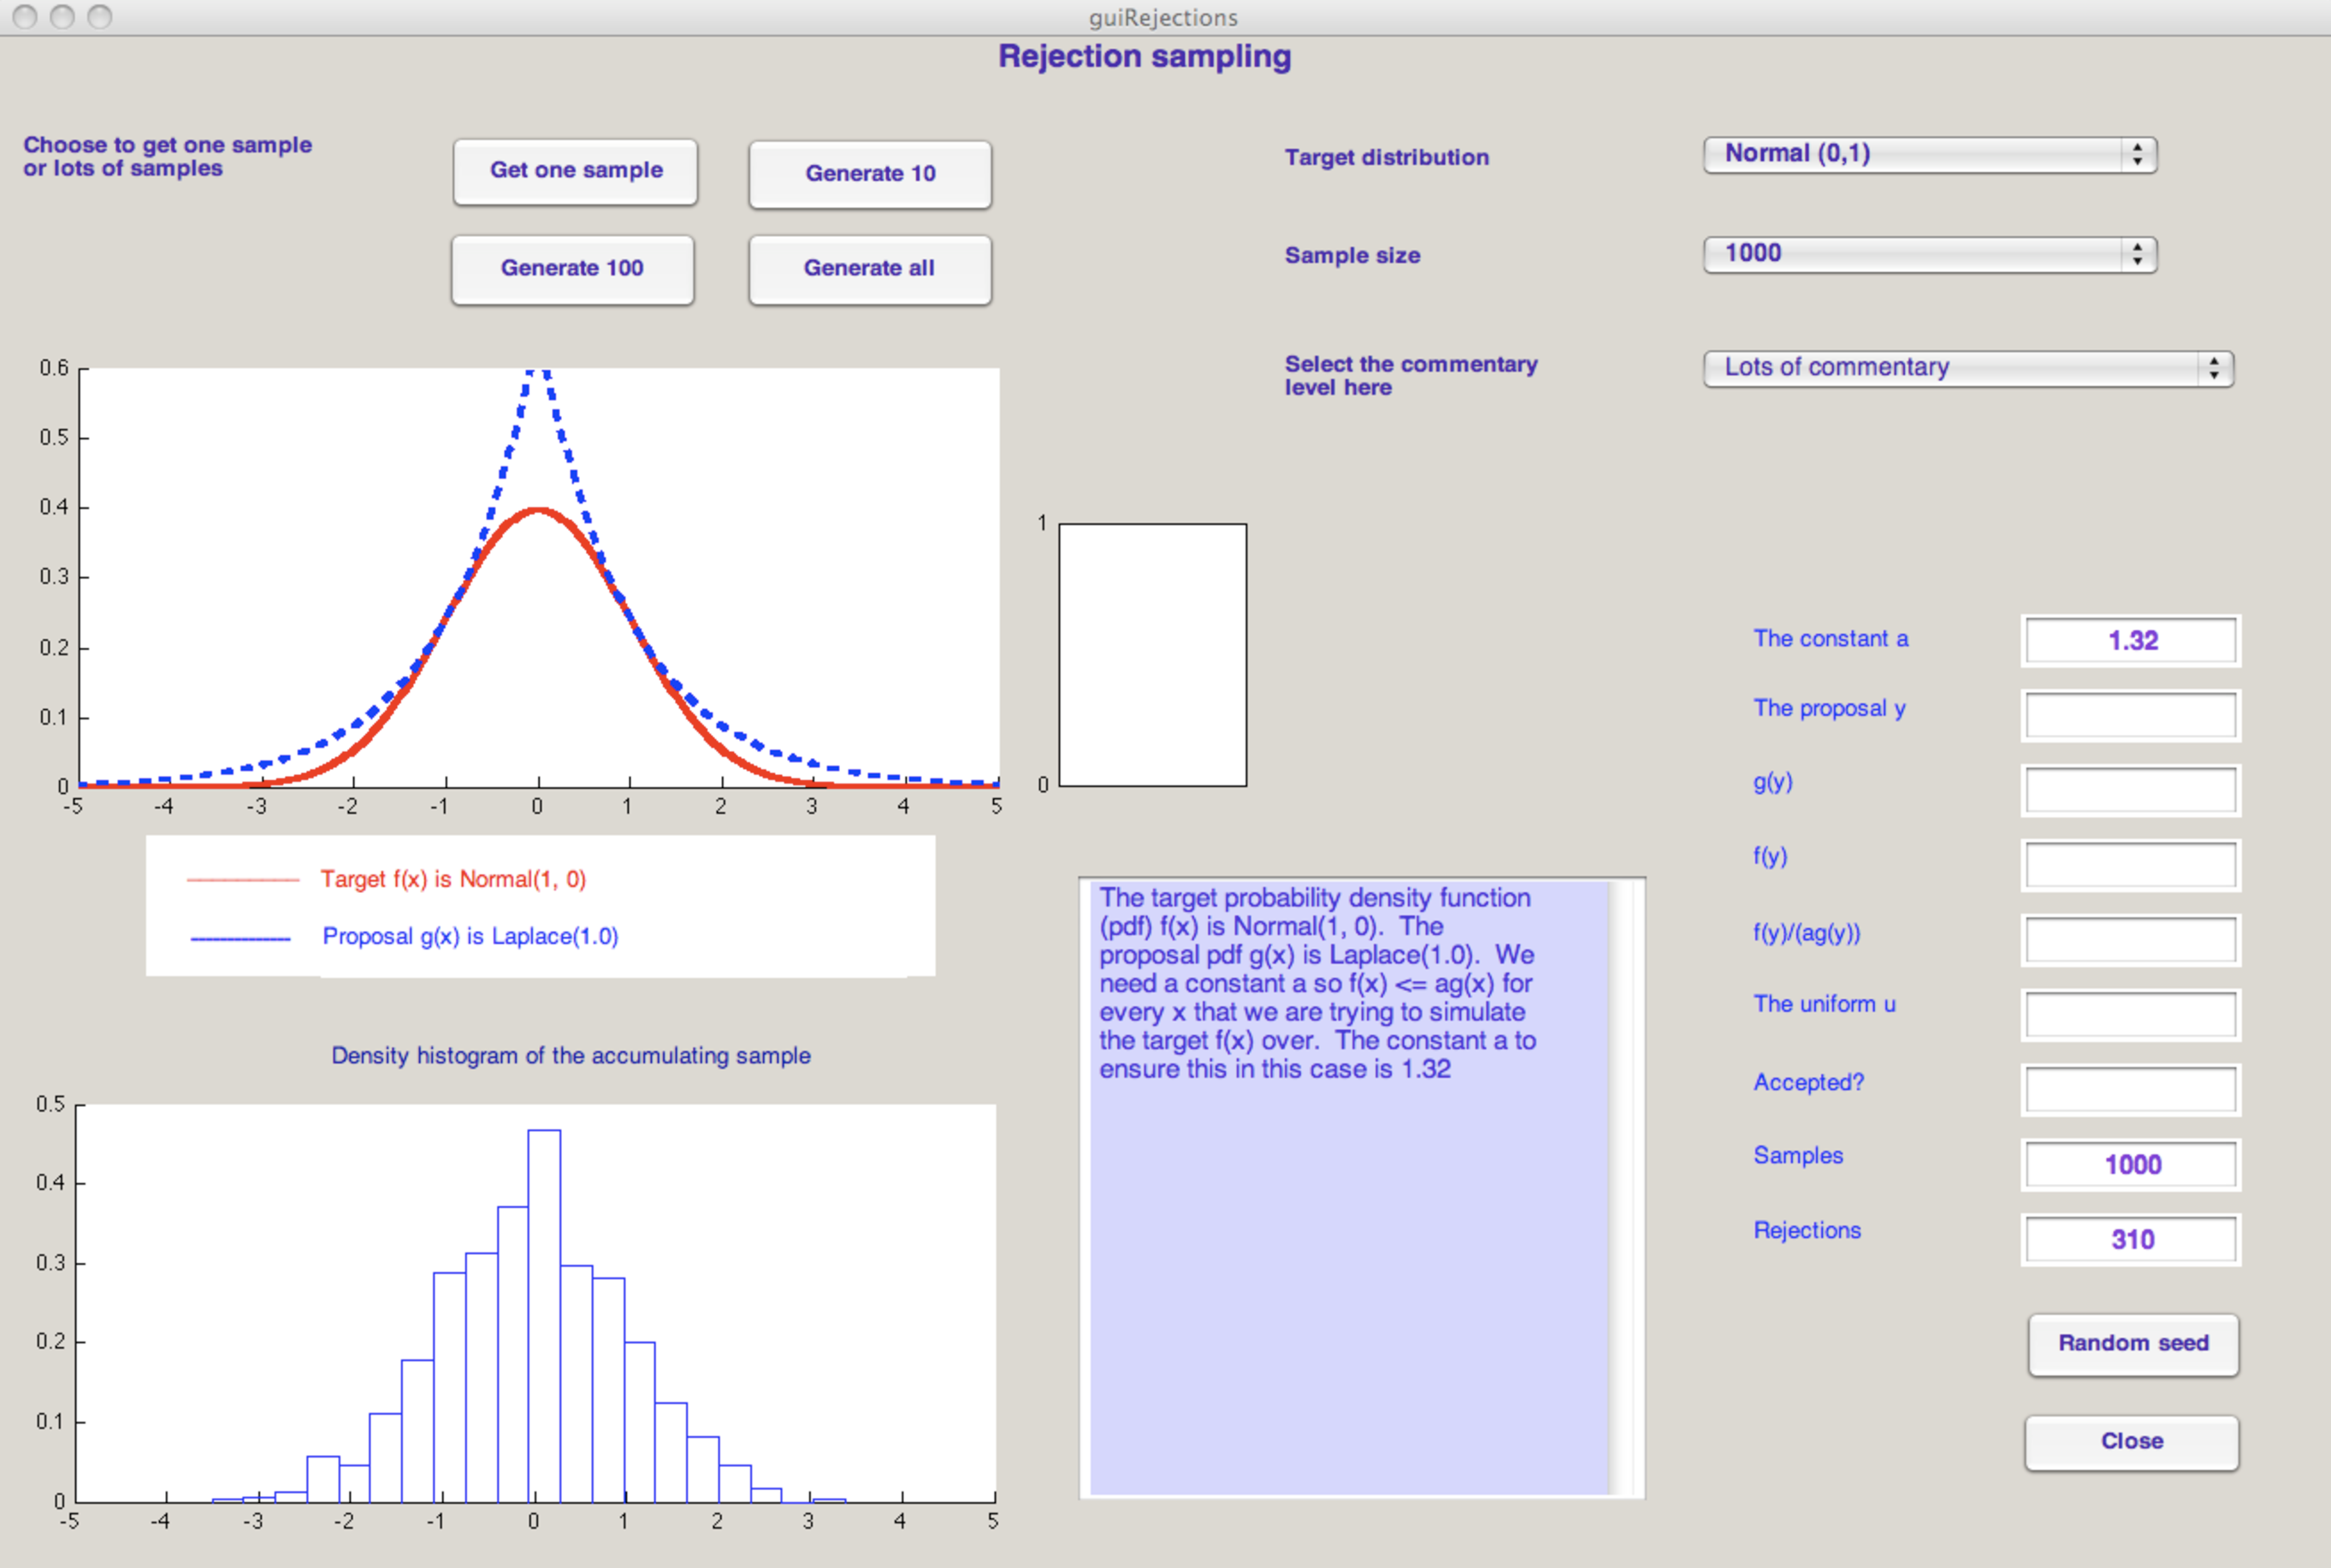
\includegraphics[width=6.50in]{figures/guiRejectionsNormal01}}
\end{figure}


%\subsection{\exmpl ({\tt rejection\_normal\_laplacian.m})}
% % Dominic's Demo needs Stats Toolbox
\begin{simulation}[Rejection Sampling $\normal(0,1)$ with $\laplace(1)$ proposals]\label{SIM:Normal01FromLaplace}
Suppose we wish to generate from $X \sim \normal(0, 1)$. Consider using the rejection sampler with proposals from $Y \sim \laplace(1)$ (using inversion sampler of \hyperref[SIM:Laplace]{Simulation \ref*{SIM:Laplace}}). The support of both RVs is $(-\infty,\infty)$. Next:
$$f(x)=\frac{1}{\sqrt{2\pi}}\exp\left(-\frac{x^2}{2}\right) \textrm{ and } g(x)=\frac{1}{2}\exp(-|x|)$$
and therefore:
$$\frac{f(x)}{g(x)}=\sqrt{\frac{2}{\pi}}\exp\left(|x|-\frac{x^2}{2}\right)\leq \sqrt{\frac{2}{\pi}}\exp\left(\frac{1}{2}\right) = a \approx 1.3155 \ .$$
Hence, we can use the rejection method with:
$$
\frac{f(y)}{a g(y)} = \frac{f(y)}{g(y)} \frac{1}{a} = \sqrt{\frac{2}{\pi}}\exp\left(|y|-\frac{y^2}{2}\right) \frac{1}{\sqrt{\frac{2}{\pi}}\exp\left(\frac{1}{2}\right)  } = \exp\left(|y|-\frac{y^2}{2} - \frac{1}{2} \right)
$$
%\includegraphics

Let us implement a rejection sampler as a function in the M-file {\tt RejectionNormalLaplace.m} by reusing the function in {\tt LaplaceInvCDF.m}.
\VrbMf[label=RejectionNormalLaplace.m]{scripts/RejectionNormalLaplace.m}
We may obtain a large number of samples an plot them as a histogram using the following commands:
\begin{VrbM}
>> % use funarray to convert 1000 zeros into samples from the Normal(0,1)
>> y=arrayfun(@(x)(RejectionNormalLaplace()),zeros(1,1000));
>> hist(y,20) % histogram with 20 bins
\end{VrbM}
\end{simulation}

\begin{figure}[htpb]
\caption{Rejection Sampling from $X \sim \normal(0,1)$ with PDF $f$ based on  100 proposals from $Y \sim \laplace(1)$ with PDF $g$.\label{F:RSNormalLaplace}}
\centering   \makebox{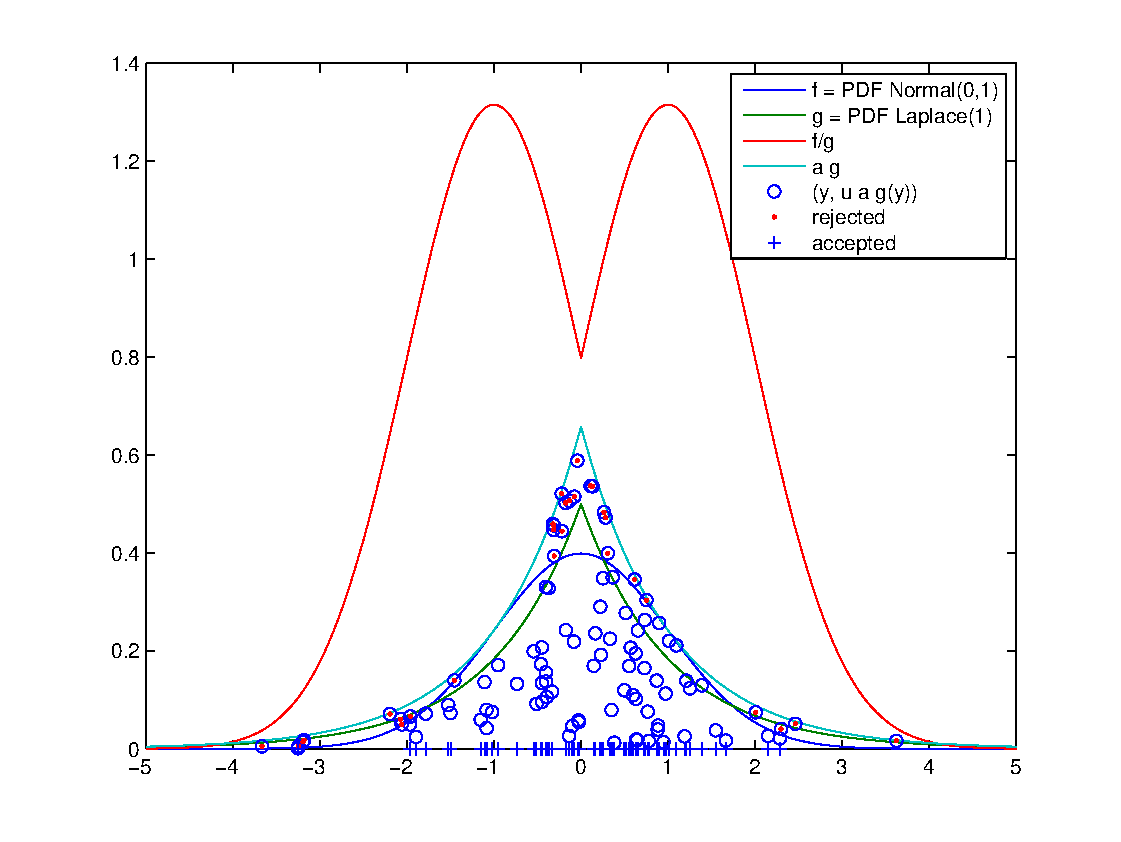
\includegraphics[width=4.50in]{figures/RSNormalLaplace}}
\end{figure}

\begin{classwork}[A note on the proposal's tail in rejection sampling]
The condition $f(x)\leq ag(x)$ is equivalent to $f(x)/g(x)\leq a$, which says that $f(x)/g(x)$ must be bounded; therefore, $g$ must have higher tails than $f$.
The rejection method cannot be used to generate from a Cauchy distribution using a normal distribution, because the latter has lower tails than the former.
\end{classwork}

%\includegraphics

The next result tells us how many iterations of the algorithm are needed, on average, to get a sample value from a RV with PDF $f$.

\begin{prop}[Acceptance Probability of RS] The expected number of iterations of the rejection algorithm to get a sample $x$ is the constant $a$.

\begin{proof}
For the continuous case:
\begin{displaymath}
\p(\textrm{`accept }y\textrm{'})=\p\left( u\leq \frac{f(y)}{ag(y)}\right)=\int^{\infty}_{-\infty}\left(\int^{f(y)/ag(y)}_0du\right)g(y)dy=\int^{\infty}_{-\infty}\frac{f(y)}{ag(y)}g(y)dy=\frac{1}{a}.
\end{displaymath}
And the number of proposals before acceptance is the $\geometric(1/a)$ RV with expectation $\frac{1}{1/a}=a$.
\end{proof}
\end{prop}

The closer $ag(x)$ is to $f(x)$, especially in the tails, the closer $a$ will be to 1, and hence the more efficient the rejection method will be.

The rejection method can still be used only if the un-normalised form of $f$ or $g$ (or both) is known. In other words, if we use:
$$f(x)=\frac{\tilde{f}(x)}{\int \tilde{f}(x)dx} \textrm{ and } g(x)=\frac{\tilde{g}(x)}{\int \tilde{g}(x)dx} $$
we know only $\tilde{f} (x)$ and/or $\tilde{g}(x)$ in closed-form.  Suppose the following are satisfied:
\begin{asparaenum}[(a)]
\item	we can generate random variables from $g$;
\item	the support of $g$ contains the support of $f$, i.e.~$\Yz \supset \Xz$;
\item	a constant $\tilde{a} > 0$ exists, such that:
\begin{equation}
\tilde{f}(x)\leq\tilde{a}\tilde{g}(x),
\end{equation}
for any $x\in \Xz$, the support of $X$.  Then $x$ can be generated from Algorithm \ref*{A:RS2}.
\end{asparaenum}

\begin{algorithm}
\caption{Rejection Sampler (RS) of von Neumann -- target shape}
\label{A:RS2}
\begin{algorithmic}[1]
\STATE {
{\it input:}
\begin{itemize}
\item[(1)] shape of a target density $\tilde{f}(x) = \left({\int \tilde{f}(x)dx}\right) f(x)$,
\item[(2)] a proposal density $g(x)$ satisfying (a), (b) and (c) above.
\end{itemize}
}
\STATE {\it output:} a sample $x$ from RV $X$ with density $f$

\REPEAT
\STATE Generate $y \sim g$ and $u \sim \uniform(0,1)$
\UNTIL{$u\leq\frac{\tilde{f}(y)}{\tilde{a}\tilde{g}(y)}$}
\STATE {\it return:} $x \gets y$
\end{algorithmic}
\end{algorithm}
Now, the expected number of iterations to get an $x$ is no longer $\tilde{a}$ but rather the integral ratio: $$ \left( \frac{\int_{\Xz} \tilde{f}(x) dx }{\int_{\Yz} \tilde{a} \tilde{g}(y) dy} \right)^{-1} \ .$$

%%The problem is already difficult for the stretched oscillating density for example.
%\begin{figure}
%\centering   \makebox[10pt]{
%\input{pqfRSMH.tex}
%}
%\caption{The characteristics of three samplers with target $p = p^*/N_p$: (1) Rejection sampler with
%proposal $q=q^*/N_q$ and the envelope function $f_q$, (2) an independent
%Metropolis-Hastings sampler (IMHS) driven by an independent base chain $I$
%with proposal $q_I = q^*_I / N_{q^*_I}$ and (3) a local Metropolis-Hastings sampler (LMHS)
%driven by a local base chain $L$ with proposal $q_L = q^*_L / N_{q^*_L}$
%centered at the current state (open square at the bottom). \label{F:RSMH}}
%\end{figure}
%Rejection Sampling from $Normal(\mu,\sigma^2)$ RV $X$ using proposals from $Cauchy(\nu)$
%\begin{model}[Cauchy]
%A RV $X$ is said to be $Cauchy(\nu)$ distributed if:
%\[
%f(x;\nu) = \frac{\nu}{\pi(x^2+\nu^2)}, \qquad F(x;\nu) = \frac{1}{2} +\frac{1}{\pi} \arctan\left(\frac{x}{\nu}\right), \qquad F^{[-1]}(u;\nu) = \nu \tan \left(\pi \left( u- \frac{1}{2} \right) \right)
%\]
%\end{model}
%\begin{labwork}
%Implement the inversion sampler to draw samples from the $Cauchy(\nu)$ RV.
%\end{labwork}

The {\bf Ziggurat Method} [G.~Marsaglia and W.~W.~Tsang, SIAM Journal of Scientific and Statistical Programming, volume 5, 1984] is a rejection sampler that can efficiently draw samples from the $Z \sim \normal(0,1)$ RV.  The \Matlab function {\tt randn} uses this method to produce samples from $Z$.  See  \href{http://www.mathworks.com/company/newsletters/news_notes/clevescorner/spring01_cleve.html}{\url{http://www.mathworks.com/company/newsletters/news_notes/clevescorner/spring01_cleve.html}} or \href{http://en.wikipedia.org/wiki/Ziggurat_algorithm}{\url{http://en.wikipedia.org/wiki/Ziggurat_algorithm}} for more details.

\begin{labwork}[Gaussian Sampling with {\tt randn}]\label{LW:randn}
We can use \Matlab function {\tt randn} that implements the Ziggurat method to draw samples from an RV $Z \sim \normal(0,1)$ as follows:
\begin{VrbM}
>> randn('state',67678); % initialise the seed at 67678 and method as Ziggurat -- TYPE help randn
>> randn % produce 1 sample from Normal(0,1) RV
ans =    1.5587
>> randn(2,8) % produce an 2 X 8 array of samples from Normal(0,1) RV
ans =
    1.2558    0.7834    0.6612    0.3247    0.1407    1.0562    0.8034    1.2970
   -0.5317    0.0417   -0.3454    0.6182   -1.4162    0.4796   -1.5015    0.3718
\end{VrbM}
If we want to produce samples from $X \sim \normal(\mu,\sigma^2)$ with some user-specified $\mu$ and $\sigma$, then we can use the following relationship between $X$ and $Z \sim \normal(0,1)$:
\[
X \gets \mu + \sigma Z, \qquad Z \sim \normal(0,1) \ .
\]
Suppose we want samples from $X \sim \normal(\mu=\pi, \sigma^2=2)$, then we can do the following:
\begin{VrbM}
>> randn('state',679); % initialise the seed at 679 and method as Ziggurat -- TYPE help randn
>> mu=pi % set the desired mean parameter mu
mu =    3.1416
>> sigma=sqrt(2) % set the desired standard deviation parameter sigma
sigma =    1.4142
>> mu + sigma * randn(2,8) % produces a 2 X 8 array of samples from Normal(3.1416,1.4.42)
ans =
    1.3955    1.7107    3.9572    3.2618    6.1652    2.6971    2.4940    4.5928
    0.8442    4.7617    3.5397    5.0282    1.6139    5.0977    2.0477    2.3286
\end{VrbM}
\end{labwork}

%%% new content added on 28 Dec 2010: Raaz to integrate and streamline
%%% this may be used as labwork or exercise, i am calling it labwork for now
\begin{labwork}[Sampling from truncated normal distributions] [Christian P. Robert, Simulation of truncated normal variables, Statistics and Computing (1995) 5, 121-125]
Let $N_+(\mu,\tau,\sigma^2)$ denote the left-truncated normal distribution with truncation point $\tau$ and density given by

$$f(x|\mu,\tau,\sigma^2)=\frac{exp(-(x-\mu)^2/2\sigma^2)}{\sqrt{2\pi}\sigma[1-\Phi((\tau-\mu)/\sigma)]}\BB{1}_{x\geq\tau}.$$

When $\tau<\mu$, the rejection sampler can readily be used to simulate from $N_+(\mu,\tau,\sigma^2)$ by simulating from $\normal(\mu,\sigma^2)$ until a number larger than $\tau$ is obtained. When $\tau>\mu$, however, this can be inefficient and increasingly so as $\tau$ gets further out into the right tail. In this case, a more efficient approach is to use the rejection sampler with the following translated exponential distribution as the proposal distribution:

$$g(y|\lambda,\tau)={\lambda}exp(-\lambda(y-\tau))\BB{1}_{y\geq\tau}.$$

\begin{enumerate}
\item Show that for simulating from $N_+(\mu=0,\tau,\sigma^2=1)$ when $\tau\geq0$, the best choice of $\lambda$ that maximizes the expected acceptance probability for the rejection sampler is given by
$$\lambda=\frac{\tau+\sqrt{\tau^2+4}}{2}$$
\item Find the maximum expected acceptance probabilities for the following truncation points, $\tau=0,0.5,1,1.5,2,2.5$ and 3. What can you conclude about efficiency as $\tau$ gets further out into the right tail?
\item Describe how samples from $N_+(\mu,\tau,\sigma^2)$ can be obtained by simulating from $N_+(\mu=0,\tau,\sigma^2=1)$ and using location-scale transformation.
\item A related distribution, denoted by $N_-(\mu,\tau,\sigma^2)$, is the right-truncated normal distribution truncated on the right at $\tau$. Describe how samples from $N_-(\mu,\tau,\sigma^2)$ can be obtained by simulating from an appropriate left-truncated normal distribution.
\item Write a \Matlab function that provides samples from a truncated normal distribution. The function should have the following inputs: number of samples required, left or right truncation, $\mu$, $\sigma^2$ and $\tau$.
\end{enumerate}
\end{labwork}

%%% begin Dominic's Material
%%% WORK: We need to introduce sampling from a large discrete distribution, say the Alias method before this material % theoretically explain randsample function in Matlab
\section{Importance Resampler}
The rejection method cannot be used when the constant $a$ or $\tilde{a}$ that guarantees the envelape condition cannot be found. The importance resampler, also known as the method of {sampling/importance resampling}, does not require the constant, but it produces a random variable that is only approximately distributed according to $f$. As for the rejection method, we need a density/mass function $g$ that we can generate from and that has support at least as large as the support of $f$.

\begin{algorithm}
\caption{Importance Resampler}
\label{A:ImpReSampler}
\begin{algorithmic}[1]
\STATE {
{\it input:}
\begin{itemize}
\item[(1)] shape of a target density $\tilde{f}(x) = \left({\int \tilde{f}(x)dx}\right) f(x)$,
\item[(2)] a proposal density $g(x)$ satisfying only (a) and (b) above.
\item[(3)] a large enough integer $m$.
\end{itemize}
}
\STATE {\it output:} a sample $x{\prime}$ from RV $X^{\prime}$ with density $f^{\prime}$ that is close to  $f$
\STATE Generate $y_1,\ldots, y_m \sim g$
\STATE Compute
$$
w_i=\frac{f(y_i)/g(y_i)}{\sum^m_{j=1}f(y_j)/g(y_j)},i=1,\ldots,m \enspace .
$$
\STATE Resample $x^{\prime}$ from $\{y_1,\ldots, y_m\}$ with weights $\{w_1,\ldots, w_m\}$
\end{algorithmic}
\end{algorithm}

\begin{prop}The Importance Resampler of Algorithm~\ref{A:ImpReSampler} produces samples from a variable $X^{\prime}$ that is approximately distributed according to $f$, in the sense that:
\begin{equation}
\lim_{m\rightarrow \infty}\p( X^{\prime} \leq t)=\int^t_{-\infty}f(x)dx
\end{equation}
for any real number $t$.
\begin{proof}
\begin{displaymath}
\begin{split}
&\p(X^{\prime}\leq t)=\sum^m_{i=1}w_iI_{(-\infty,t]}(y_i)=\frac{\frac{1}{m}\sum^m_{i=1}\frac{f(y_i)}{g(y_i)}I_{(-\infty,t]}(y_i)}{\frac{1}{m}\sum^m_{i=1}\frac{f(y_i)}{g(y_i)}}\\
%\end{displaymath}
%\begin{displaymath}
&\underrightarrow{^{m\rightarrow\infty}}\frac{E [\frac{f(y)}{g(y)}I_{(-\infty,t]}(y)]}{E[\frac{f(y)}{g(y)}]}=\frac{\int^t_{-\infty}f(y)dy}{{\int^{\infty}_{-\infty}f(y)dy}}=\int^t_{-\infty}f(y)dy\\
\end{split}
\end{displaymath}
\end{proof}
\end{prop}

Let us visualise the Importance Resampler in action from \hyperref[Mf:ImpResamplerCauchyViaNormal]{Labwork~\ref*{Mf:ImpResamplerCauchyViaNormal}}.

\begin{labwork}[$\cauchy$ RV via Importance Resampler]
Use the sampling/importance resampling method to generate $1000$ approximate $\cauchy$ samples  by using the $\normal(0,1)$ samples:

$$f(x)=\frac{1}{\pi(1+x^2)} \textrm{ and  } g(x)=\frac{1}{\sqrt{2\pi}}\exp\left(-\frac{x^2}{2}\right).$$

\begin{VrbM}
n = 1000;
m = 10000;
y = randn(1,m); % randn is the N(0,1) generator in Matlab
y2 = y .* y;
w = exp(0.5 * y2) ./ (1 + y2);
w = w / sum(w);
x = randsample(y,n,true,w); % resample n values from y weighted by w
\end{VrbM}
\end{labwork}

Note that to get $n$ sample points from $f$ using sampling/importance resampling, we must start with a sample from $g$ of size $m$ larger than $n$.

As for the rejection method, the sampling/importance resampling method can still be used if only the un-normalised form of $f$ or $g$ (or both) is known, simply by using the un-normalised densities/mass functions to compute the weights.
%%%%%%end Dominic's material

\section{Other Continuous Random Variables}\label{S:OtherContRVs}
Here, we see other common continuous RVs that can be simulated from transforming RVs we have already encountered.
%}%end remove
%\remove{
\begin{simulation}[$\gammA(\lambda,k)$ for integer $k$]\label{SIM:Gamma}
Using this relationship we can simulate from $X \sim \gammA(\lambda,k)$, for an integer-valued $k$, by simply summing $k$ IID samples from $\exponential(\lambda)$ RV as follows:
\begin{VrbM}
>> lambda=0.1; %declare some lambda parameter
>> k=5; % declare some k parameter (has to be integer)
>> rand('twister',7267); % initialise the fundamental sampler
>> % sum k IID Exponential(lambda) samples for one desired sample from Gamma(lambda,k)
>> x= sum(-1/lambda*log(rand(k,1)))
x =   28.1401
>> % sum the 10 columns of k X 10 IID Exponential(lambda) samples for 10 desired samples from Gamma(lambda,k)
>> x= sum(-1/lambda*log(rand(k,10)))
x =
   83.8150   61.2674   80.3683  103.5748   48.4454   20.2269   93.8310   56.1909   77.0656   29.0851
\end{VrbM}
\end{simulation}

\begin{model}[$\lognormal(\lambda,\zeta)$]
$X$ has a $\lognormal(\lambda,\zeta) $ distribution if $\log(X)$ has a $\normal(\lambda,\zeta^2)$ distribution.  The location parameter $\lambda = \e(\log(X)) > 0$ and the scale parameter $\zeta > 0$.  The PDF is:
\begin{equation}\label{E:LogNormalpdf}
f(x; \lambda, \zeta) = \frac{1}{\sqrt{2 \pi} \zeta x }
 \exp{\left( - \frac{1}{2 \zeta^2} (\log(x)-\lambda)^2 \right)}, \qquad x > 0
\end{equation}
No closed form expression for $F(x;\lambda,\zeta)$ exists and it is simply defined as:
\[
F(x;\lambda,\zeta) = \int_{0}^x f (y;\lambda,\zeta)\,dy
\]
We can express $F(x;\lambda,\zeta) $ in terms of $\Phi$ (and, in turn, via the associated  error function $\erf$) as follows:
\begin{equation}\label{E:DFLogNormalviaErf}
F(x;\lambda,\zeta) = \Phi \left( \frac{\log(x) - \lambda}{\zeta} \right) = \frac{1}{2} \ \erf \left(  \frac{\log(x)-\lambda}{\sqrt{2}\zeta} \right)+ \frac{1}{2}
\end{equation}
\end{model}
%We implement the pdf \eqref{E:LogNormalpdf} and DF \eqref{E:DFLogNormalviaErf} for a $\normal(\mu,\sigma^2)$ RV $X$ as \Matlab functions {\tt NormalPdf} and {\tt NormalCdf}, respectively, in \hyperref[Mf: NormalCdfPdf]{Labwork \ref*{Mf: NormalCdfPdf}}  and then render their plots for various $\normal(\mu,\sigma^2)$ RVs in \hyperref[F:plotPdfCdfNormals]{Figure \ref*{F:plotPdfCdfNormals}}.

\begin{labwork}[Simulations with the $\lognormal(\lambda_C,\zeta_C)$ RV]\label{LW:lognormal}
Transform a sequence of samples obtained from the fundamental sampler to those from the $\lognormal(\lambda_C,\zeta_C)$ RV $C$ by using only  \hyperref[A:InvSbyNumSol]{Algorithm~\ref*{A:InvSbyNumSol}} or \Matlab's {\tt randn} as an intermediate step.   [Hint: %Example 4.13 in Ang \& Tang p.166-167.  There is a typo in this Example.  Note:
If $Y$ is a $\normal(\lambda,\zeta^2)$ RV, then $Z=e^Y$ is said to be a $\lognormal(\lambda,\zeta)$ RV.  ]
\begin{enumerate}
\item Seed the fundamental sampler by your Student ID,
\item generate $1000$ samples from an RV $C\sim \lognormal(\lambda=10.36, \zeta=0.26)$ by exponentiating the samples from the $\normal(10.36,0.26^2)$ RV and
\item and report:
\begin{enumerate}
\item how many of the samples are larger than $35000$,
\item the sample mean, and
\item the sample standard deviation.
\end{enumerate}
\end{enumerate}

\end{labwork}

Beta RV

Chi-Square

F distribution

t-distribution

Weibul

Heavy-tail family

\section{Other Random Vectors}\label{S:OtherRVecs}

Multivariate Normal

Uniform Distribution on Sphere

Dirichlet Distribution
%}% end remove


\begin{ExerciseList}
\Exercise
{**}The covariance of two random variables $X$ and $Y$ is defined as
\[
\cv(X,Y) := \e \left((X-\e(X))(Y-\e(Y))\right) = \e(X Y) - \e(X) \e(Y) \enspace .
\]
\begin{itemize}
\item[(a)] Show, starting from the definition, that $\cv(X,Y) = \e(XY)-\e(X) \e(Y)$.
\item[(b)] When $\cv(X,Y)=0$, $X$ and $Y$ are said to be ``uncorrelated''.  
Show that if $X$ and $Y$ are independent, then they are also uncorrelated.
\end{itemize}

\Exercise
{**} Let $X_1,X_2,\ldots,X_n$ be random variables.  
Their joint CDF is defined as 
\[
F(x_1,x_2,\ldots,x_n) := \p (X_1 \leq x_1, X_2 \leq x_2, \ldots, X_n \leq x_n) \enspace.
\]
By repeated application of the definition of conditional probability, show that the joint CDF admits the following ``telescopic'' representation:
\begin{eqnarray*}
F(x_1,x_2,\ldots,x_n)
&=&
F(x_n \mid x_1,\ldots,x_{n-1}) F(x_{n-1} \mid x_1,\ldots,x_{n-2})\cdots F(x_2 \mid x_1) F(x_1)\\
&=&
F(x_1) \prod_{i=2}^n F(x_i \mid x_1,\ldots,x_{i-1}) \enspace ,
\end{eqnarray*}
where, $F(x_i \mid x_1,\ldots,x_{i-1})$ denotes the conditional probability, $\p(X_i \leq x_i \mid X_1 \leq x_1,\ldots,X_{i-1} \leq x_{i-1})$. 
\end{ExerciseList}

%infinite coin-tosses and the fundamental model
%\remove{
\section{Problems}
\begin{exercise}
If $u\sim U[0,1]$, show that the distribution of $1-u$ is also $U[0,1]$.
\end{exercise}

\begin{exercise}
Write a Matlab function to generate n random variables from the distribution with the following mass function:
$$\begin{array}{|c|c|c|c|c|c|}\hline
x	&1.7	&3.4	&5.9	&7.2&	9.6\\ \hline
f(x)	&0.15&	0.4	&0.05	&0.1	&0.3\\ \hline
\end{array}$$

Use your Matlab function to generate 1000 sample values from the distribution, and compare the relative frequencies obtained with the mass function probabilities.
\end{exercise}

\begin{exercise}
The Laplacian distribution is also called the double exponential distribution because it can be regarded as the extension of the exponential distribution for both positive and negative values. An easy way to generate a Laplacian$(0, 1)$ random variable is to generate an exponential(1) random variable and then change its sign to negative with probability 0.5. Write a Matlab function to generate $n$ Laplacian$(0, 1)$ random variables using the {\tt expornd} function from Exercise 2.6.5. Call your function {\tt laprnd}. It should take $n$ as input and produce a row vector containing the $n$ Laplacian$(0, 1)$ random variables as output.
\end{exercise}

\begin{exercise}
\begin{asparaenum}[(a)]
\item	Referring to Example 2.2.3, write a \Matlab function to generate $n$ $N(0, 1)$ random variables using the rejection method with the Laplacian$(0, 1)$ distribution. Include a counter for the number of iterations in your function.

\item	Use your Matlab function to generate 1000 $N(0, 1)$ random variables. Plot the density histogram for your generated values and superimpose the $N(0, 1)$ density onto it. Compare the average number of iterations to get a single $N(0, 1)$ random variable with the constant a.

\item	Now suppose that we know only the un-normalised $N(0, 1)$ and Laplacian$(0, 1)$ densities, i.e.:
$$\tilde{f}(x)=\exp\left( -\frac{x^2}{2}\right)\textrm{ and }\tilde{g}(x)=\exp(-|x|)$$


What is the constant $\tilde{a}$ for the rejection method in this case? Implement the rejection method in Matlab, including a counter for the number of iterations, and use it to generate 1000 $N(0, 1)$ random variables. Compare the average number of iterations to get a single $N(0, 1)$ random variable with $a$ and $\tilde{a}$.
\end{asparaenum}
\end{exercise}

\begin{exercise}
Consider (Ross, p.64.) the use of the rejection method to generate from the density:
$$f(x)=20x(1-x)^3.$$
for $0 \leq x\leq   1$, using the $U (0, 1)$ distribution as proposal distribution.
\begin{asparaenum}[(a)]
\item Show that the constant for using the rejection method is $a = 2.1094$.

\item Write a \Matlab function to generate n random variables from $f$ using the rejection method. Include a counter for the number of iterations in your function.

\item Use your \Matlab function to generate 1000 random variables from $f$. Plot the density histogram for your generated values and superimpose the density curve onto it. Compare the average number of iterations to get a single random variable with the constant $a$.

\end{asparaenum}
\end{exercise}

\begin{exercise}
Consider (Ross, .p65.) the use of the rejection method to generate from the density:
$$f(x)=\frac{2}{\sqrt{\pi}}x^{1/2}e^{-x}$$
for $x\geq 0$, and using the exponential distribution with mean $m$ as proposal distribution.


\begin{asparaenum}[(a)]
\item Show that the constant for using the rejection method is:
$$a=\sqrt{\frac{2}{\pi e}}\frac{m^{3/2}}{(m-1)^{1/2}}$$

\item Show that the best exponential distribution to use is the one with a mean of 3/2.

\item	Write a \Matlab function to generate $n$ random variables from $f$ using the rejection method. Include a counter for the number of iterations in your function.

\item	Use your \Matlab function to generate 1000 random variables from $f$. Plot the density histogram for your generated values and superimpose the density curve onto it. Compare the average number of iterations to get a single random variable with the constant $a$.
\end{asparaenum}
\end{exercise}

\begin{exercise}
\begin{asparaenum}[(a)]
\item Referring to Example 2.3.3, implement the Matlab function to generate 1000 approximate Cauchy$(0,1)$ random variables using sampling/importance resampling, starting with $m = 10,000$ $N(0,1)$ sample values. Plot the density histogram for your generated values and superimpose the Cauchy$(0,1)$ density onto it.

\item Explore what happens if you start with 
\begin{inparaenum}[(i)]
\item $m = 1000 N(0,1)$ sample values, 
\item $m = 100000 N(0,1)$ sample values.
\end{inparaenum}
\end{asparaenum}
\end{exercise}

\begin{exercise}
Write a \Matlab function to generate 1000 approximate Laplacian$(0,1)$ random variables using sampling/importance resampling with the $N(0,1)$ distribution. Plot the density histogram for your generated values and superimpose the Laplacian$(0,1)$ density onto it.
\end{exercise}

\begin{exercise}
Implement the RWMH sampler in Example 2.4.8. Perform 10,000 iterations and plot the outputs sequentially. Comment on the appearance of the plot with regard to convergence to the target density. Plot the density histogram for the last 5000 iterations and superimpose the target density onto it. Investigate what happens when $g(\cdot|x)=U(x-c,x+c)$ is used as the proposal density with different values of $c$ that are smaller or larger than 1. (Note: In \Matlab, the modified Bessel function of the first kind is available as {\tt besseli}.)
\end{exercise}
%}
